\section{About the EROS--2 training set}
\label{sec:about-training-set}

We use a training data set compiled by \citet{kim2014} containing labels and light curves for $32683$ sources in the Large Magellanic Cloud (LMC), including Cepheids (CEPH), Type II Cepheids (T2CEPH), blue variables (BV), $\delta$-Scuti (DSCT), RR--Lyraes (RRL), eclipsing binaries (EB), long--periodic variables (LPV) and quasi--stellar objects (QSOs). The light curves were recorded by the Expérience pour la Recherche d’Objets Sombres (EROS) project \citep{tisserand2007}, which was a wide--field microlensing survey monitoring $10^7$ stars in the Magellanic clouds over a time span of seven years ($1996$-$2003$). Its main purpose was to probe the dark matter halo of the Milky Way for MACHOs, massive compact halo objects.\\

The data set comes labelled with superclasses and subclasses but without any features extracted. A thorough description of the compilation process is available in \citet{kim2014}, however, here is a list of the main steps:

\begin{enumerate}
\item Compile a list of known periodic variable stars in the LMC from the OGLE \citep{udalski2008, soszy2008} catalogs.
\item Add $982$ blue variables (BVs) from the MACHO database \citep{keller2002}.
\item Add $565$ quasi--stellar objects (QSOs).
\item Crossmatch the extracted list with the entire EROS--2 LMC database and remove counterparts which are inaccurate.
\item Visual examination of $97912$ raw-- and phase--folded light curves to remove sources without variability and periodicity. This results in a list of 27892 periodic variables.
\item Add non--variable sources to training set by randomly sampling $5000$ light curves (excluding the ones already selected) over the whole EROS-2 LMC fields in different magnitude ranges.
\item Visual examination of the sampled sources to remove objects showing variability. This results in a list with $32683$ objects.
\end{enumerate}

The light curves have between 200 and 300 data points, and were sampled in two bands, the blue band $B_E$ ($420$-$720 \, \unit{nm}$) and the red band $R_E$ ($620$-$920 \, \unit{nm}$). There were some technical problems with the some of the CCDs, which is the reason why we have generally more data points in $B_E$.

\section{Feature Extraction}
\label{sec:feature-extraction}

We extract a variety of features characterizing the variability of the source. A lot of them are standard statistical features, but some are more sophisticated, trying to incorporate a model of the underlying physics. We have implemented most of the variability features used by \citet{kim2014} and some of the features from \citet{dubath2011}. Features that can not be found in either of them are the CE features $T_{\text{CE}_1}, T_{\text{CE}_2}, T_{\text{CE}_3}, \delta_{\text{CE}_1}, \delta_{\text{CE}_2}$, the Shannon entropy $S, S^\phi$ and the structure function features $A, \sigma_A, \gamma, \sigma_\gamma$. All of the following features listed are extracted in $R_E$, $B_E$, and $R_E - B_E$.\\

In the following, $N$ will be the number of data points in the light curve, $(t_i, m_i)$ the $i^{\text{th}}$ data point in the light curve. Some of the features are extracted from the recorded light curve, as well as from the phase--folded light curve ($P_{\text{LS}}$). We label the latter with a superscript $\phi$, \eg $\mu^\phi, \sigma^\phi$ and so forth.

\begin{enumerate}
%\setlength{\itemsep}{5pt}
%\setlength{\parskip}{0pt}
%\setlength{\parsep}{0pt}
%\setlength{\abovedisplayskip}{.5em}
%\setlength{\belowdisplayskip}{.5em}

\litem{$\mu, \mu^\phi$ (Mean of magnitude)} The arithmetic mean of the magnitudes, given by
\begin{equation}\mu = \frac{1}{N} \sum\limits_{i=1}^{N} m_i.\end{equation}

\litem{$\sigma, \sigma^\phi$ (Standard deviation of magnitude)} The standard deviation of the magnitudes, given by
\begin{equation}\sigma = \sqrt{\frac{1}{N-1} \sum_{i=1}^N (m_i - \mu)^2}.\end{equation}

\litem{$Q_{50}, Q_{50}^\phi$ (Median of magnitude)} The median of the magnitudes, given by
\begin{equation}Q_{50} = \tilde m_{\lfloor\frac{N+1}{2}\rfloor},\end{equation}
where $\tilde m$ is the sorted list of magnitudes with length $N$.

\litem{$\bar \mu, \bar \mu^\phi$ (Weighted mean of magnitude)} The weighted arithmetic mean of the magnitudes, given by
\begin{equation}\bar \mu = \big(\sum\limits_{i=1}^{N} w_i m_i\big) \; / \; \big(\sum\limits_{i=1}^{N} w_i\big),\end{equation}
with weights $w_i$ inversely proportional to the measurement uncertainty, \ie $w_i = \sigma_i^{-1}$ with $\sigma_i > 0 \; \forall i$.

\litem{$\bar \sigma, \bar \sigma^\phi$ (Weighted standard deviation of magnitude)} The weighted standard deviation of the magnitudes, given by
\begin{equation}\bar \sigma = \sqrt{\frac{1}{(N-1) \sum\limits_{i=1}^{N} w_i} \sum_{i=1}^N w_i \, ( m_i - \bar \mu)^2}.\end{equation}

\litem{$\gamma_1, \gamma_1^\phi$ (Skewness)} The skewness of the magnitude distribution, given by
\begin{equation}\gamma_1 = \frac{N}{(N-1)(N-2)} \sum\limits_{i=1}^N \big( \frac{m_i - \mu}{\sigma} \big)^3.\end{equation}

\litem{$\gamma_2, \gamma_2^\phi$ (Kurtosis)} The kurtosis of the magnitude distribution, given by
\begin{equation}\gamma_2 = \frac{N(N+1)}{(N-1)(N-2)(N-3)} \sum\limits_{i=1}^N \big( \frac{m_i - \mu}{\sigma} \big)^4 - 3 \, \frac{(N-1)^2}{(N-2)(N-3)}.\end{equation}

\litem{$Q_{25}, Q_{25}^\phi, Q_{75}, Q_{75}^\phi$ (Percentile features)} The $25^\text{th}$ and $75^\text{th}$ percentile of the magnitude distribution in ascending order.

\litem{$\text{IQR}, \text{IQR}^\phi$ (Interquartile range)} The interquartile range of the magnitude distribution, given by
\begin{equation}\text{IQR} = Q_{75} -Q_{25}.\end{equation}

\litem{$T_{\text{LS}}$ (Lomb--Scargle period)} The maximum--likelihood period according to the Lomb--Scargle periodogram, given by
\begin{equation}P_{\text{LS}} = \frac{1}{2 \sigma_y^2} \Bigg\{ \frac{\big[\sum\limits_{i=1}^k (y_i - \mu_y) \cos(\omega(t_i - \tau))\big]^2}{\sum\limits_{i=1}^k \cos^2(\omega(t_i - \tau))} + \frac{\big[\sum\limits_{i=1}^k (y_i - \mu_y) \sin(\omega(t_i - \tau))\big]^2}{\sum\limits_{i=1}^k \sin^2(\omega(t_i - \tau))}\Bigg\}\end{equation}

\litem{$\text{FAP}_{\text{LS}}$ (False--Alarm probability for Lomb--Scargle)} The false--alarm probability (FAP) for the Lomb--Scargle algorithm, given by
\begin{equation}\text{FAP}_{\text{LS}}(x) = 1 - (1 - \euler^{-x})^M.\end{equation}

\litem{$\text{SNR}, \text{SNR}^\phi$ (Signal--to--noise ratio)} The signal--to--noise ratio, given by
\begin{equation}\text{SNR} = \frac{\mu}{\sigma}.\end{equation}

\litem{$E_\text{S}, E_\text{S}^\phi$ (Shannon entropy)} The Shannon entropy \citep{shannon1949} of the signal, given by
\begin{equation}E_\text{S} = -\sum\limits_{i=1}^N m_i \ln(m_i).\end{equation}

\litem{$\eta, \eta^\phi$ (Eta--feature)} The $\eta$ feature as proposed by \citet{vonneumann1941} quantifies monotonic trends and is defined as
\begin{equation}\eta = \frac{1}{\sigma^2 (N-1)} \sum\limits_{i=1}^{N-1} (m_{i+1} - m_{i})^2.\end{equation}

\litem{$\eta_e, \eta_e^\phi$ (Eta--feature)} $\eta_e$ is an enhancement of the $\eta$-feature by \citet{kim2014}, that accounts for unequal sampling, given by
\begin{equation}\eta_e = (\frac{1}{N-1}\sum_{i=1}^{N-1} w_i) (t_{N-1} - t_1)^2 \big( \sum\limits_{i=1}^{N-1} w_i (m_{i+1} + m_i)^2 \big) \, / \, \big( \sigma^2 \sum\limits_{i=1}^{N-1} w_i \big),\end{equation}
where the weights are given by $w_i = (t_{i+1} - t_i)^{-2}$.

\litem{$\zeta$ (Half--magnitude--amplitude ratio)} The ratio of higher \resp lower amplitudes than average, given by
\begin{equation}\zeta = \sqrt{ \Big(\sum\limits_{l=1}^N \big( \alpha^{>}_l - \mu \big)^2\Big) \, / \, \Big(\sum\limits_{m=1}^N \big( \alpha^{<}_m - \mu \big)^2\Big)},\end{equation}
where $\alpha^{>}, \alpha^{<}$ are magnitudes higher resp. lower than $\mu$.

\litem{$\text{MAD}_{\mu}, \text{MAD}_{\mu}^\phi$ (Mean absolute deviation)} The mean absolute deviation of the magnitude, given by
\begin{equation}\text{MAD}_{\mu} = \frac{1}{N} \sum\limits_{i=1}^{N} | m_i - \mu |,\end{equation}
which is essentially the average distance between each of the data points and the mean.

\litem{$\text{MAD}_{Q_{50}}, \text{MAD}_{Q_{50}}^\phi$ (Median absolute deviation)} The median absolute deviation of the magnitude, which is the median of $| m_i - \mu |$.

\litem{$W_{\text{SW}}, p_{\text{SW}}$ (Shapiro--Wilk statistics)} The Shapiro--Wilk test \citep{shapiro1965} is used to test the null hypothesis that the data was drawn from a normal distribution. We add
\begin{equation}W_{\text{SW}} = \big(\sum\limits_{i=1}^n \lambda_i m_{(i)}\big)^2 \, / \, \big(\sum\limits_{i=1}^n (m_i - \mu)^2\big).\end{equation}
as a feature, where $\lambda_i$ are constants derived from means, and variances of a normally distributed sample of the same size, $m_{(i)}$ is the $i^\text{th}$ smallest value in $m$.

\litem{$\text{SF}$ (Structure function features)} We extract $A, \sigma_A, \gamma, \sigma_\gamma$ from the structure function power--law fit, $A \big(\frac{\Delta t}{1 \, \mathrm{yr}}\big)^\gamma$, where the structure function is defined as
\begin{equation}\text{SF}(\Delta t) = \big\langle \sqrt{\frac{\pi}{2}} \big| \Delta m_{ij}  \big| - \sqrt{\sigma_{m_i}^2 + \sigma_{m_j}^2} \big\rangle_{\Delta \tau},\end{equation}
where $\langle \cdot \rangle$ is the mean of the data points within the bin $\Delta \tau$.

\litem{$\mathcal{F}$ (Fourier decomposition)} We fit a standard fourier series with five terms to the phase--folded light curve.
\begin{equation}\label{eq:fourier-series-features}\mathcal{F}(t) = \frac{A_0}{2} + \sum_{k=1}^{\infty} ( A_k \cos(2 \pi k t) + B_k \sin(2 \pi k t) ).\end{equation}
From this we extract the amplitude and phase features $A_0$, $A_i = \sqrt{a_i^2 + b_i^2}$ and $\varphi_i = \arctan(\frac{b_i}{a_i})$ features for $i = 1, \ldots, 5$.

\litem{$T_{\text{CE}_1}, T_{\text{CE}_2}, T_{\text{CE}_3}, \text{CE}_1, \text{CE}_2, \text{CE}_3$ (Conditional entropy)} We add three candidate periods with the lowest conditional entropy according to the CE periodogram, as introduced in section \ref{subsubsec:conditional-entropy}. In contrast to the \citeauthor{graham2013} implementation, we filter period aliases by masking multiples of $1 \, \unit{d}$ at the lower end of the periodogram. Furthermore, we also add the CE scores, $\text{CE}_1, \text{CE}_2, \text{CE}_3$, for each of the periods as features.

\litem{$\delta_{\text{CE}_1}, \delta_{\text{CE}_2}$ ($\delta_{\text{CE}}$ features)} We add two more features comparing $T_{\text{LS}}$ and $T_{\text{CE}_1}$, which we define as
\begin{equation}\delta_{\text{CE}_1} = T_{\text{LS}} - T_{\text{CE}_1}, \, \delta_{\text{CE}_2} = \frac{\delta_{\text{CE}_1}}{T_{\text{LS}}}.\end{equation}

\litem{$\Delta_{Q_{10}}^\phi, \Delta_{Q_{90}}^\phi$ (Slope percentile features)} The $10^\text{th}$ and $90^\text{th}$ percentile of the slope, given by
\begin{equation}\Delta = \frac{(t_{i+1} - t_i)}{(m_{i+1} - m_i)}.\end{equation}

\litem{$\Sigma, \Sigma^\phi$ (Cumulative sum)} The range $\max(S) - \min(S)$ of the cumulative sum \citep{ellaway1978} of $S_k$, given by
\begin{equation}S_k = \frac{1}{\sigma N} \sum\limits_{i=1}^k (m_i - \mu) .\end{equation}

\litem{$K$ (Stetson $K$)} The Stetson K index \citep{stetson1996}, given by
\begin{equation}K = \frac{1}{\sqrt{N}} \big( \sum\limits_{i=1}^N |\delta_i| \big) \, / \, \big( \sqrt{\sum\limits_{i=1}^N \delta_i^2} \big) \text{ with } \delta_i = \sqrt{\frac{N}{N-1}} \frac{m_i - \mu}{\sigma_i}.\end{equation}

\end{enumerate}

This results in 64 features per band ($R_E, B_E, R_E - B_E$). Some of the features are highly correlated, especially between $R_E$ and $B_E$, however, we decide not to do any feature selection for now, and train our models on all 192 features. We discuss the consequences of this decision, as well as various ways to de--correlate the feature set in section \ref{sec:discussion}. Figure \ref{fig:features-scatterplot} shows different scatterplots for some important features in the training set. In figure \ref{fig:features-periodograms} we can see a comparion of the periodograms for the Lomb--Scargle algorithm and the conditional entropy algorithm. Finally, figure \ref{fig:features-structure-function} visualizes the structure function features.

\begin{figure}[h]
	\centering
	\begin{subfigure}[t]{0.49\textwidth}
		\centering
		\label{fig:periodogram-ls}
		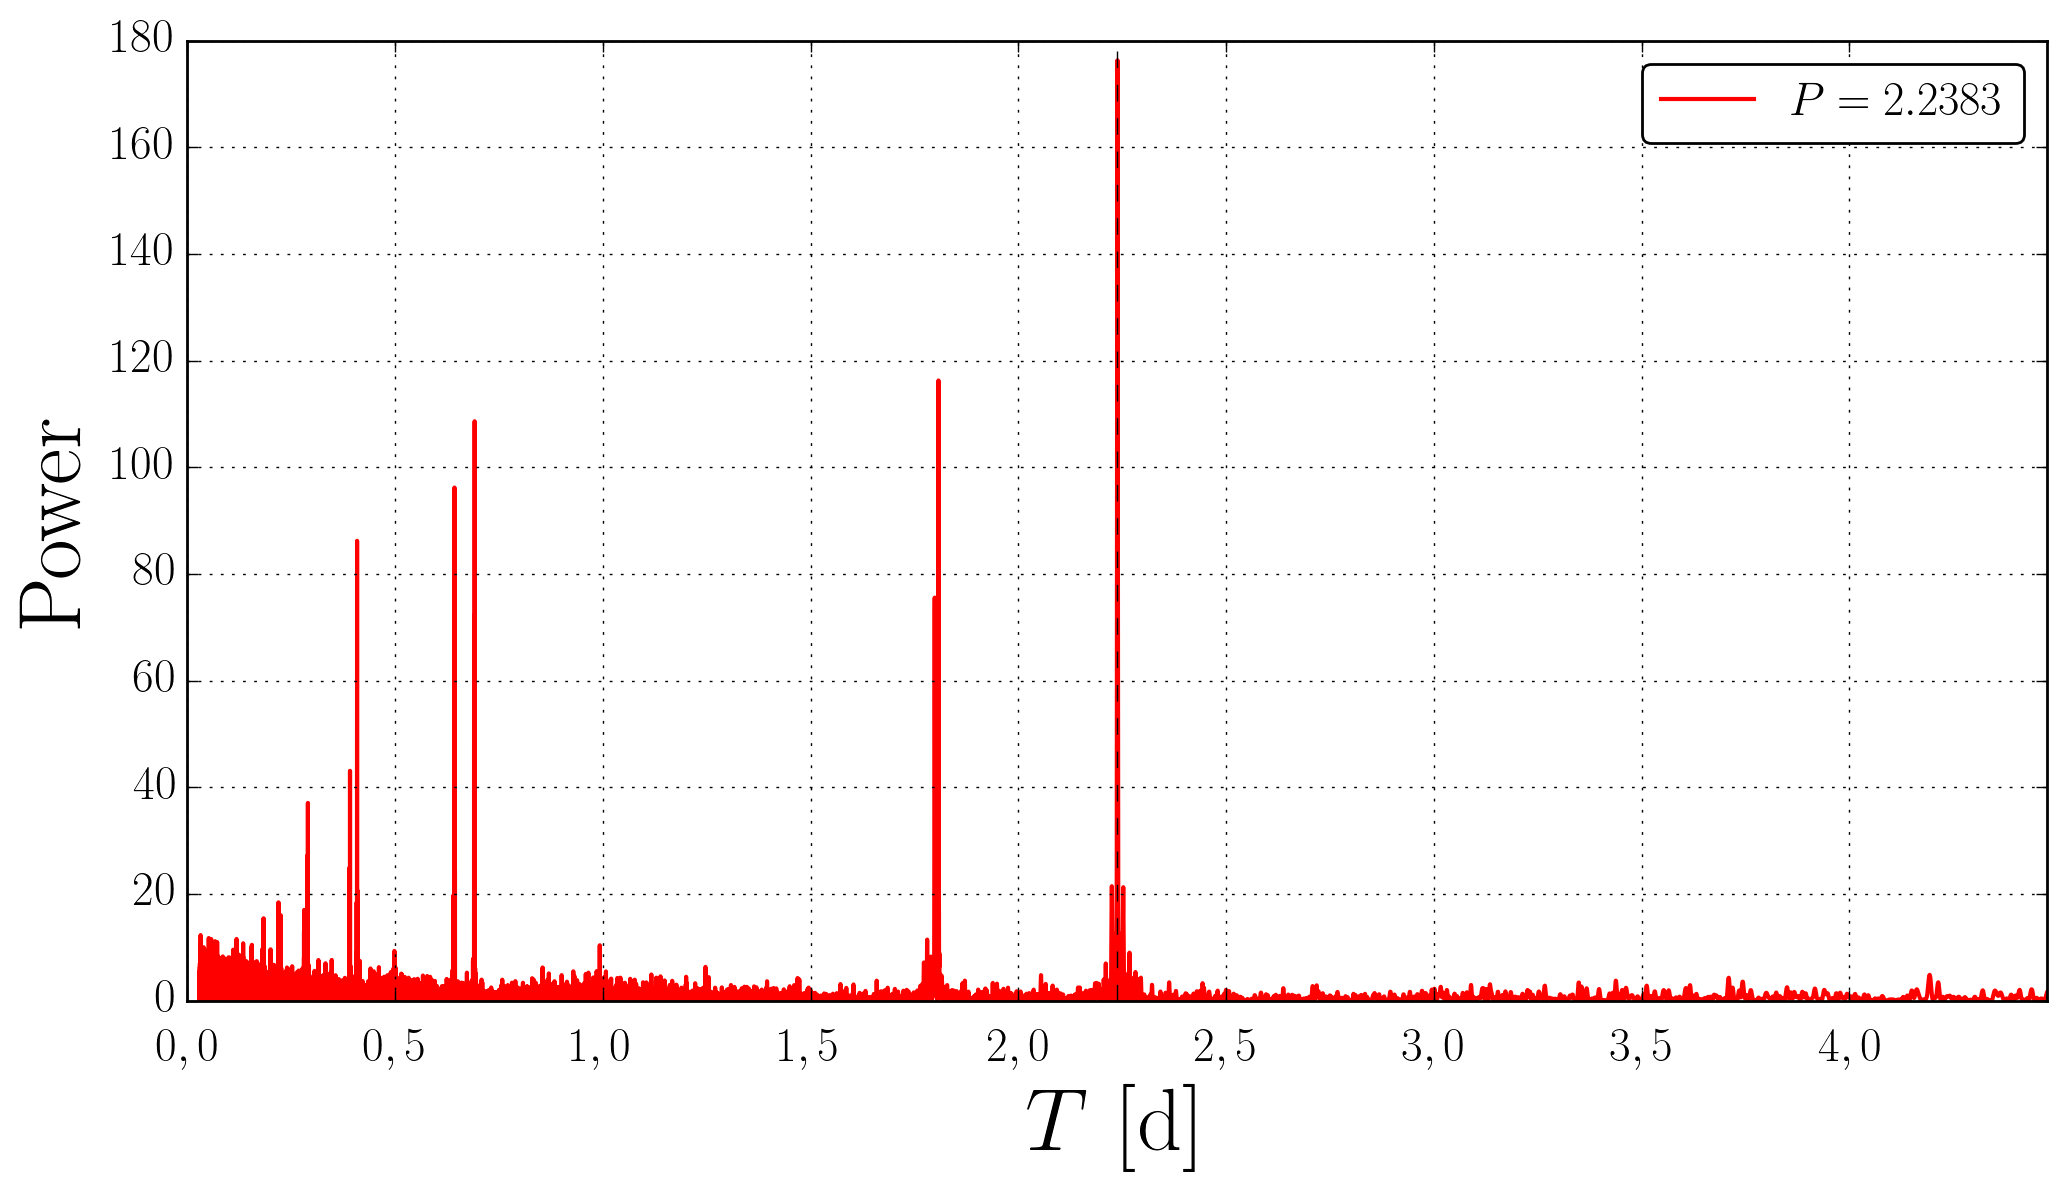
\includegraphics[width=\textwidth]{figures/periodograms/lm0012m20755-fasper.png}
	\end{subfigure}
	\begin{subfigure}[t]{0.49\textwidth}
		\centering
		\label{fig:periodogram-ce}
		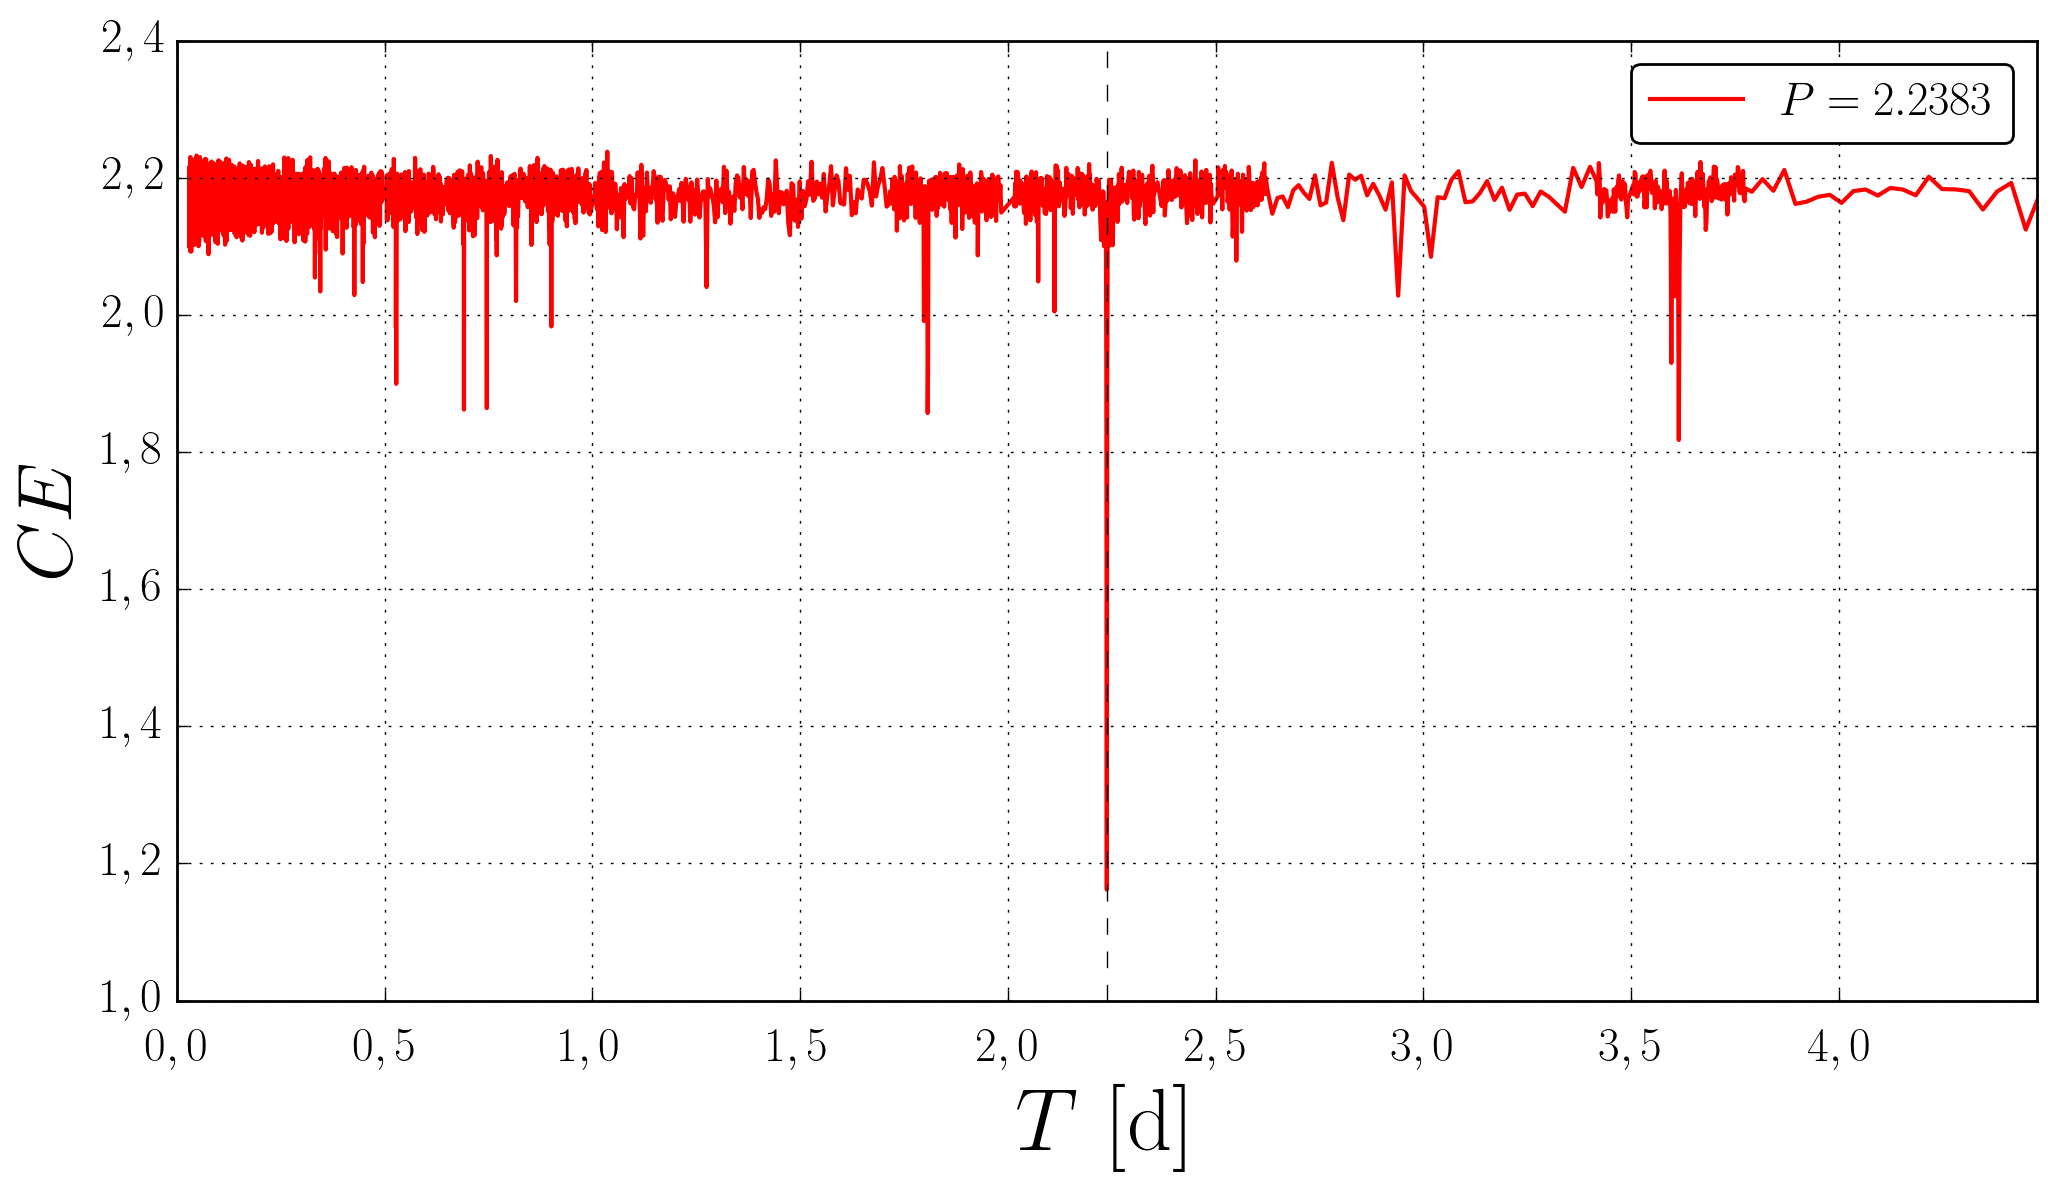
\includegraphics[width=\textwidth]{figures/periodograms/lm0012m20755-ce-adaptive.png}
	\end{subfigure}
	\caption[Lomb--Scargle and CE periodograms for EROS ID \emph{lm0012m20755}]{The left panel shows the Lomb--Scargle periodogram for EROS ID \emph{lm0012m20755}. The extracted period is $T_\text{LS} = 2.2383 \, \unit{d}$. The right panel shows the CE periodogram for the same source, which yields an identical result of $T_\text{CE} = 2.2383 \, \unit{d}$. Both periodograms are centred around the most significant peak.}
	\label{fig:features-periodograms}
\end{figure}

\begin{figure}[h]
	\centering
	\begin{subfigure}[t]{0.49\textwidth}
		\centering
		\label{fig:2e}
		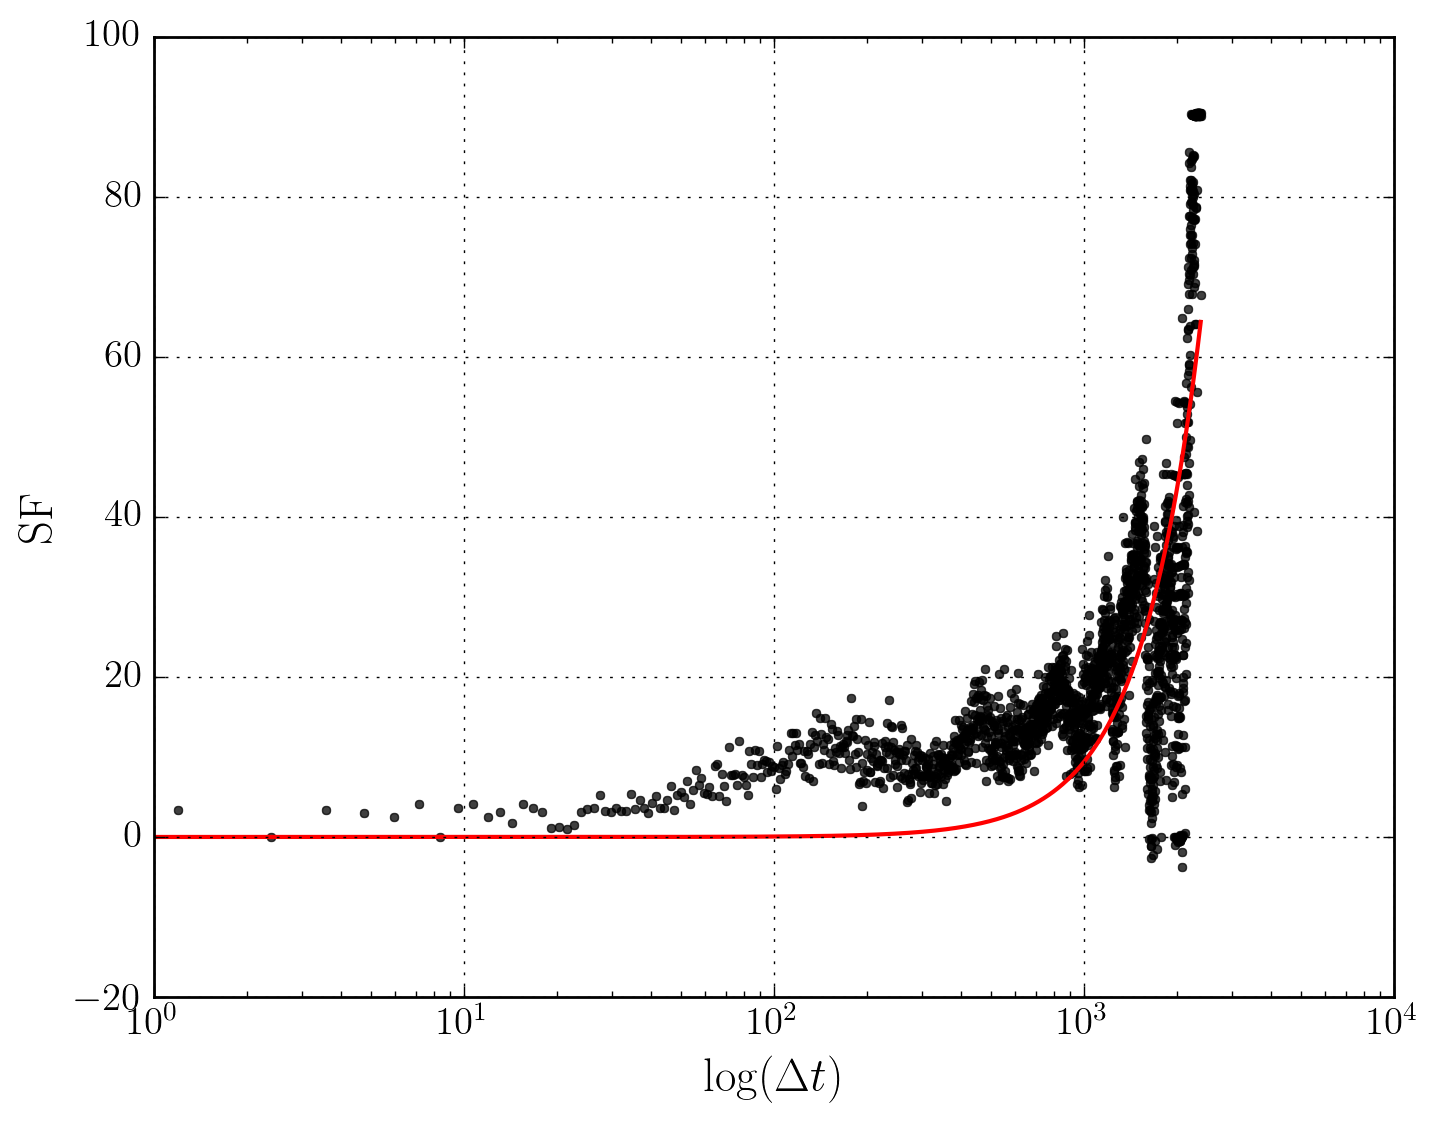
\includegraphics[width=\textwidth]{figures/sf/sf-fit.png}
	\end{subfigure}
	\begin{subfigure}[t]{0.49\textwidth}
		\centering
		\label{fig:2f}
		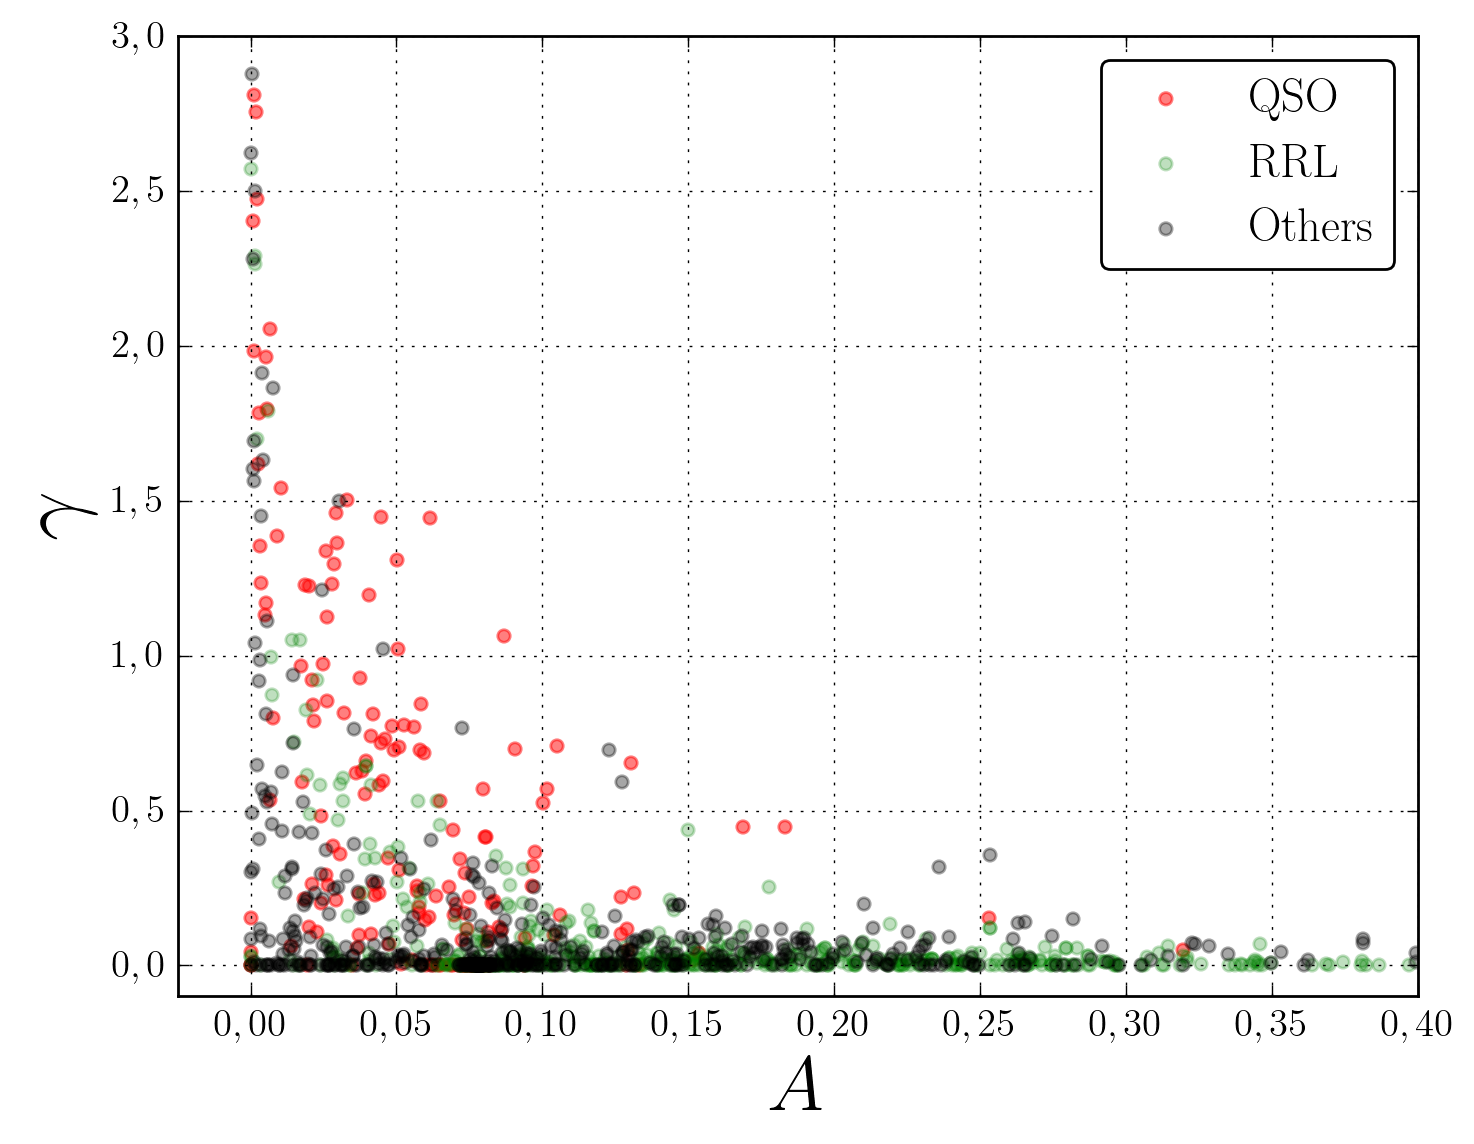
\includegraphics[width=\textwidth]{figures/sf/sf-scatterplot.png}
	\end{subfigure}
	\caption[Visualization of the structure function features]{The left panel shows the structure function fit for a typical quasar in the training set (chosen at random). The right panel shows a scatterplot of 180 randomly sampled \emph{RR Lyrae} and 360 randomly sampled \emph{Others} in addition to the 180 quasars in the data set on the $A$-$\gamma$-plane. We can see that there is indeed some separation, especially in $\gamma$.}
	\label{fig:features-structure-function}
\end{figure}

\begin{figure}[H]
	\centering
	\begin{subfigure}[t]{0.49\textwidth}
		\centering
		\caption{$T_{\text{LS}}$ ($B_E$) vs. $\eta^\phi$ ($B_E$)}
		\label{fig:2a}
		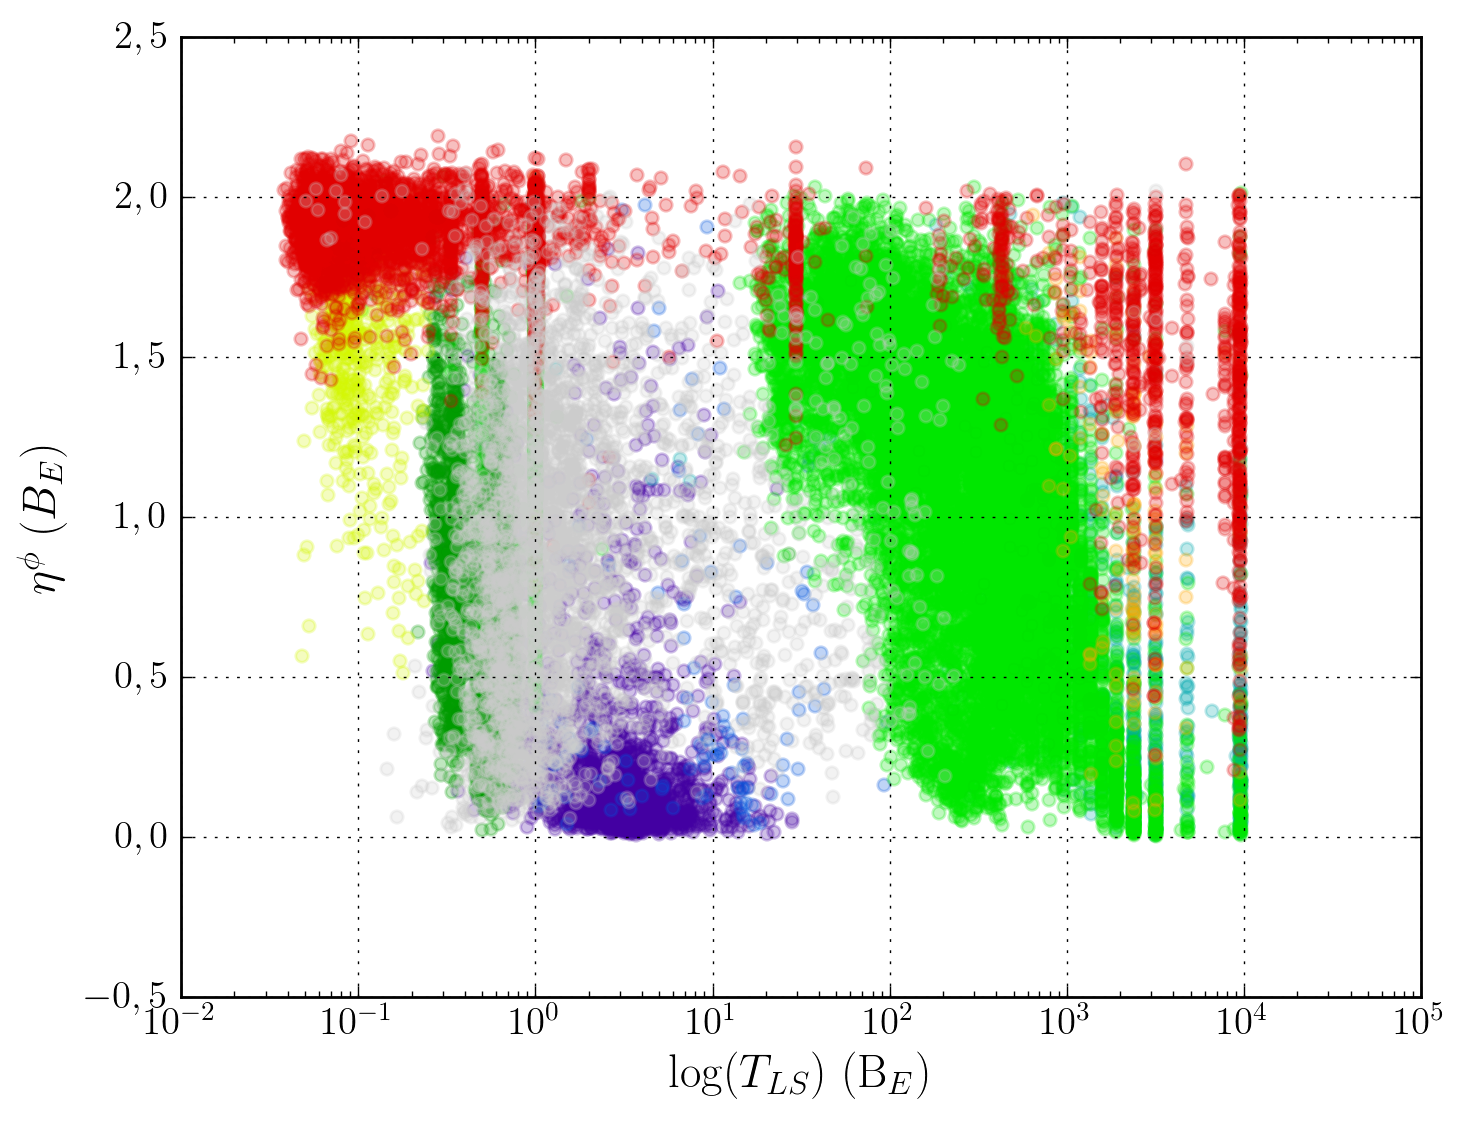
\includegraphics[width=\textwidth]{figures/scatterplots/B-ls-period-B-phase-eta.png}
	\end{subfigure}
	\begin{subfigure}[t]{0.49\textwidth}
		\centering
		\caption{$\eta$ ($B_E$) vs. $\Sigma^\phi$ ($B_E$)}
		\label{fig:2b}
		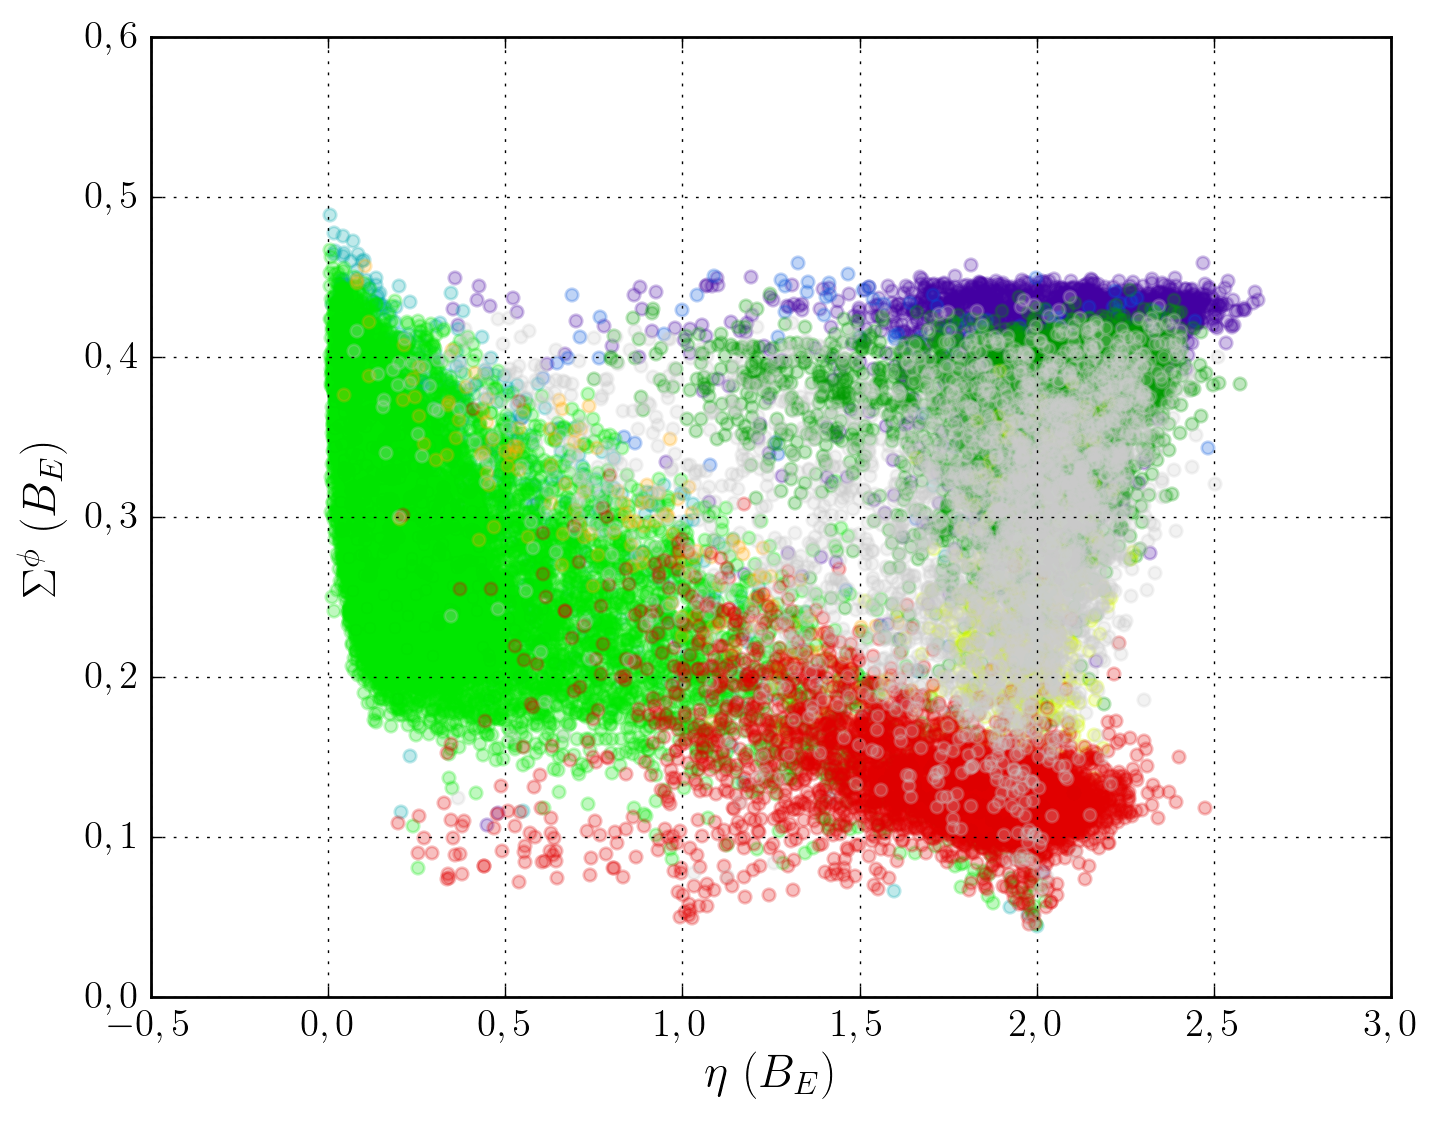
\includegraphics[width=\textwidth]{figures/scatterplots/B-eta-B-phase-cs.png}
	\end{subfigure}
	\begin{subfigure}[t]{0.49\textwidth}
		\centering
		\caption{$\eta$ ($B_E$) vs. $\log(\eta_e)$ ($B_E$)}
		\label{fig:2c}
		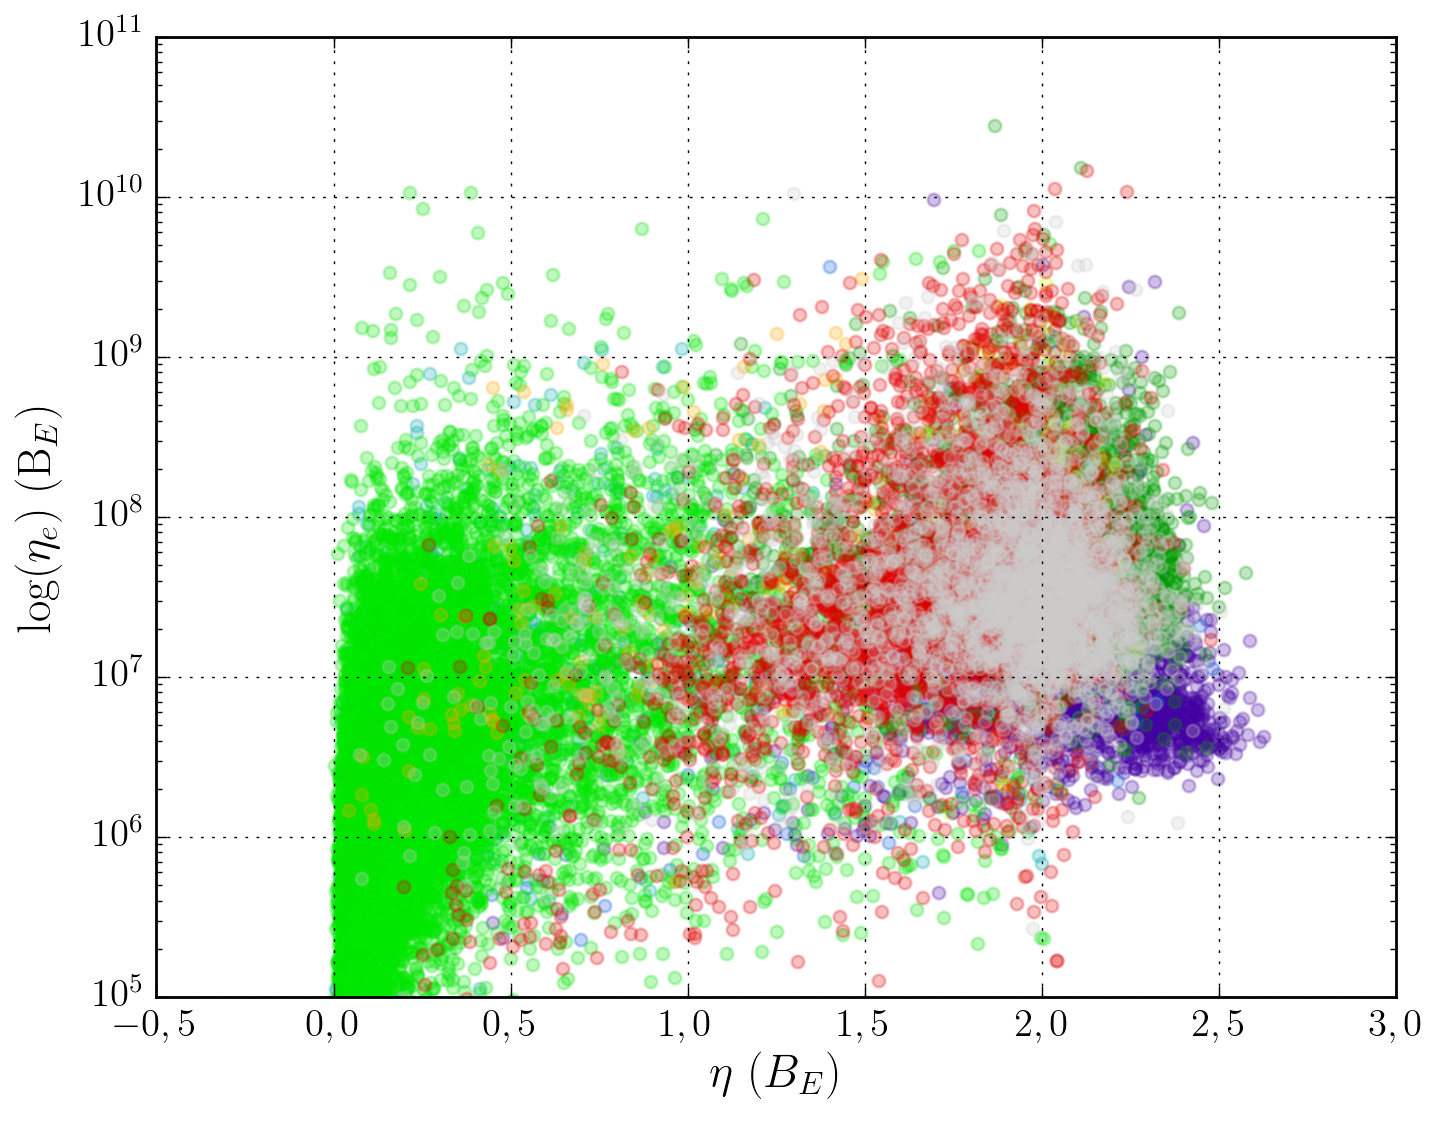
\includegraphics[width=\textwidth]{figures/scatterplots/B-eta-B-eta-e.png}
	\end{subfigure}
	\begin{subfigure}[t]{0.49\textwidth}
		\centering
		\caption{$\mu$ ($B_E$) vs. $\mu$ ($R_E - B_E$)}
		\label{fig:2d}
		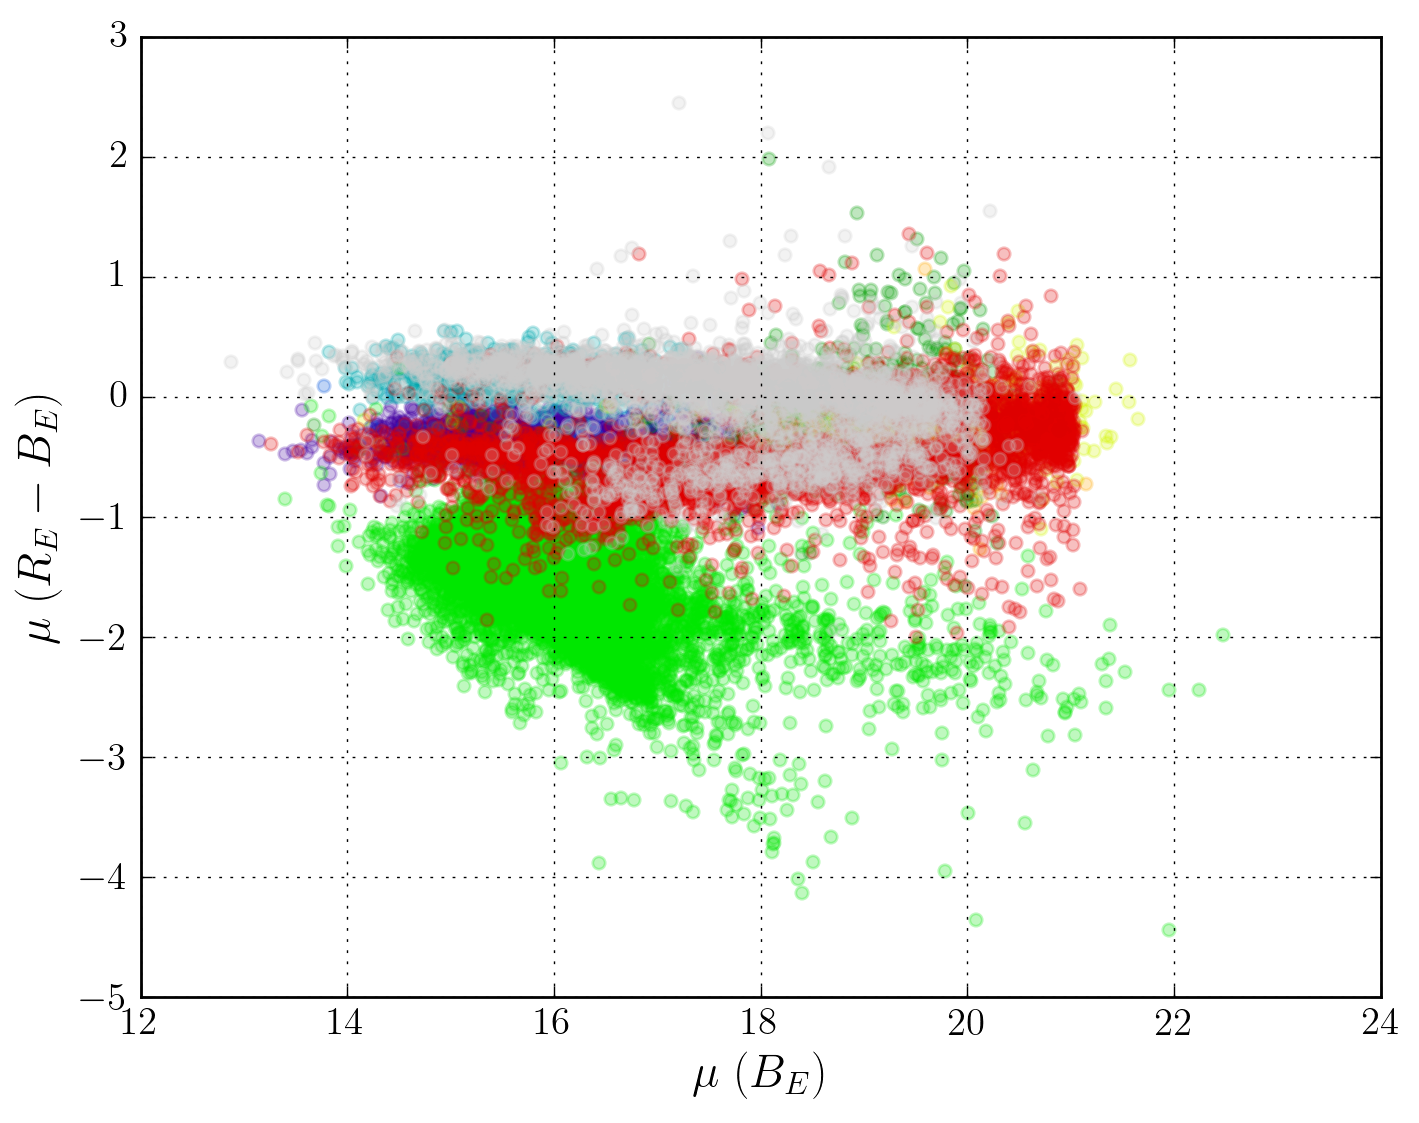
\includegraphics[width=\textwidth]{figures/scatterplots/B-mean-R-B-mean.png}
	\end{subfigure}
	\begin{subfigure}[t]{0.49\textwidth}
		\centering
		\caption{$\Sigma^\phi$ ($B_E$) vs. $\log(\text{IQR})$ ($R_E - B_E$)}
		\label{fig:2e}
		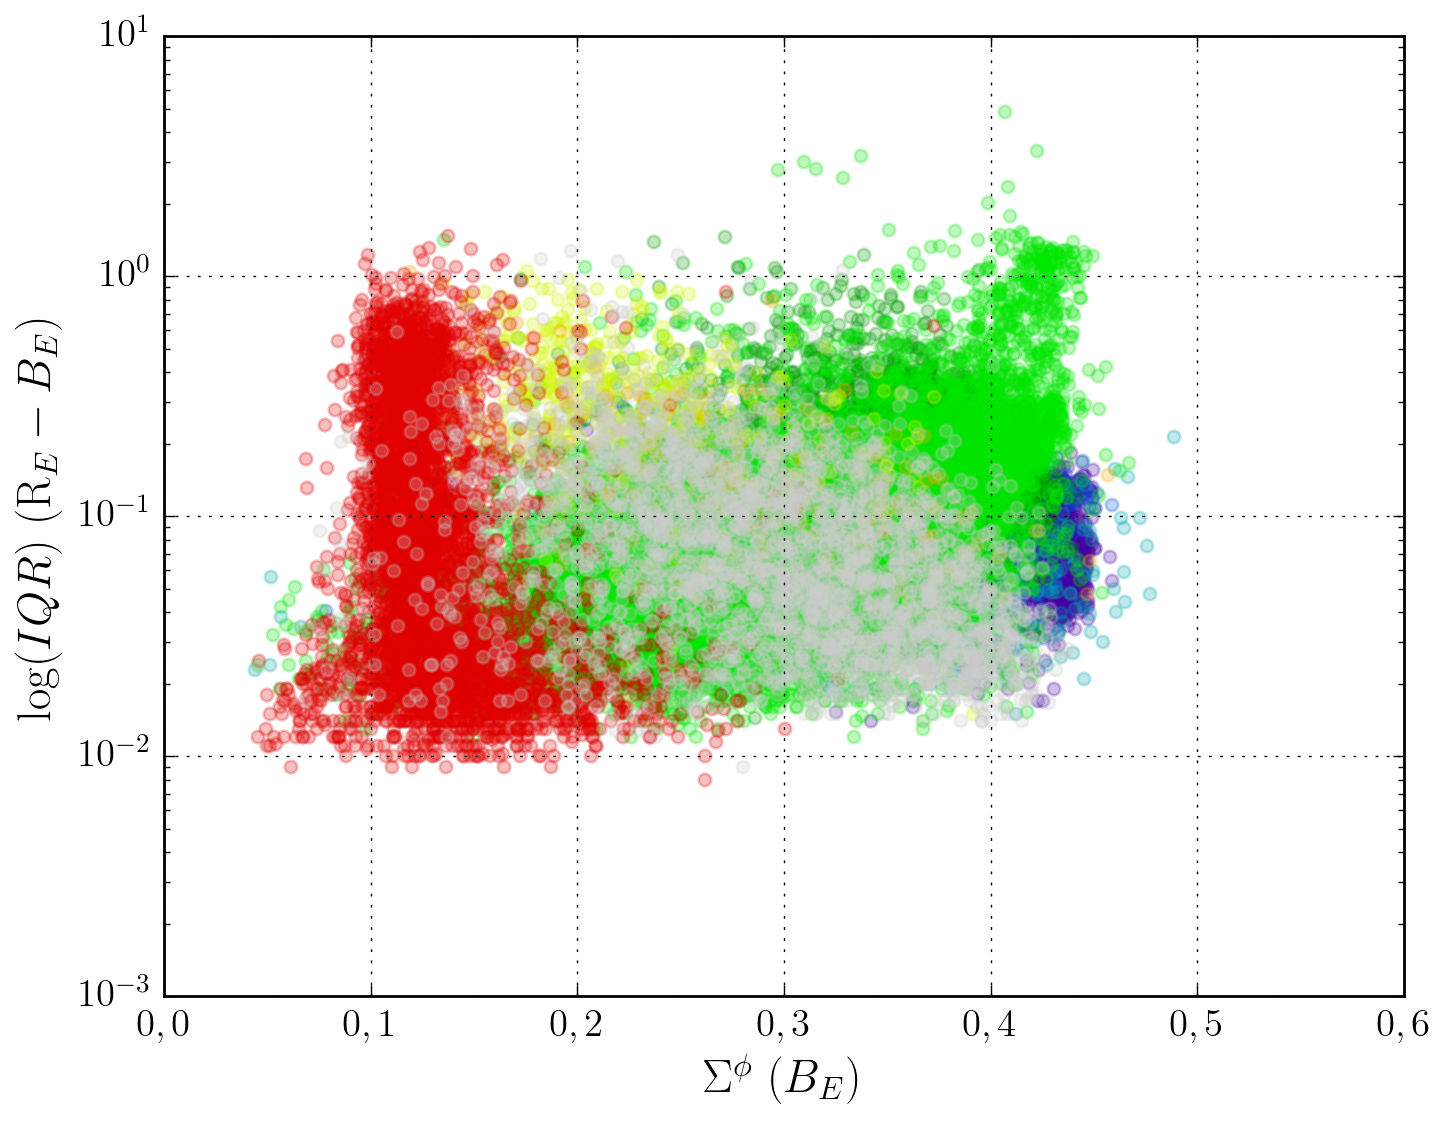
\includegraphics[width=\textwidth]{figures/scatterplots/B-phase-cs-R-B-IQR.png}
	\end{subfigure}
	\begin{subfigure}[t]{0.49\textwidth}
		\centering
		\caption{$\log(T_{\text{LS}})$ ($R_E$) vs. $Q_{25}^\phi$ ($R_E$)}
		\label{fig:2f}
		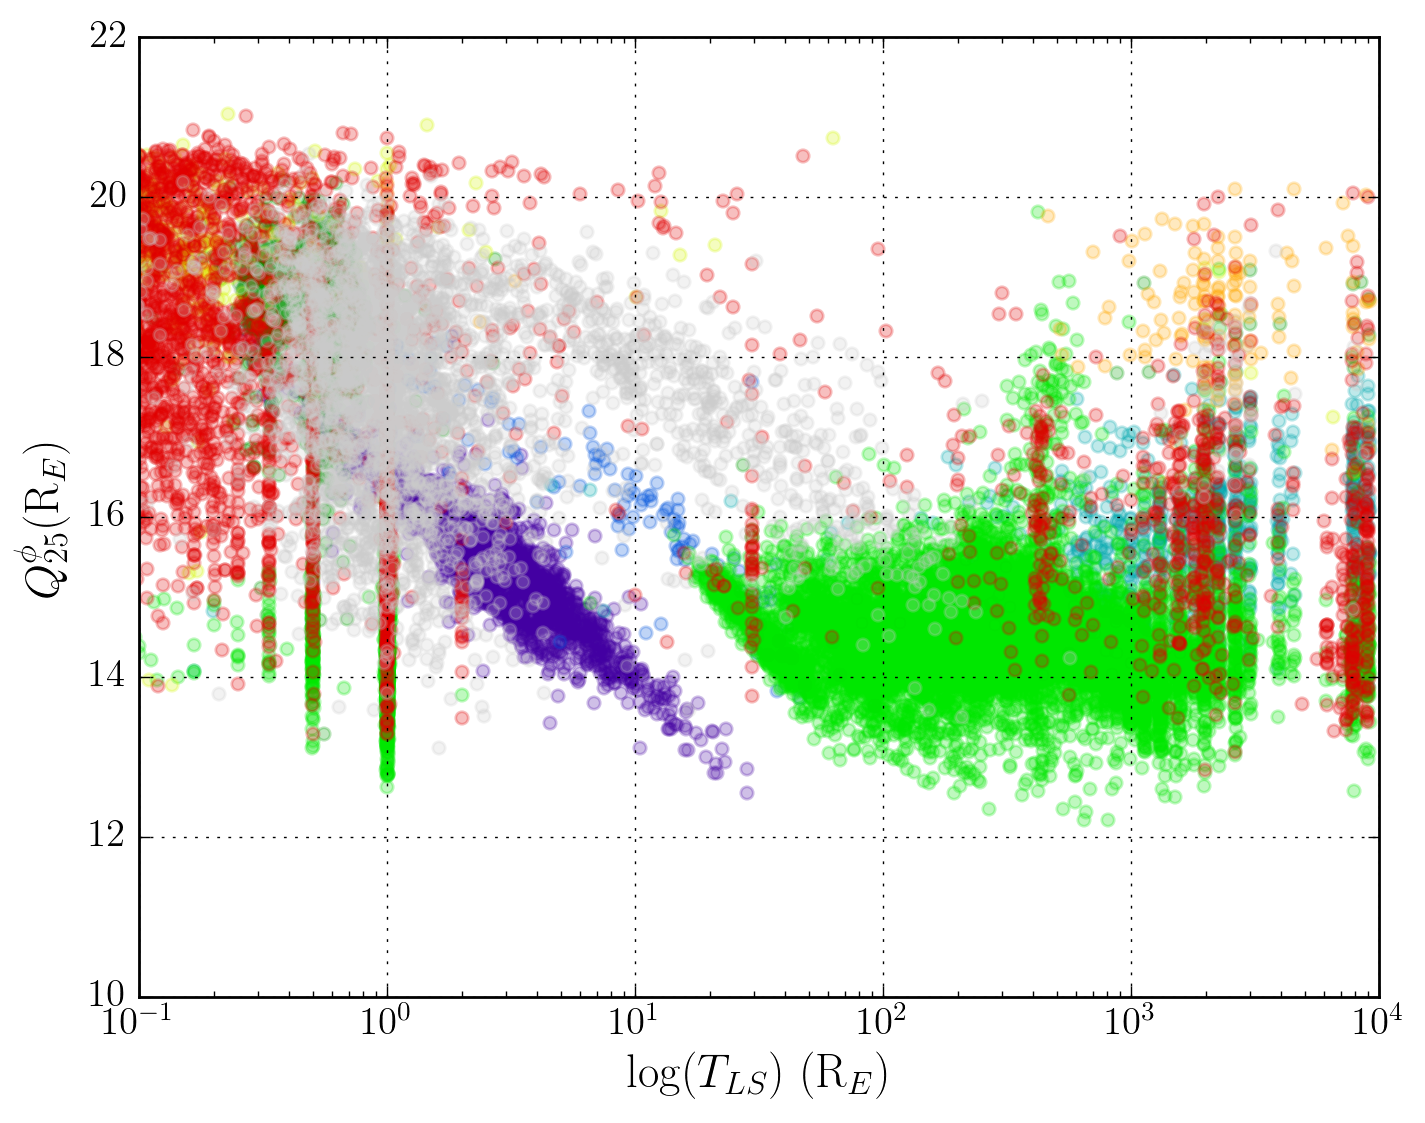
\includegraphics[width=\textwidth]{figures/scatterplots/R-ls-period-R-phase-q25.png}
	\end{subfigure}
	\caption[Scatterplots for different features.]{This figure shows various scatterplots of different features, amongst others $\eta, \eta^\phi$, $\Sigma^\phi$, $T_\text{LS}$, $\text{IQR}$ and $Q_{25}^\phi$, which provide a decent separation in feature space. It is clear to see how the observations form clusters on the respective plane, which are generally contaminated by other sources, since perfect separation is hard to achieve.\\\colorlegend}
	\label{fig:features-scatterplot}
\end{figure}

\section{Performance of the Support Vector Machine}
\label{sec:performance-svm}

The first classifier we try is the Support Vector Machine (SVM) with the RBF kernel $\kernel_{\text{RBF}}$\footnote{We make use of the \emph{scikit--learn} \citep{scikit-learn} Machine Learning library in Python for the implementations of SVM, Random Forest and Gradient Boosted Trees.}. Since SVM is very sensitive to proper feature scaling, we standardize all features by subtracting the mean and dividing by the standard deviation. We optimize the models hyperparameters $C$ and $\gamma$ for the average, weighted $F_1$-score by performing a $5$-fold cross--validation on subsequently finer grids. The results of this procedure are visualized in figure \ref{fig:gridsearch-svm-superclasses}, beginning with a coarse grid on the upper left corner, narrowing down the optimum on a finer grids (left to right, top to bottom) towards a global optimum (lower right). The optimal hyperparameters we find for the superclass classification are $C = 4.67 \cdot 10^{2}$ and $\gamma = 1.69 \cdot 10^{-3}$. The confusion matrix is shown in table \ref{tab:svm-confusion-matrix-superclasses}, where the columns show the predicted labels, while the rows show the true label. Consequently, the diagonal shows \emph{true positives}. All confusion matrices in this report were generated by combining the $k$ confusion matrices of each individual model during $k$-fold cross--validation. The average, weighted $F_1$-score is $(97.25 \, \pm \, 0.25) \, \%$\footnote{The error estimate can be interpreted as \emph{generalization error}. More on this in the discussion (section \ref{sec:discussion}).}.\\

\begin{table}[h]
\centering
\resizebox{\textwidth}{!}{
\begin{tabular}{c|ccccccccc|c}
\toprule
                   & BV        & CEPH       & DSCT      & EB         & LPV         & NonVar     & QSO       & RRL        & T2CEPH   & $\Sigma $ \\
\midrule
BV                 & {\bfseries 762} &            &           &     12     &     1       &     19     &      1    &            &     1    &     796   \\
CEPH               &     2     & {\bfseries 2218} &           &     13     &     5       &     3      &           &     28     &    12    &    2281   \\
DSCT               &           &      5     & {\bfseries 453} &     8      &             &     17     &           &     28     &          &     511   \\
EB                 &    16     &      16    &     10    & {\bfseries 3336} &     50      &     54     &      5    &     46     &     5    &    3538   \\
LPV                &     5     &      5     &           &     46     & {\bfseries 15884} &     51     &      2    &     2      &          &   15995   \\
NonVar             &    15     &      1     &     14    &     48     &     65      & {\bfseries 4621} &      24   &     3      &          &    4791   \\
QSO                &     2     &      1     &           &     1      &      1      &     30     & {\bfseries 144} &     1      &          &     180   \\
RRL                &           &      27    &     34    &     60     &      4      &     7      &           & {\bfseries 4336} &     2    &    4470   \\
T2CEPH             &     1     &      23    &           &     16     &      6      &     1      &           &     11     & {\bfseries 63} &     121   \\
\bottomrule
Recall ($\%$)      &   95.73   &     97.24  &   88.65   &    94.29   &    99.31    &   96.45    &    80.00  &    97.00   &   52.07  &           \\
\hline
Precision ($\%$)   &   94.89   &     96.60  &   88.65   &    94.24   &    99.18    &   96.21    &    81.82  &    97.33   &   75.90  &           \\
\hline
$F_1$ score ($\%$) &   95.31   &     96.92  &   88.65   &    94.26   &    99.24    &   96.33    &    80.90  &    97.16   &   61.77  & 97.25 $\pm$ 0.25 \\
\bottomrule

\end{tabular}
}
\caption{This table shows the confusion matrix for the SVM superclass classification on the EROS--2 data set with $C = 4.67 \cdot 10^{2}$ and $\gamma = 1.69 \cdot 10^{-3}$. The columns show the predicted labels, while the rows show the true label.}
\label{tab:svm-confusion-matrix-superclasses}
\end{table}

\begin{figure}[ht!]
	\centering
	\begin{subfigure}[t]{0.49\textwidth}
		\centering
		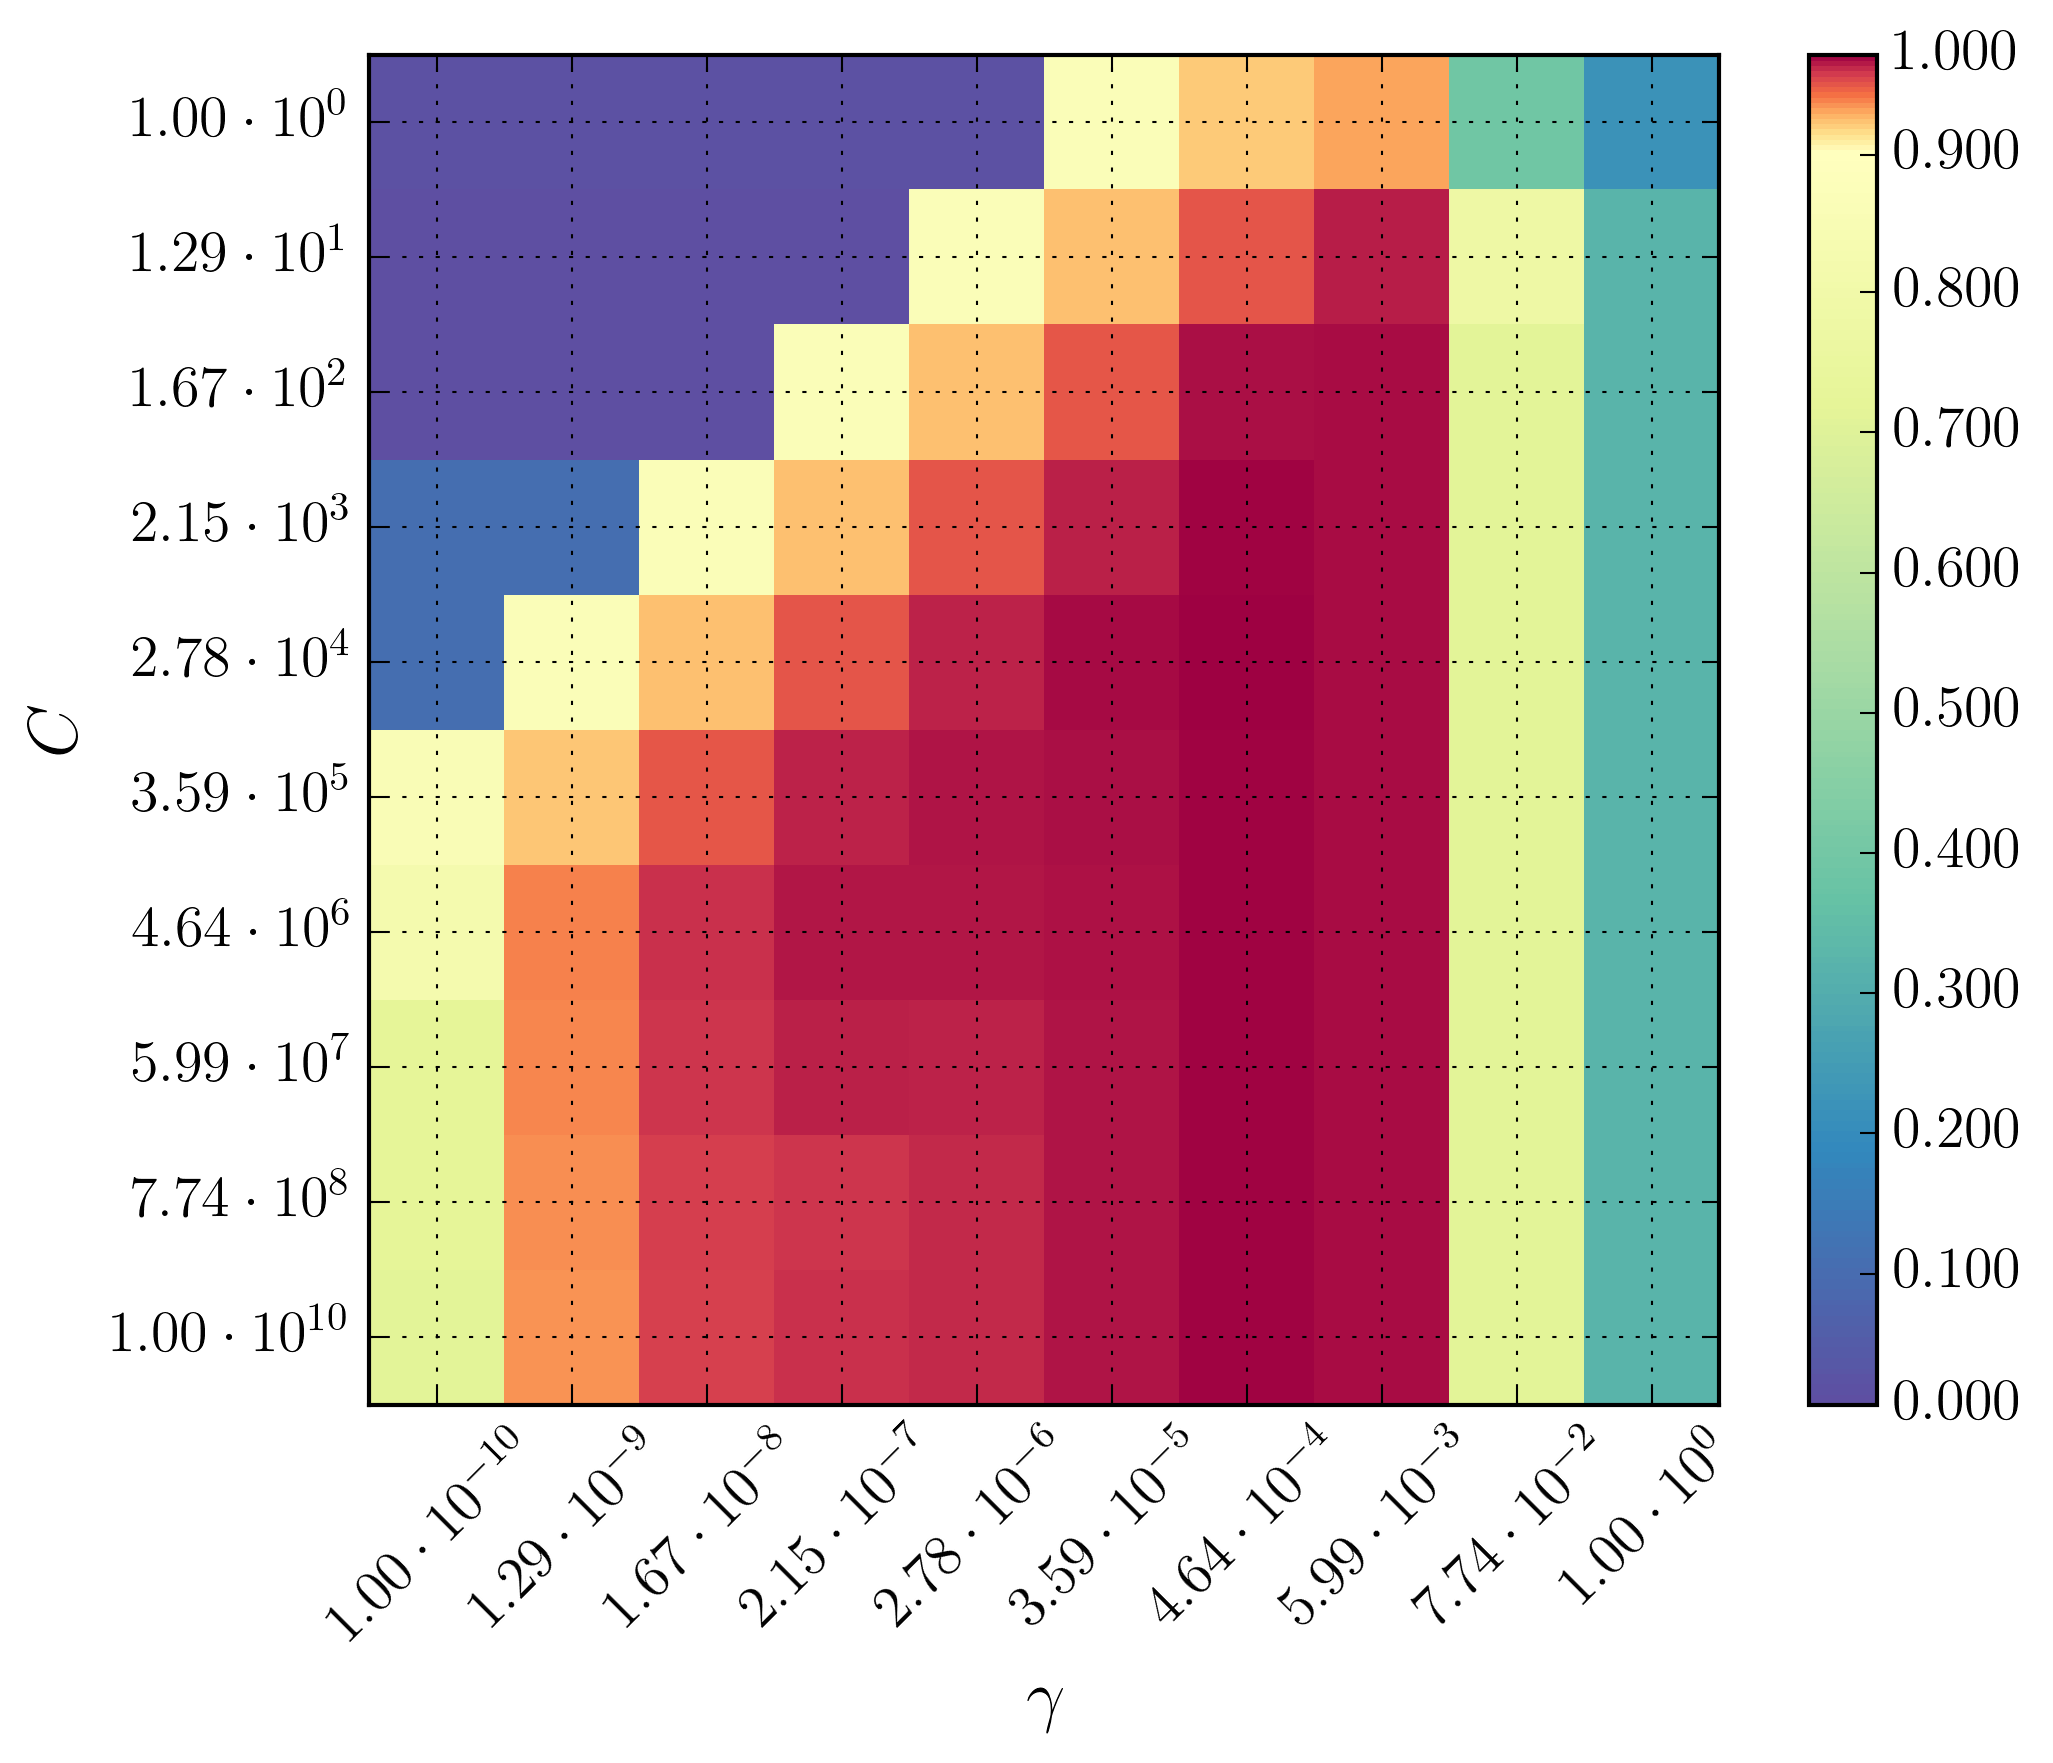
\includegraphics[width=\textwidth]{figures/gridsearch/svm/superclasses/svm-superclasses-01.png}
	\end{subfigure}
	\begin{subfigure}[t]{0.49\textwidth}
		\centering
		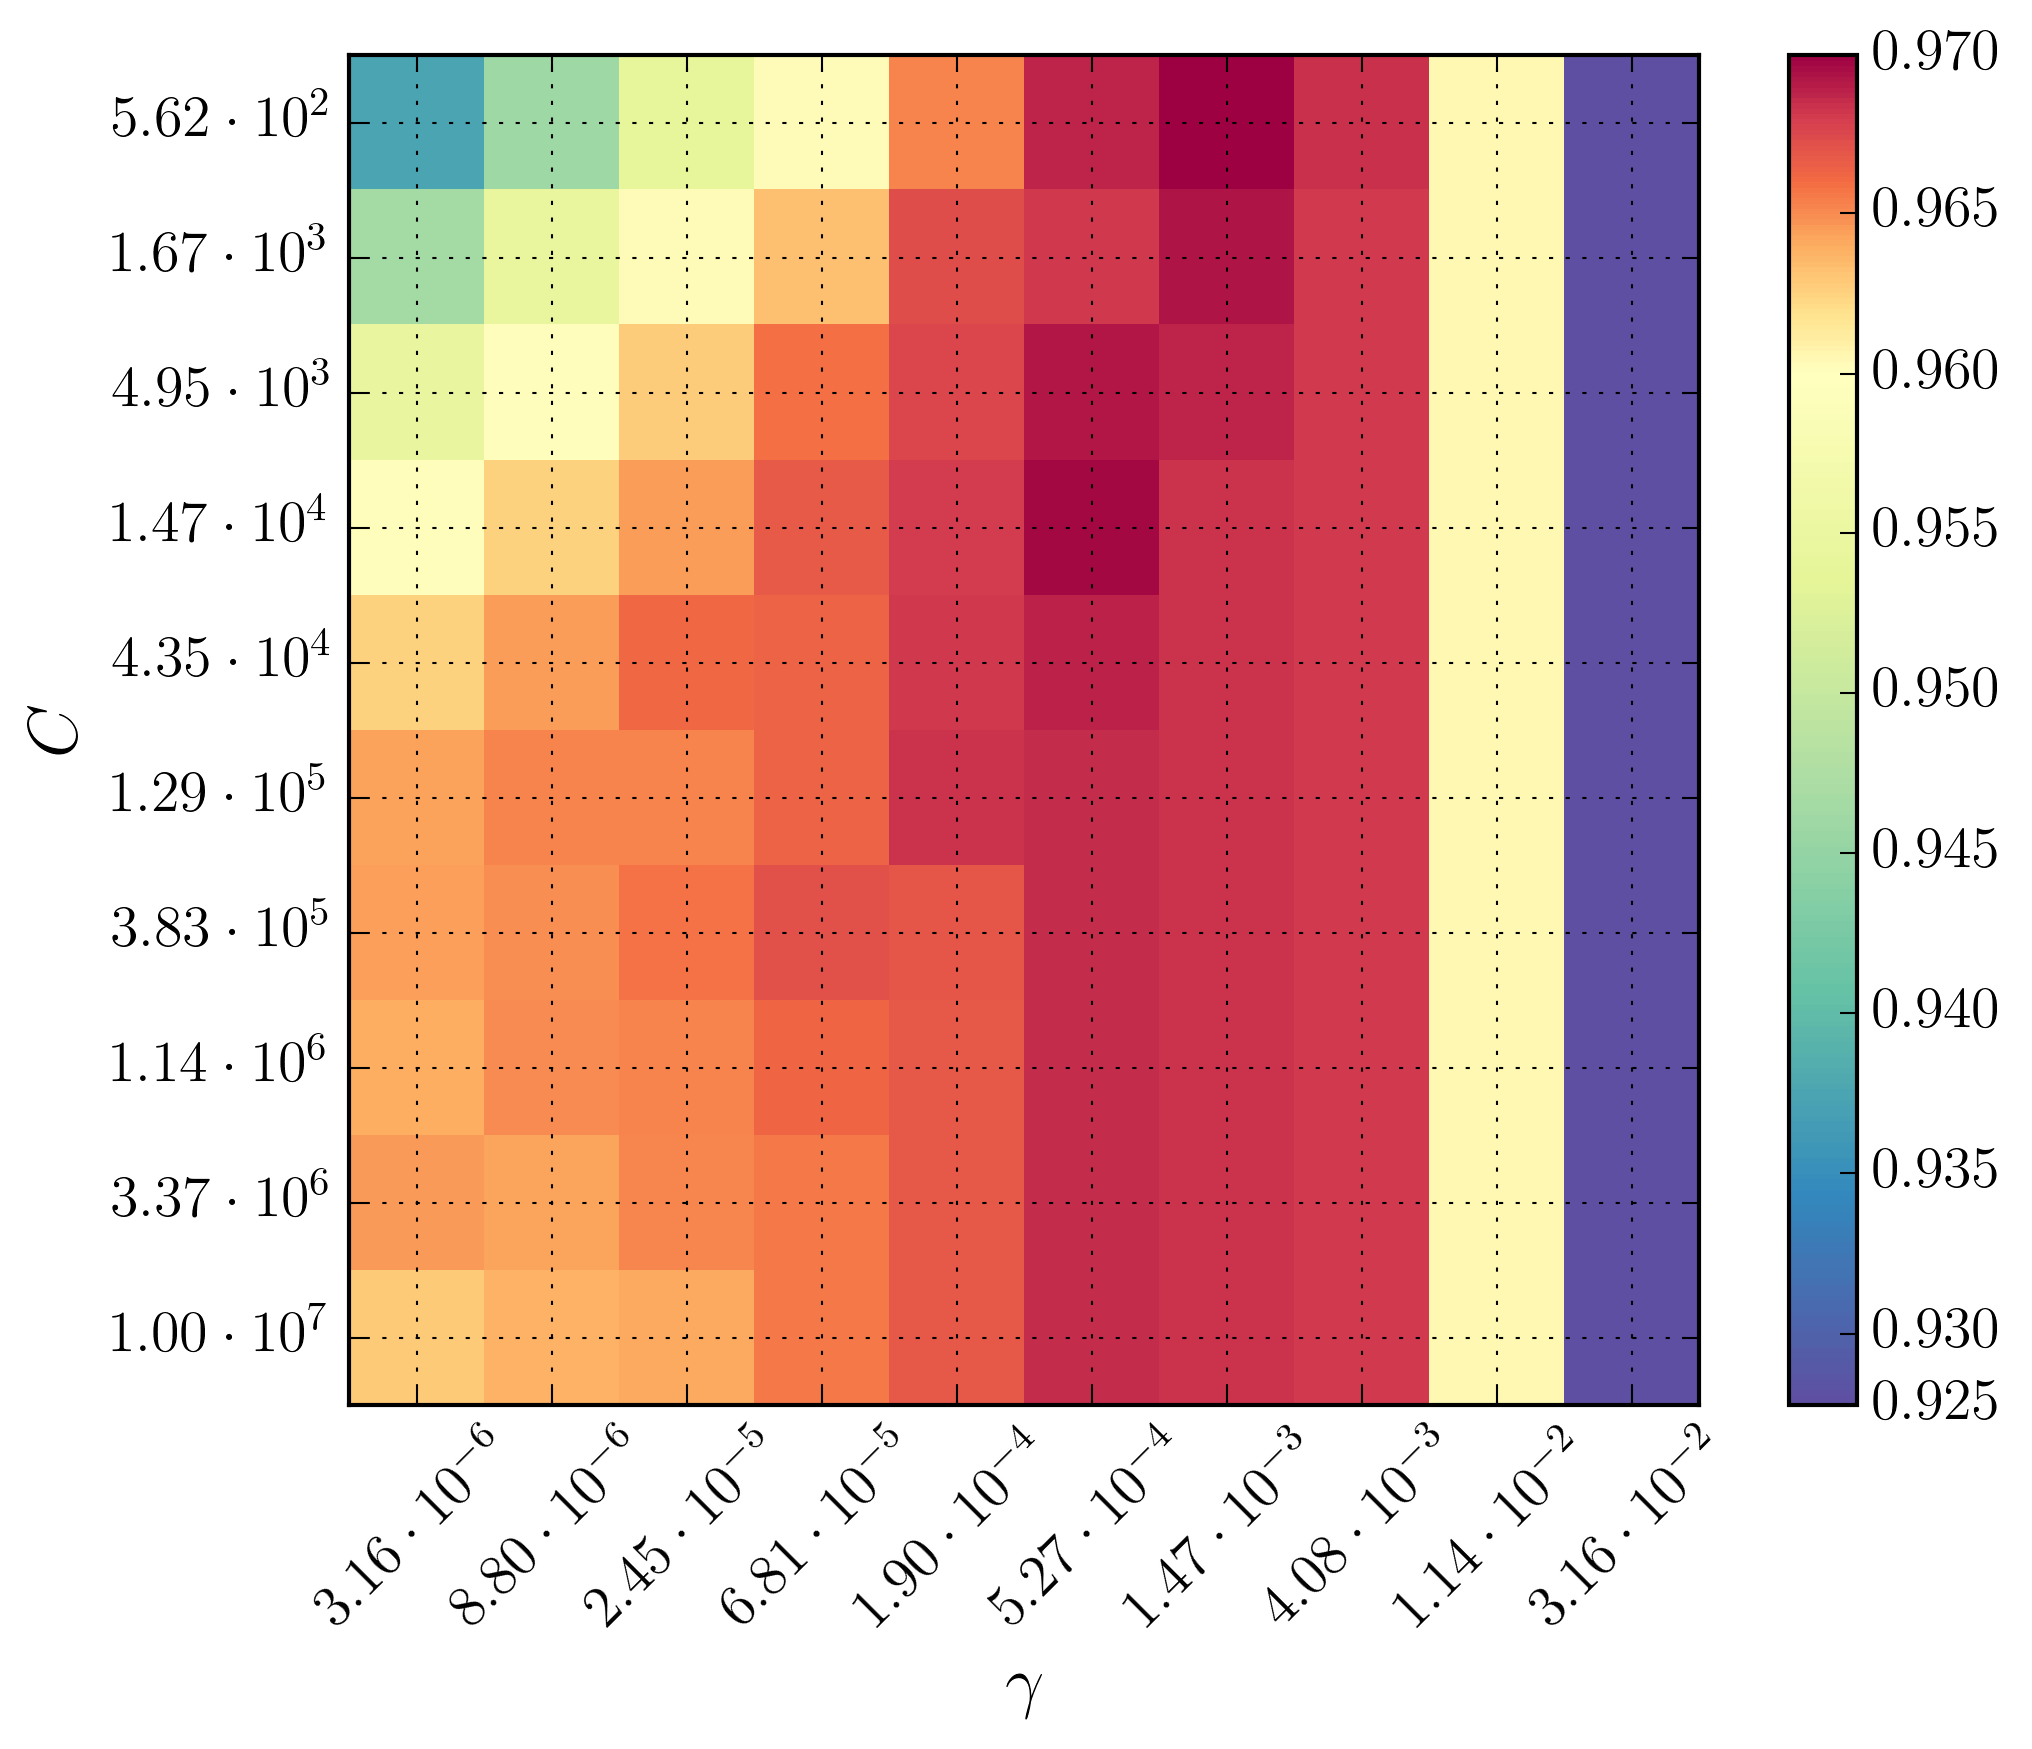
\includegraphics[width=\textwidth]{figures/gridsearch/svm/superclasses/svm-superclasses-02.png}
	\end{subfigure}
	\begin{subfigure}[t]{0.49\textwidth}
		\centering
		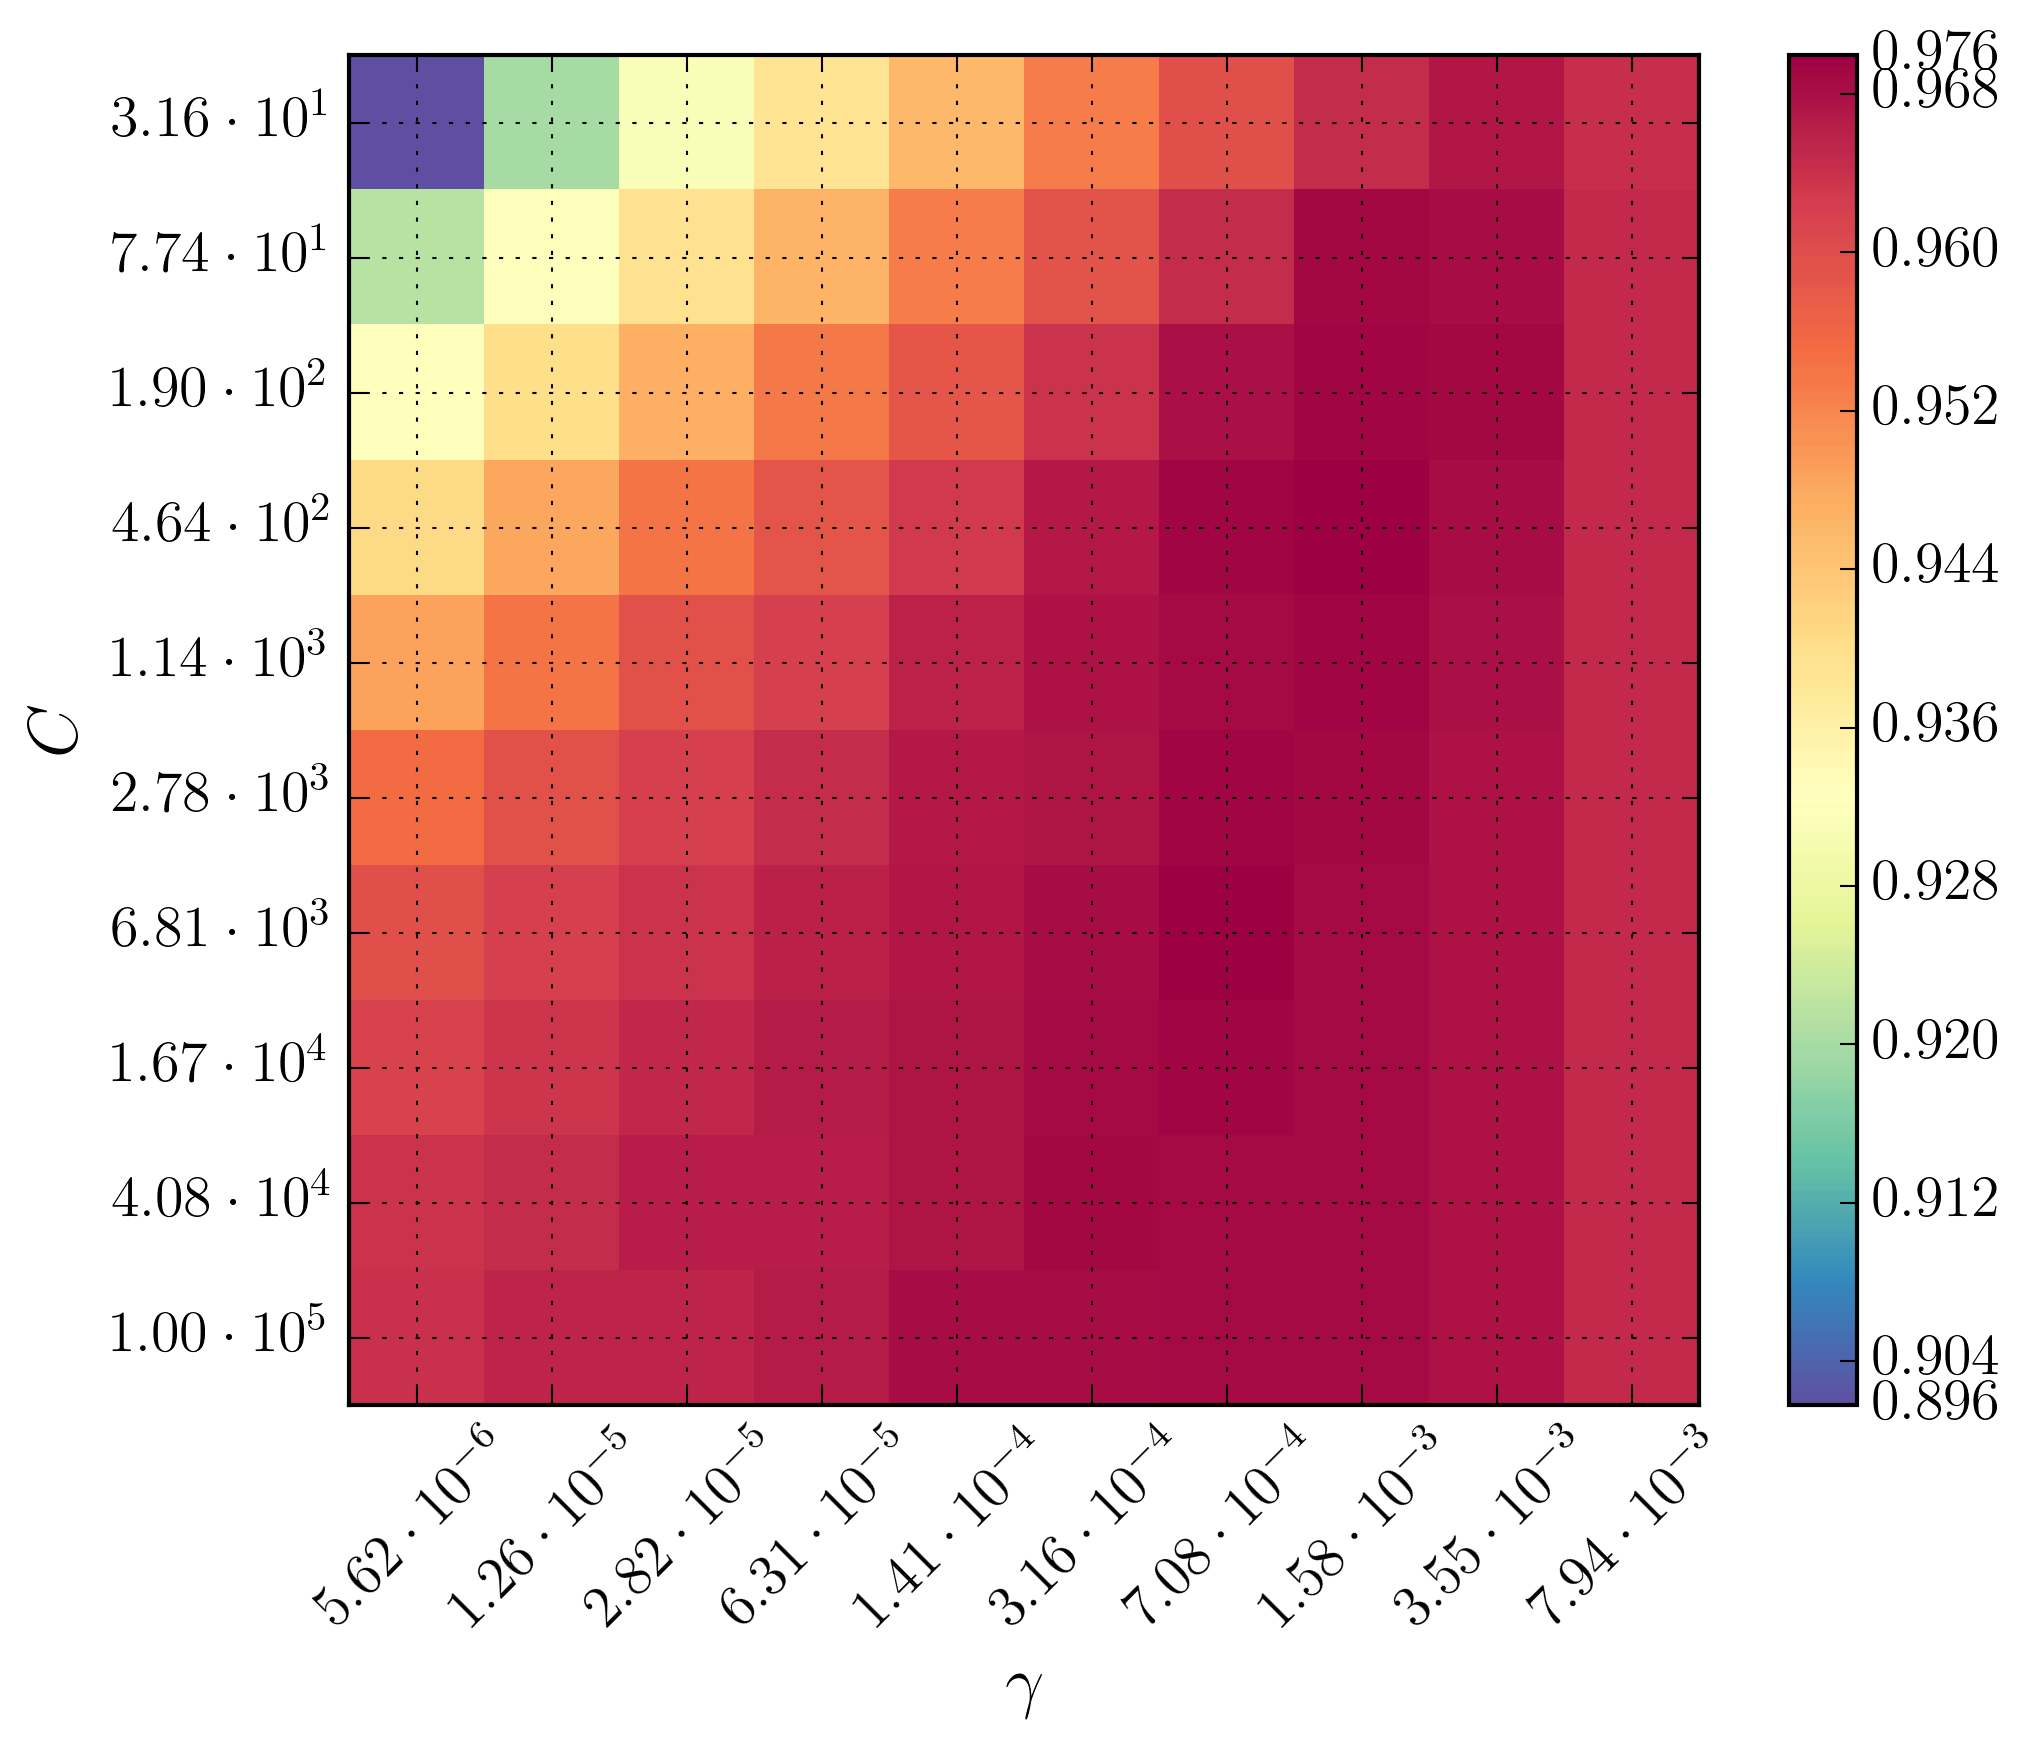
\includegraphics[width=\textwidth]{figures/gridsearch/svm/superclasses/svm-superclasses-03.png}
	\end{subfigure}
	\begin{subfigure}[t]{0.49\textwidth}
		\centering
		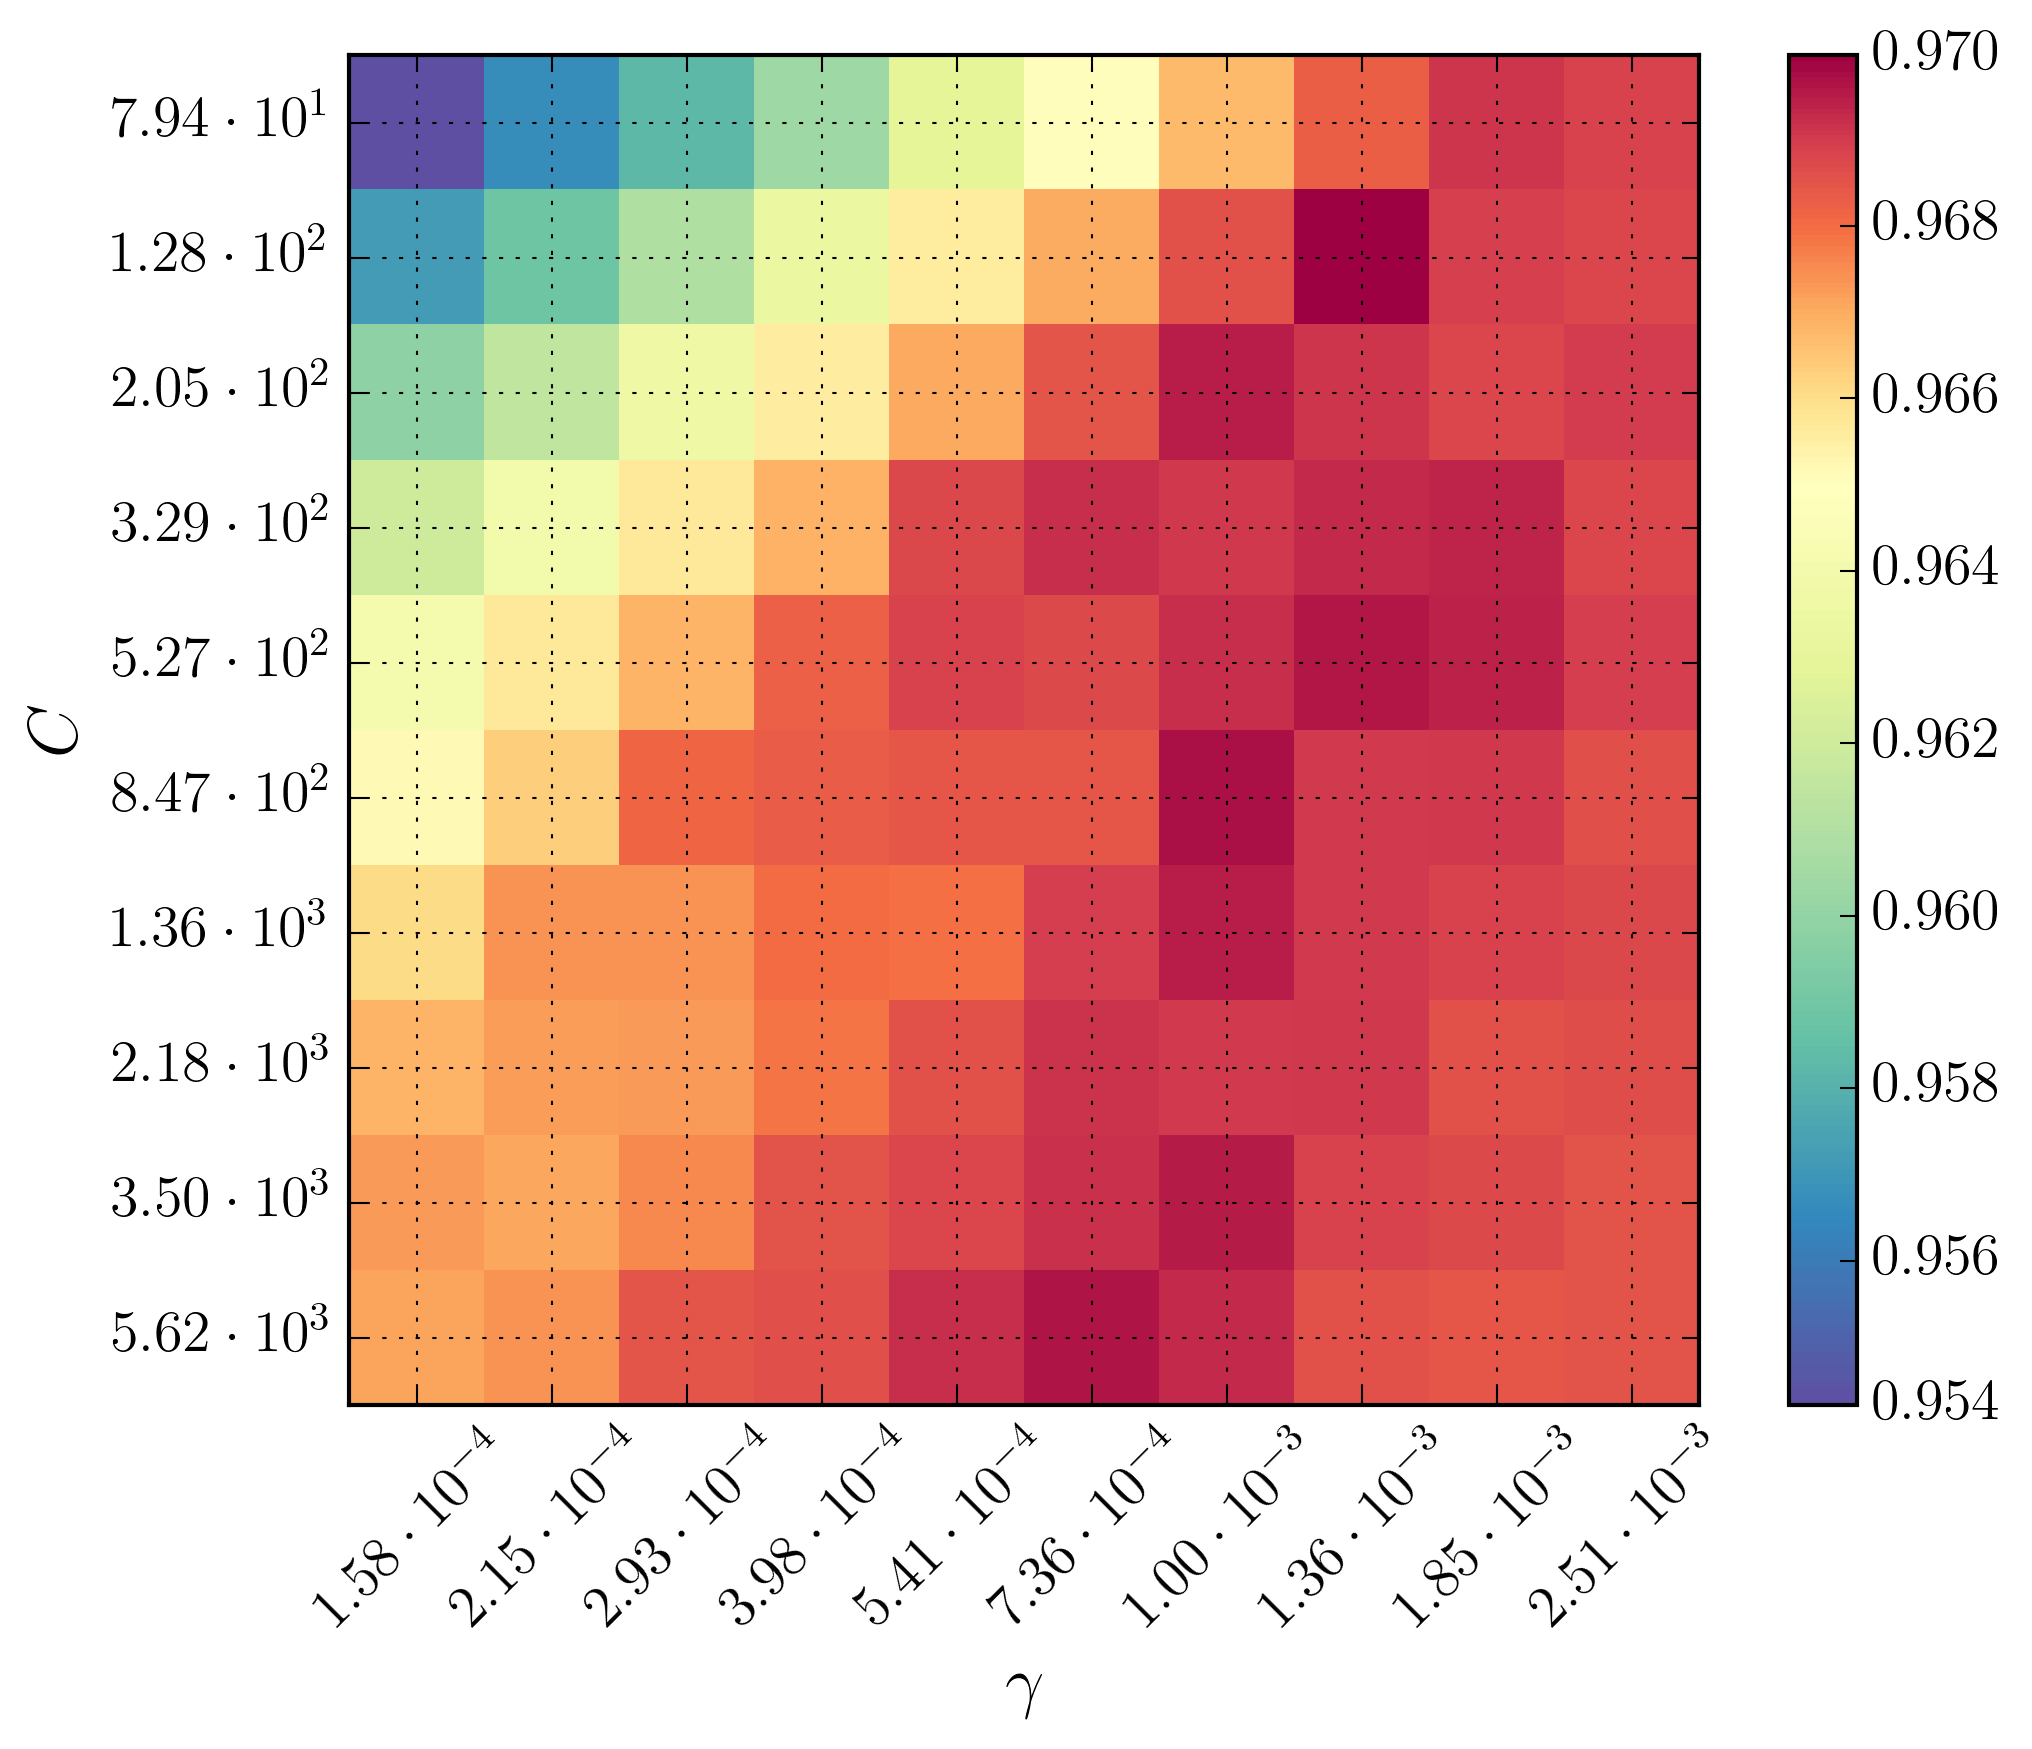
\includegraphics[width=\textwidth]{figures/gridsearch/svm/superclasses/svm-superclasses-04.png}
	\end{subfigure}
	\begin{subfigure}[t]{0.49\textwidth}
		\centering
		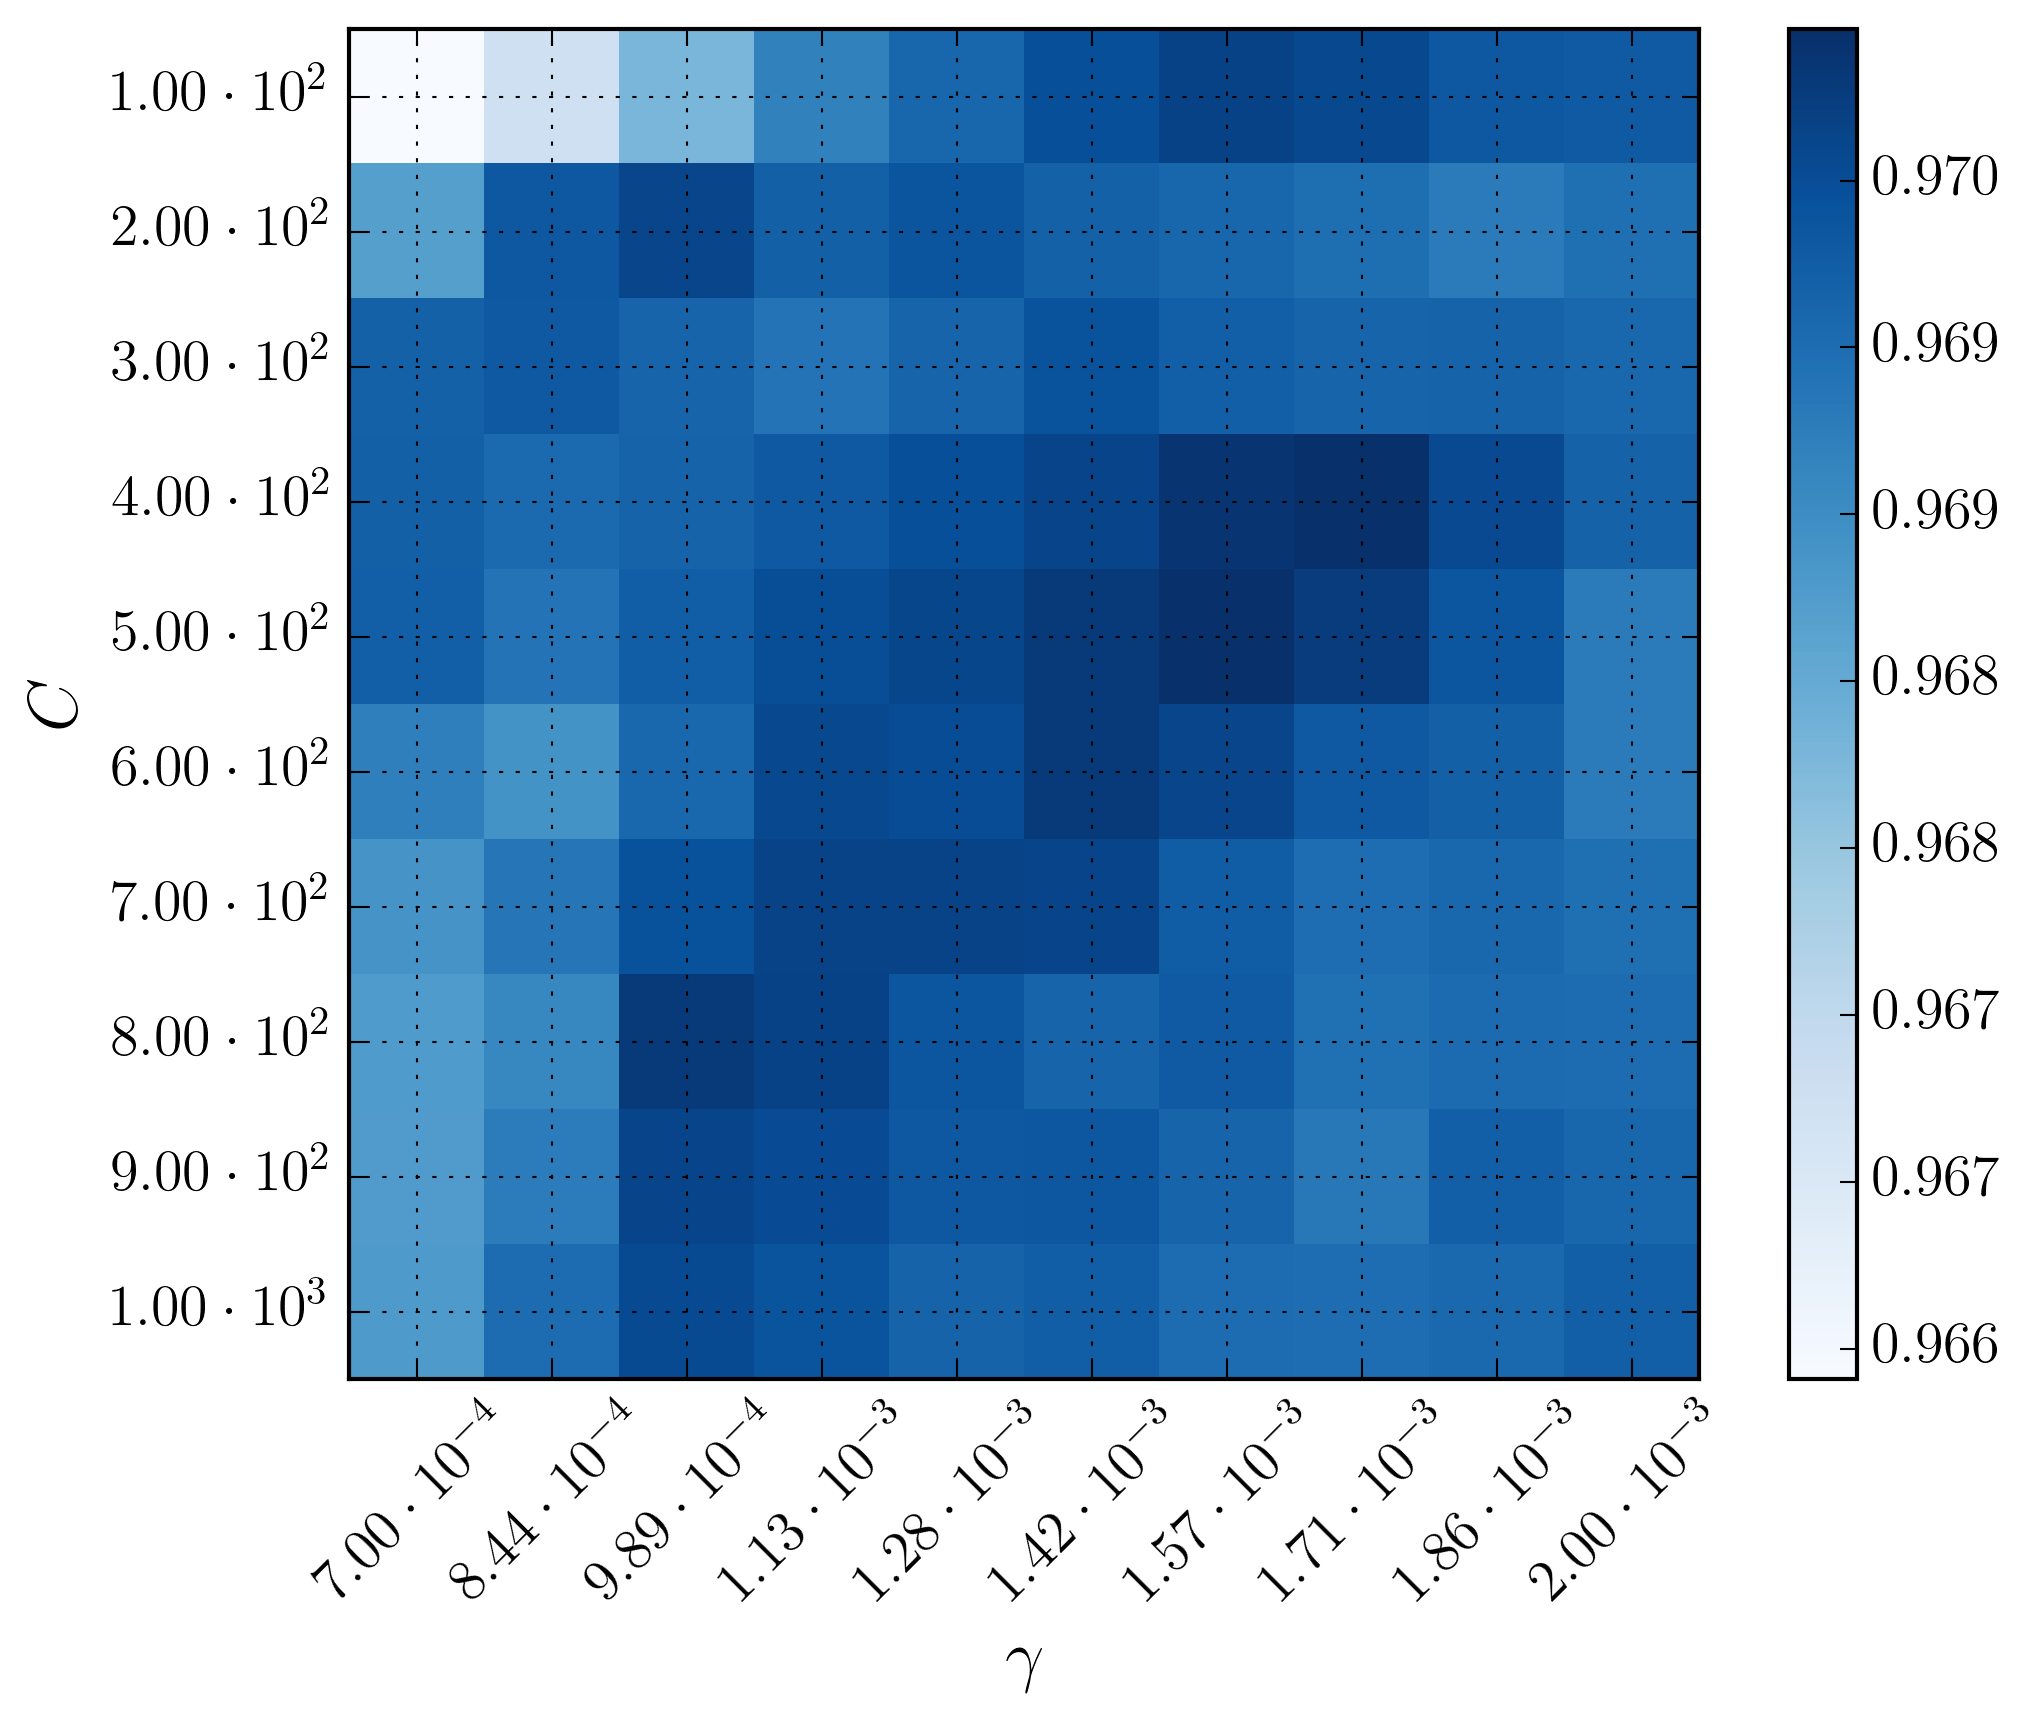
\includegraphics[width=\textwidth]{figures/gridsearch/svm/superclasses/svm-superclasses-05.png}
	\end{subfigure}
	\begin{subfigure}[t]{0.49\textwidth}
		\centering
		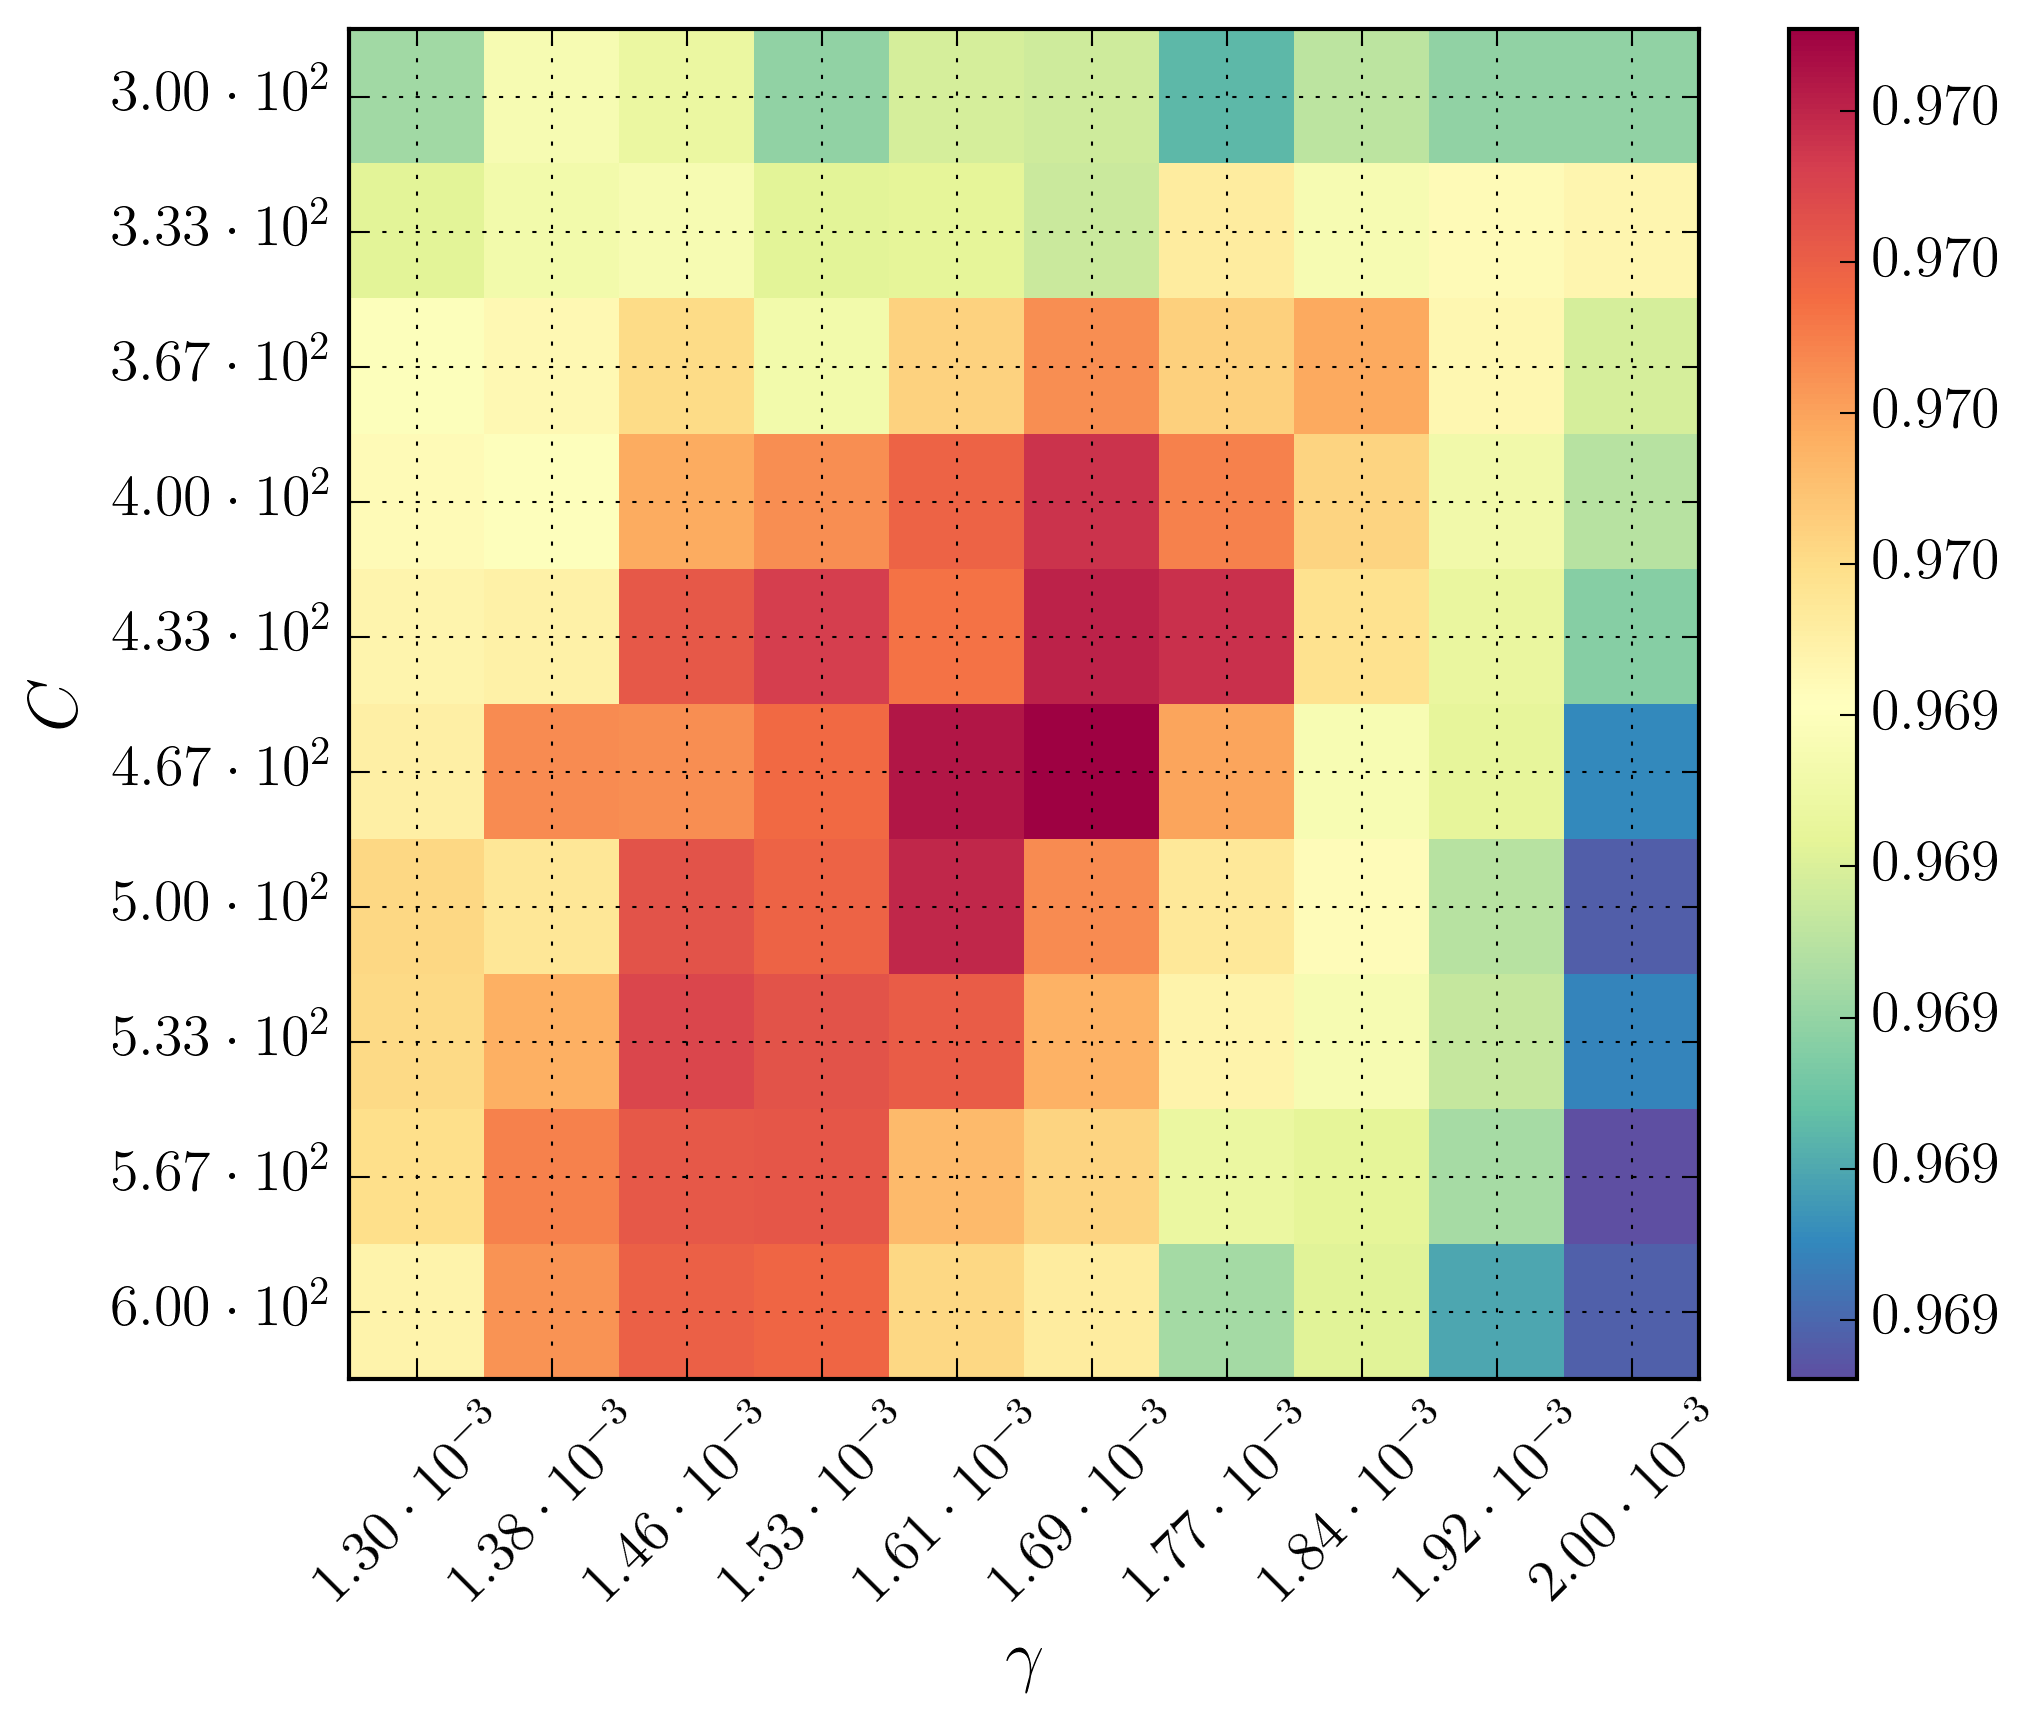
\includegraphics[width=\textwidth]{figures/gridsearch/svm/superclasses/svm-superclasses-06.png}
	\end{subfigure}
	\caption[Hyperparameter optimization for the Support Vector Machine (SVM)]{This figure shows the average, weighted $F_1$ score on the $C$-$\gamma$-plane during the hyperparameter optimization for the Support Vector Machine. We start looking for global optima on a coarse grid with a wide range (upper left), and adjust the grid toward a finer stepwidth. At some point we find an optimum (lower right).}
	\label{fig:gridsearch-svm-superclasses}
\end{figure}

\begin{landscape}
\begin{table}[ht!]
\centering
\resizebox{22cm}{!}{
\begin{tabular}{C{3.1cm}|C{.95cm}C{.95cm}C{.95cm}C{.95cm}C{.95cm}C{.95cm}C{.95cm}C{.95cm}C{.95cm}C{.95cm}C{.95cm}C{.95cm}C{.95cm}C{.95cm}C{.95cm}C{.95cm}C{.95cm}C{.95cm}C{.95cm}C{.95cm}C{.95cm}C{.95cm}C{.95cm}C{.95cm}C{.95cm}|c}
\toprule
 & \rot{BV} &   \rot{1O} &   \rot{F} &   \rot{CEPH Other} &   \rot{DSCT} &    \rot{EC} &    \rot{ED} &   \rot{ED ESD} &   \rot{ESD} &   \rot{EB Other} &   \rot{Mira AGB C} &   \rot{Mira AGB O} &   \rot{OSARG AGB C} &   \rot{OSARG AGB O} &   \rot{OSARG RGB C} &   \rot{OSARG RGB O} &   \rot{SRV AGB C} &   \rot{SRV AGB O} &   \rot{None\-Var} &   \rot{QSO} &   \rot{RRab} &   \rot{RRc} &   \rot{RRd} &   \rot{RRe} &   \rot{T2\-CEPH} &    $\Sigma$ \\
\midrule
BV & \bfseries 766      &     1     &           &              &          &   4      &    2      &             &   2      &     1      &                  &                  &                   &                   &                   &                   &                 &                 &     17      &   2      &            &           &           &           &     1      & 796  \\
1O &   2      &   \bfseries 723     &   51      &      24      &          &   5      &    2      &             &   5      &     2      &                  &                  &            1      &                   &                   &                   &                 &          2      &      2      &          &     9      &   10      &           &           &     6      & 844 \\
F &   1      &    98     & \bfseries 1162      &       4      &          &          &           &             &   1      &            &           1      &                  &                   &                   &                   &                   &                 &          1      &             &          &     3      &           &           &           &     4      & 1275 \\
CEPH Other &          &    34     &    3      &     \bfseries 	114      &          &   2      &           &             &   2      &            &                  &                  &                   &                   &                   &                   &                 &                 &             &          &     2      &    1      &    1      &           &     3      & 162 \\
DSCT &          &     1     &           &              & \bfseries 445      &   2      &    1      &      1      &   7      &     2      &                  &                  &                   &                   &                   &                   &                 &                 &     19      &          &     4      &   11      &    2      &   16      &            & 511 \\
EC &   1      &     8     &    1      &       1      &   4      & \bfseries 272      &    6      &      1      &  88      &    16      &                  &                  &            2      &                   &                   &           11      &                 &          1      &      4      &   1      &    13      &    3      &    2      &    5      &     5      & 445 \\
ED &   6      &     1     &           &       1      &   3      &  17      & \bfseries 1246      &     91      & 234      &    17      &                  &                  &            1      &            1      &                   &            1      &                 &                 &     24      &   1      &            &           &           &           &            & 1644 \\
ED ESD &          &           &           &              &   3      &   1      &   85      &    \bfseries 15      &  24      &     2      &                  &                  &                   &                   &                   &                   &                 &          1      &     14      &          &     1      &           &           &           &            & 146 \\
ESD &   9      &     4     &    1      &       1      &   2      & 140      &  204      &     35      & \bfseries 694      &    27      &                  &                  &                   &            3      &                   &           11      &                 &                 &      8      &          &     3      &    6      &           &    2      &            & 1150 \\
EB Other &   2      &     2     &           &              &   1      &  25      &   22      &      2      &  47      &    \bfseries 18      &                  &                  &            3      &            5      &                   &           10      &                 &                 &      9      &   2      &     3      &    1      &           &    1      &            & 153 \\
Mira AGB C &   1      &           &           &              &          &   1      &           &             &          &            &         \bfseries 689      &          15      &                   &                   &                   &            1      &         39      &          2      &      5      &   1      &            &           &           &           &            & 754 \\
Mira AGB O &          &           &           &              &          &          &           &             &          &            &          23      &        \bfseries 271      &                   &                   &                   &                   &          2      &         32      &      1      &          &            &           &           &           &            & 329 \\
OSARG	AGB C &   1      &           &           &              &          &          &           &             &          &            &           1      &                  &          \bfseries 958      &          206      &            5      &           13      &        198      &         15      &     19      &          &            &           &           &           &            & 1416 \\
OSARG AGB O &          &           &           &              &          &          &           &             &   1      &     4      &                  &                  &          388      &         \bfseries 2360      &            1      &          192      &         18      &        379      &     24      &          &     1      &           &           &           &            & 3368 \\
OSARG RGB C &          &           &           &              &          &          &           &             &          &            &           1      &                  &            8      &           11      &            \bfseries 6      &           20      &          6      &          2      &      2      &          &     1      &           &           &           &            & 57 \\
OSARG RGB O &   2      &           &    1      &              &          &  13      &    2      &             &   9      &     4      &           1      &                  &           22      &          149      &           21      &         \bfseries 1729      &          1      &         86      &      6      &          &            &           &           &           &            & 2046 \\
SRV AGB C &   1      &           &           &              &          &          &           &             &          &            &          93      &           2      &          301      &           18      &            3      &            4      &       \bfseries 3315      &         74      &      8      &          &            &           &           &           &            & 3819  \\
SRV AGB O &          &     1     &           &              &          &          &           &             &          &            &           7      &          72      &           58      &          329      &           15      &          136      &        106      &       \bfseries 3479      &      3      &          &            &           &           &           &            & 4206 \\
NonVar &  16      &           &           &              &  13      &   1      &   21      &      4      &  12      &     6      &           2      &                  &           20      &           34      &            4      &           14      &          1      &                 &   \bfseries 4613      &  28      &            &    1      &    1      &           &            & 4791 \\
QSO &   2      &           &           &              &          &   1      &           &             &   1      &            &           1      &                  &                   &                   &                   &                   &                 &                 &     33      & \bfseries 142      &            &           &           &           &            & 180 \\
RRab &          &    11     &    9      &       1      &   1      &  28      &           &             &  12      &     2      &                  &                  &                   &                   &            1      &                   &                 &                 &      9      &   1      &  \bfseries 3248      &   62      &   42      &    5      &     2      & 3434 \\
RRc &          &     5     &           &       2      &  11      &   5      &    3      &      1      &   6      &     4      &                  &                  &                   &                   &                   &                   &                 &                 &      2      &          &    46      &  \bfseries 574      &   23      &   32      &            & 714 \\
RRd &          &           &           &       1      &   1      &   4      &           &             &          &            &                  &                  &                   &                   &                   &                   &                 &                 &      1      &          &    42      &   40      &   \bfseries 89      &    1      &            & 179 \\
RRe &          &     1     &           &              &  22      &   4      &    1      &      1      &   4      &     1      &                  &                  &                   &                   &            1      &                   &                 &                 &             &          &     4      &   57      &    1      &   \bfseries 46      &            & 143 \\
T2CEPH &   1      &    16     &    4      &       5      &          &   8      &           &             &   5      &     3      &           2      &                  &                   &                   &                   &                   &          1      &          3      &      2      &          &    10      &           &           &           &    \bfseries 61      & 121 \\
\hline
Recall ($\%$) &   96.23 &    85.66 &   91.14 &       70.37 &   87.08 &   61.12 &   75.79 &      10.27 &    60.35 &     11.76 &           91.38 &           82.37 &            67.66 &            70.07 &            10.53 &             84.51 &          86.80 &          82.72 &      96.28 &  78.89 &     94.58 &    80.39 &    49.72 &    32.17 &     50.41 &        \\[.1cm]
\hline
Precision ($\%$) &      94.45 &     79.80 &    94.32 &       74.03 &   87.94 &   51.03 &    78.12 &      9.93 &   60.14 &     16.51 &           83.92 &           75.28 &            54.37 &            75.74 &            10.53 &            80.72 &          89.91 &          85.33 &      95.61 &   79.78 &     95.81 &    74.93 &    55.28 &    42.59 &     74.39 &        \\[.1cm]
\hline
$F_1$-score ($\%$) &   95.33 &    82.63 &   92.70 &       72.15 &   87.51 &   55.62 &   76.94 &      10.10 &    60.24 &     13.74 &           87.49 &           78.67 &            60.29 &            72.79 &           10.53 &             82.57 &          88.33 &          84.00 &      95.94 &  79.33 &     95.19 &   77.56  &  52.35   &  36.65   &     60.10 & $82.75 \pm 0.47$        \\[.1cm]
\bottomrule
\end{tabular}
}
\caption{This table shows the confusion matrix for the SVM subclasses classification on the EROS--2 data set with $C = 9.83 \cdot 10^{2}$ and $\gamma = 9.22 \cdot 10^{-4}$. The columns show the predicted labels, while the rows show the true label.}
\label{tab:svm-confusion-matrix-subclasses}
\end{table}
\end{landscape}

We then proceed to train the SVM for subclass classification\footnote{A complete list of the abbreviations used for the superclasses and subclasses can be found in the OGLE paper \citet{udalski2008}.}. Again, we optimize the hyperparameters $C$ and $\gamma$ using the same procedure as for the superclasses. The grid search results look fairly similar to figure \ref{fig:gridsearch-svm-superclasses}, so we don't include the individual results in the report. The optimal optimal hyperparameters for subclass classification are $C = 9.83 \cdot 10^{2}$ and $\gamma = 9.22 \cdot 10^{-4}$, leading to an average, weighted $F_1$-score of $(82.75 \, \pm \, 0.47) \, \%$.\\

\section{Performance of the Random Forest Classifier}
\label{sec:performance-rf}

The second classifier to evaluate is the Random Forest classifier. Once again, we optimize the model's hyperparameters $t$, the number of trees in the forest, and $m$, the maximum number of features to consider at each split. The individuals results on the grid can be inspected in figure \ref{fig:gridsearch-rf-superclasses}. It is clear to see that the scores are fluctuating on the finer grids, and we can not find one distinct optimum, but several local optima with a gradient in $t$. We discuss reasons for this in section \ref{sec:discussion}. Looking at the scores, we decide that $t = 1800$ and $m = 80$ seems like a justified choice. Table \ref{tab:rf-confusion-matrix-superclasses} shows the confusion matrix for the superclasses. The best average, weighted $F_1$-score is $(98.14 \, \pm \, 0.07) \, \%$.\\

\begin{figure}[h]
	\centering
	\begin{subfigure}[t]{0.49\textwidth}
		\centering
		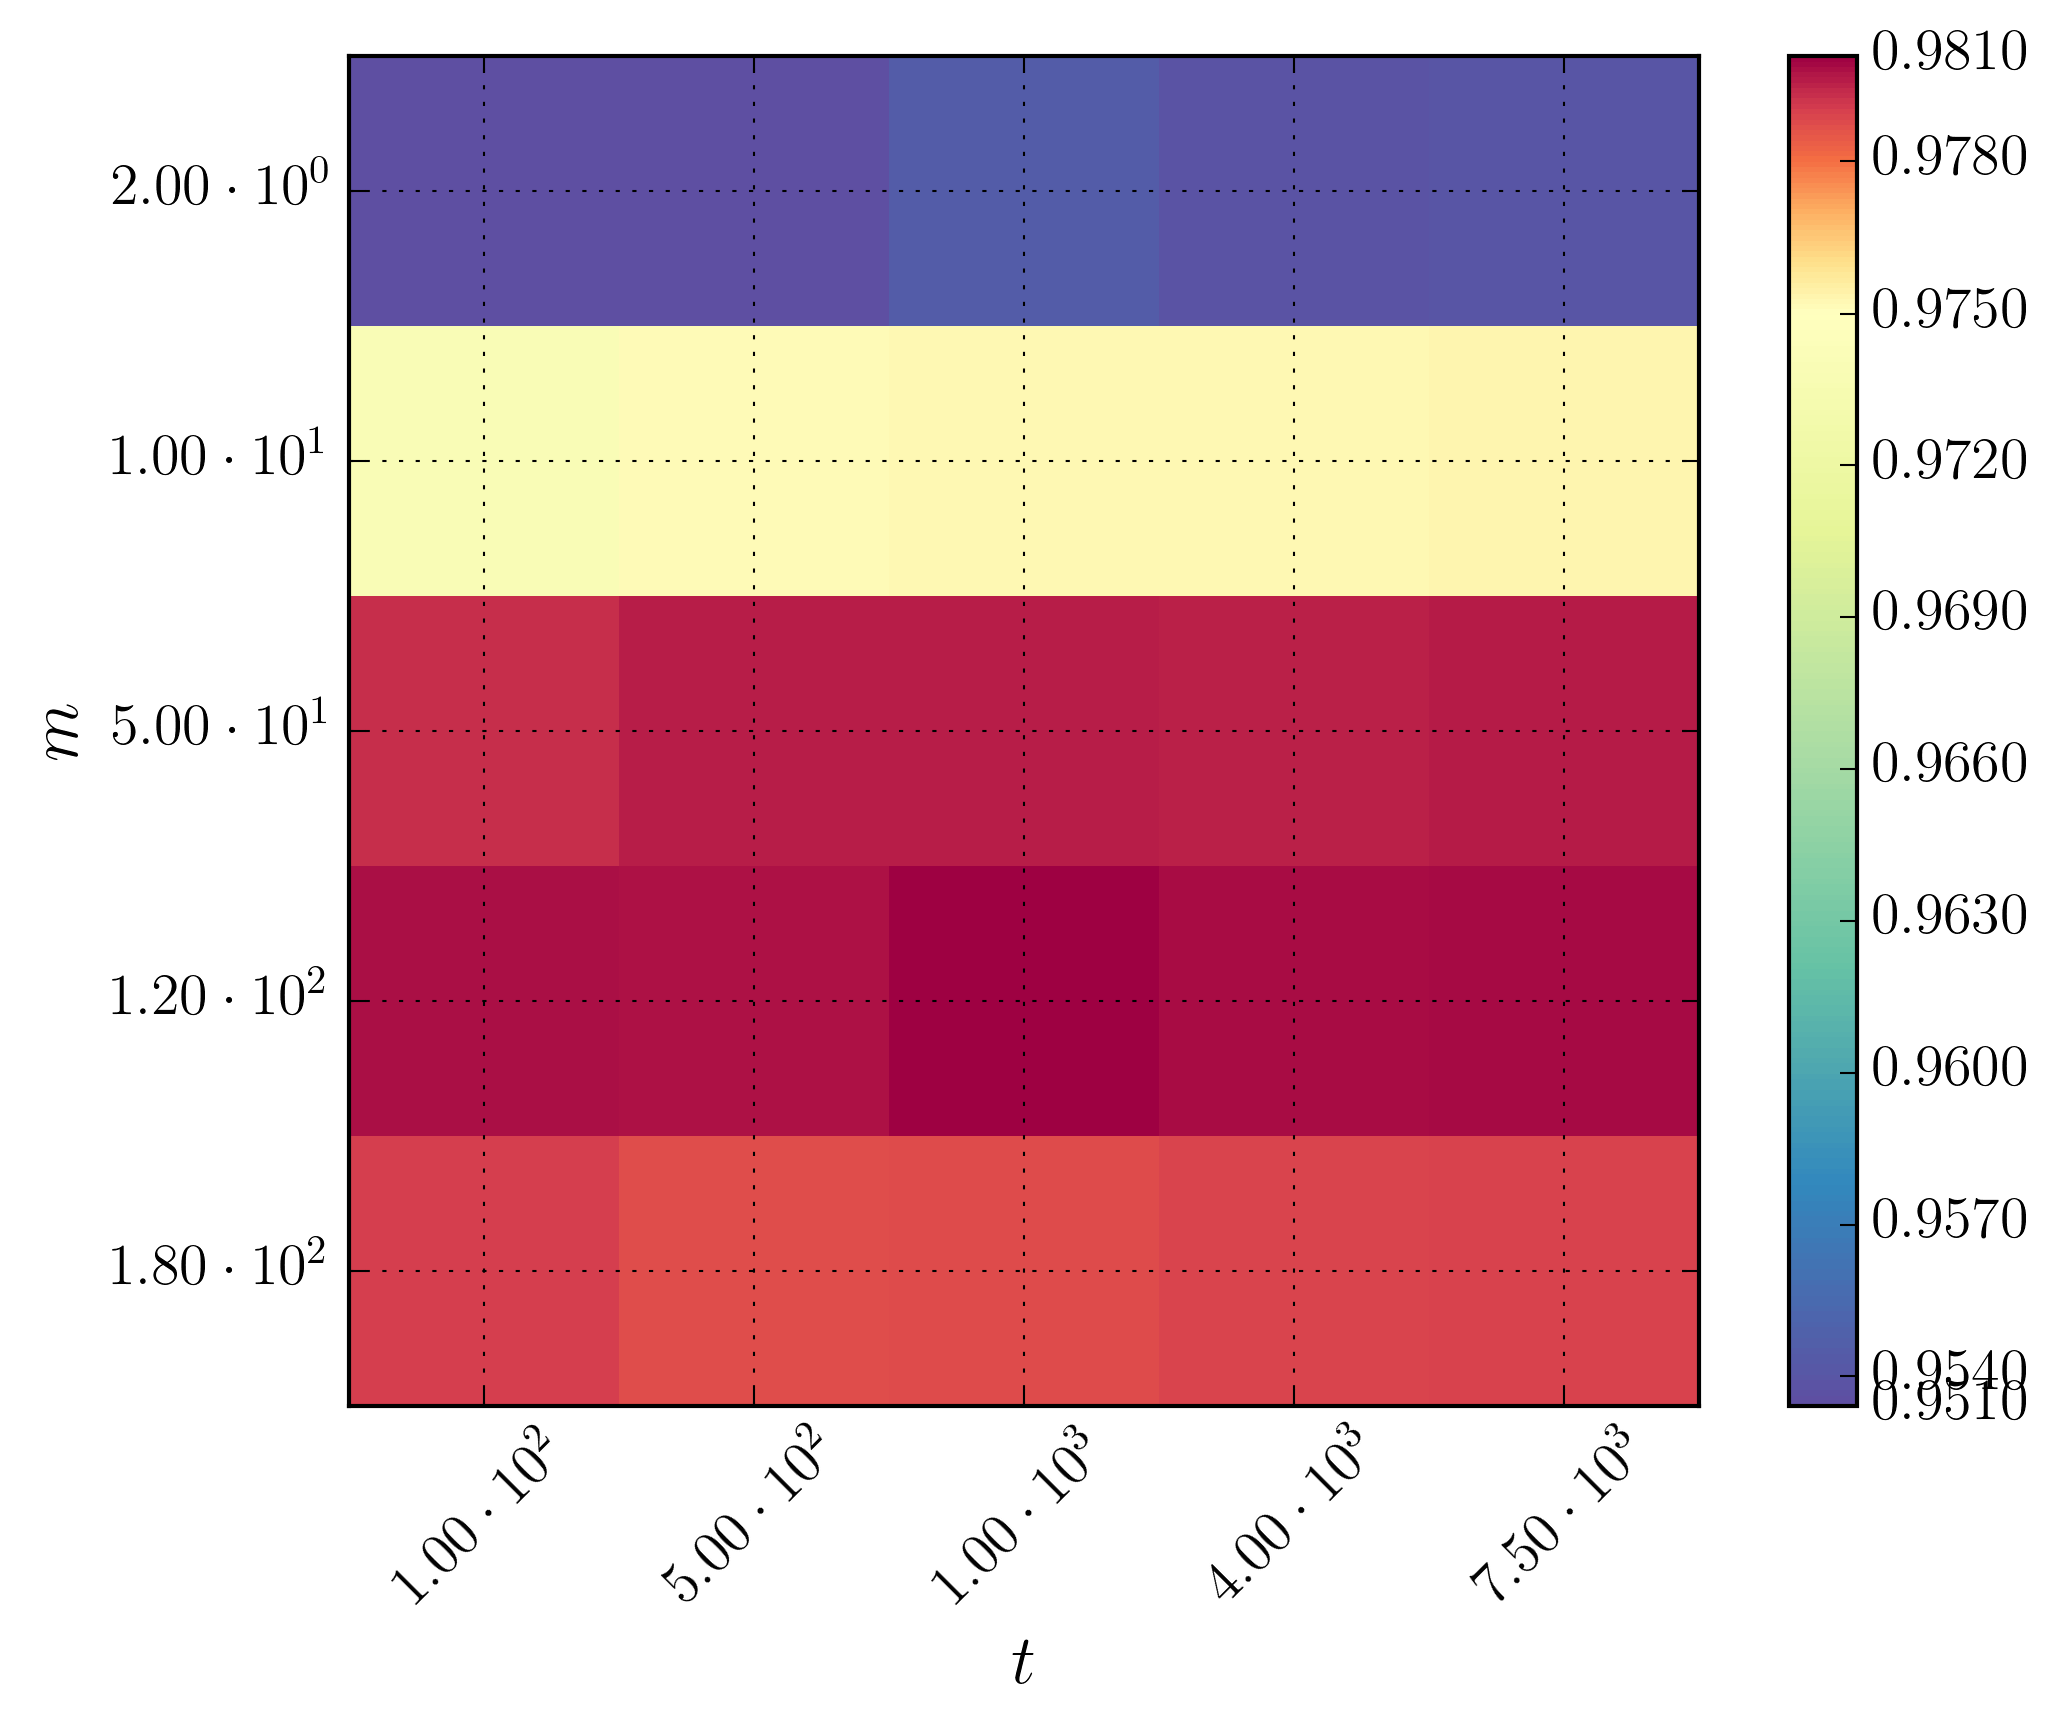
\includegraphics[width=\textwidth]{figures/gridsearch/rf/superclasses/rf-superclasses-01.png}
	\end{subfigure}
	\begin{subfigure}[t]{0.49\textwidth}
		\centering
		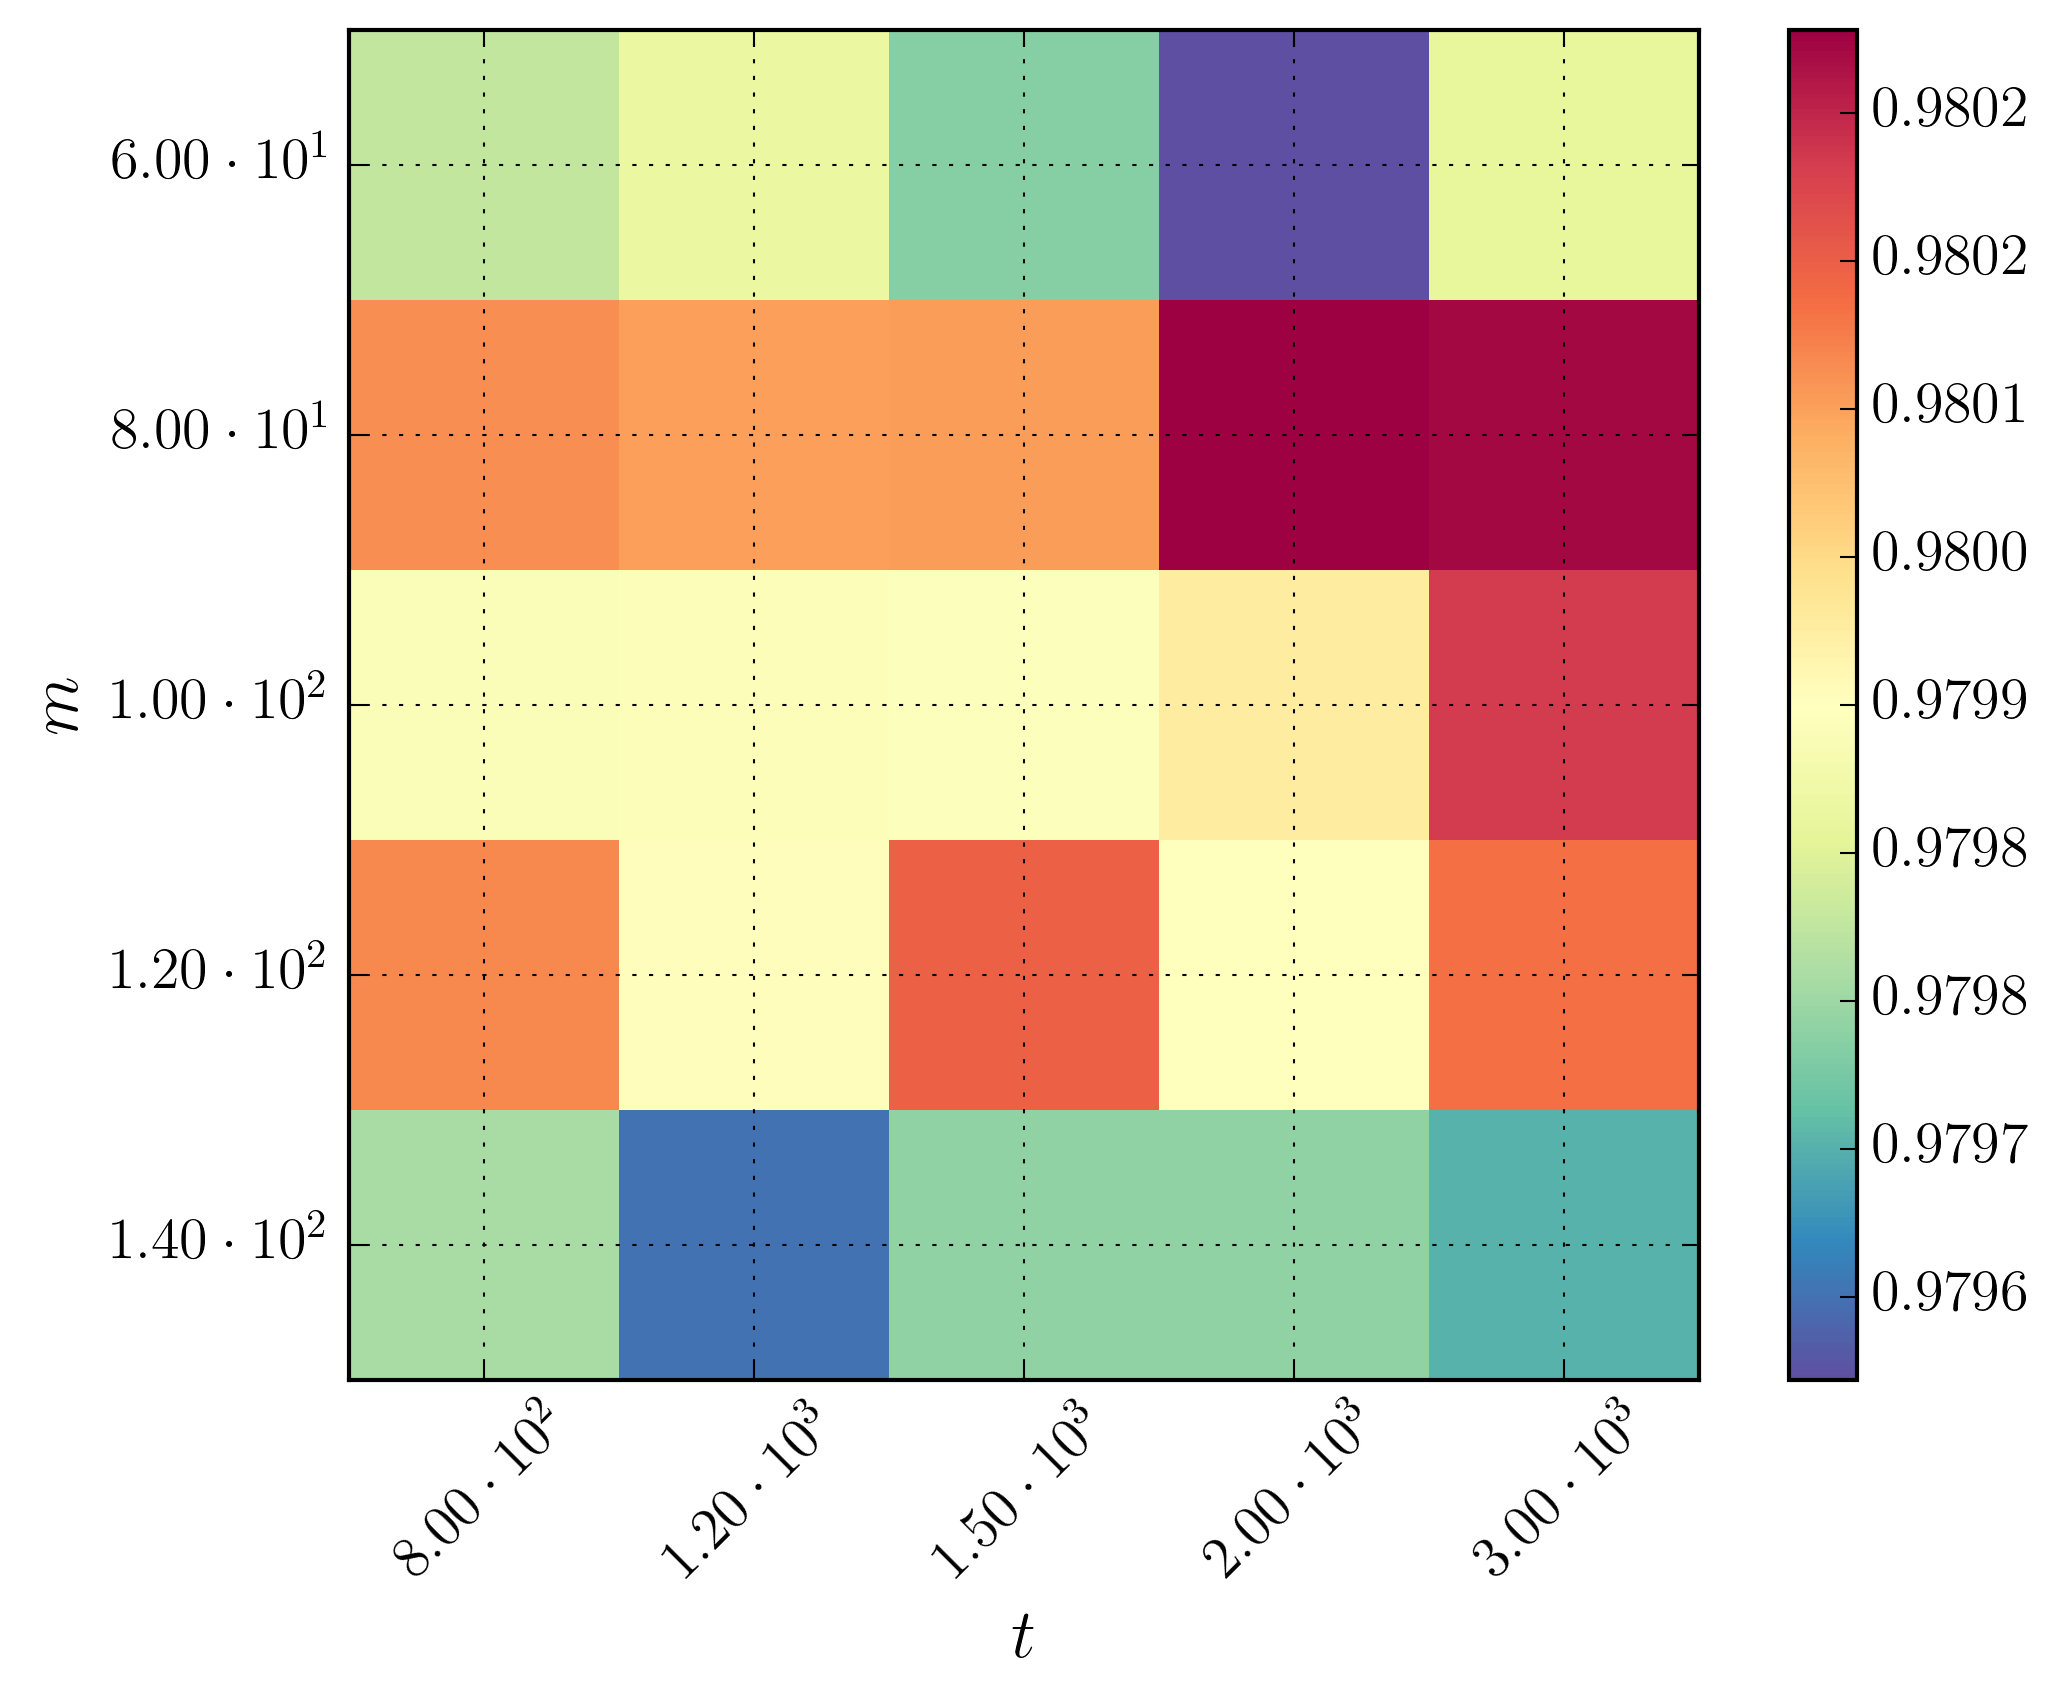
\includegraphics[width=\textwidth]{figures/gridsearch/rf/superclasses/rf-superclasses-02.png}
	\end{subfigure}
\end{figure}
\begin{figure}[h]
\ContinuedFloat
	\centering
	\begin{subfigure}[t]{0.49\textwidth}
		\centering
		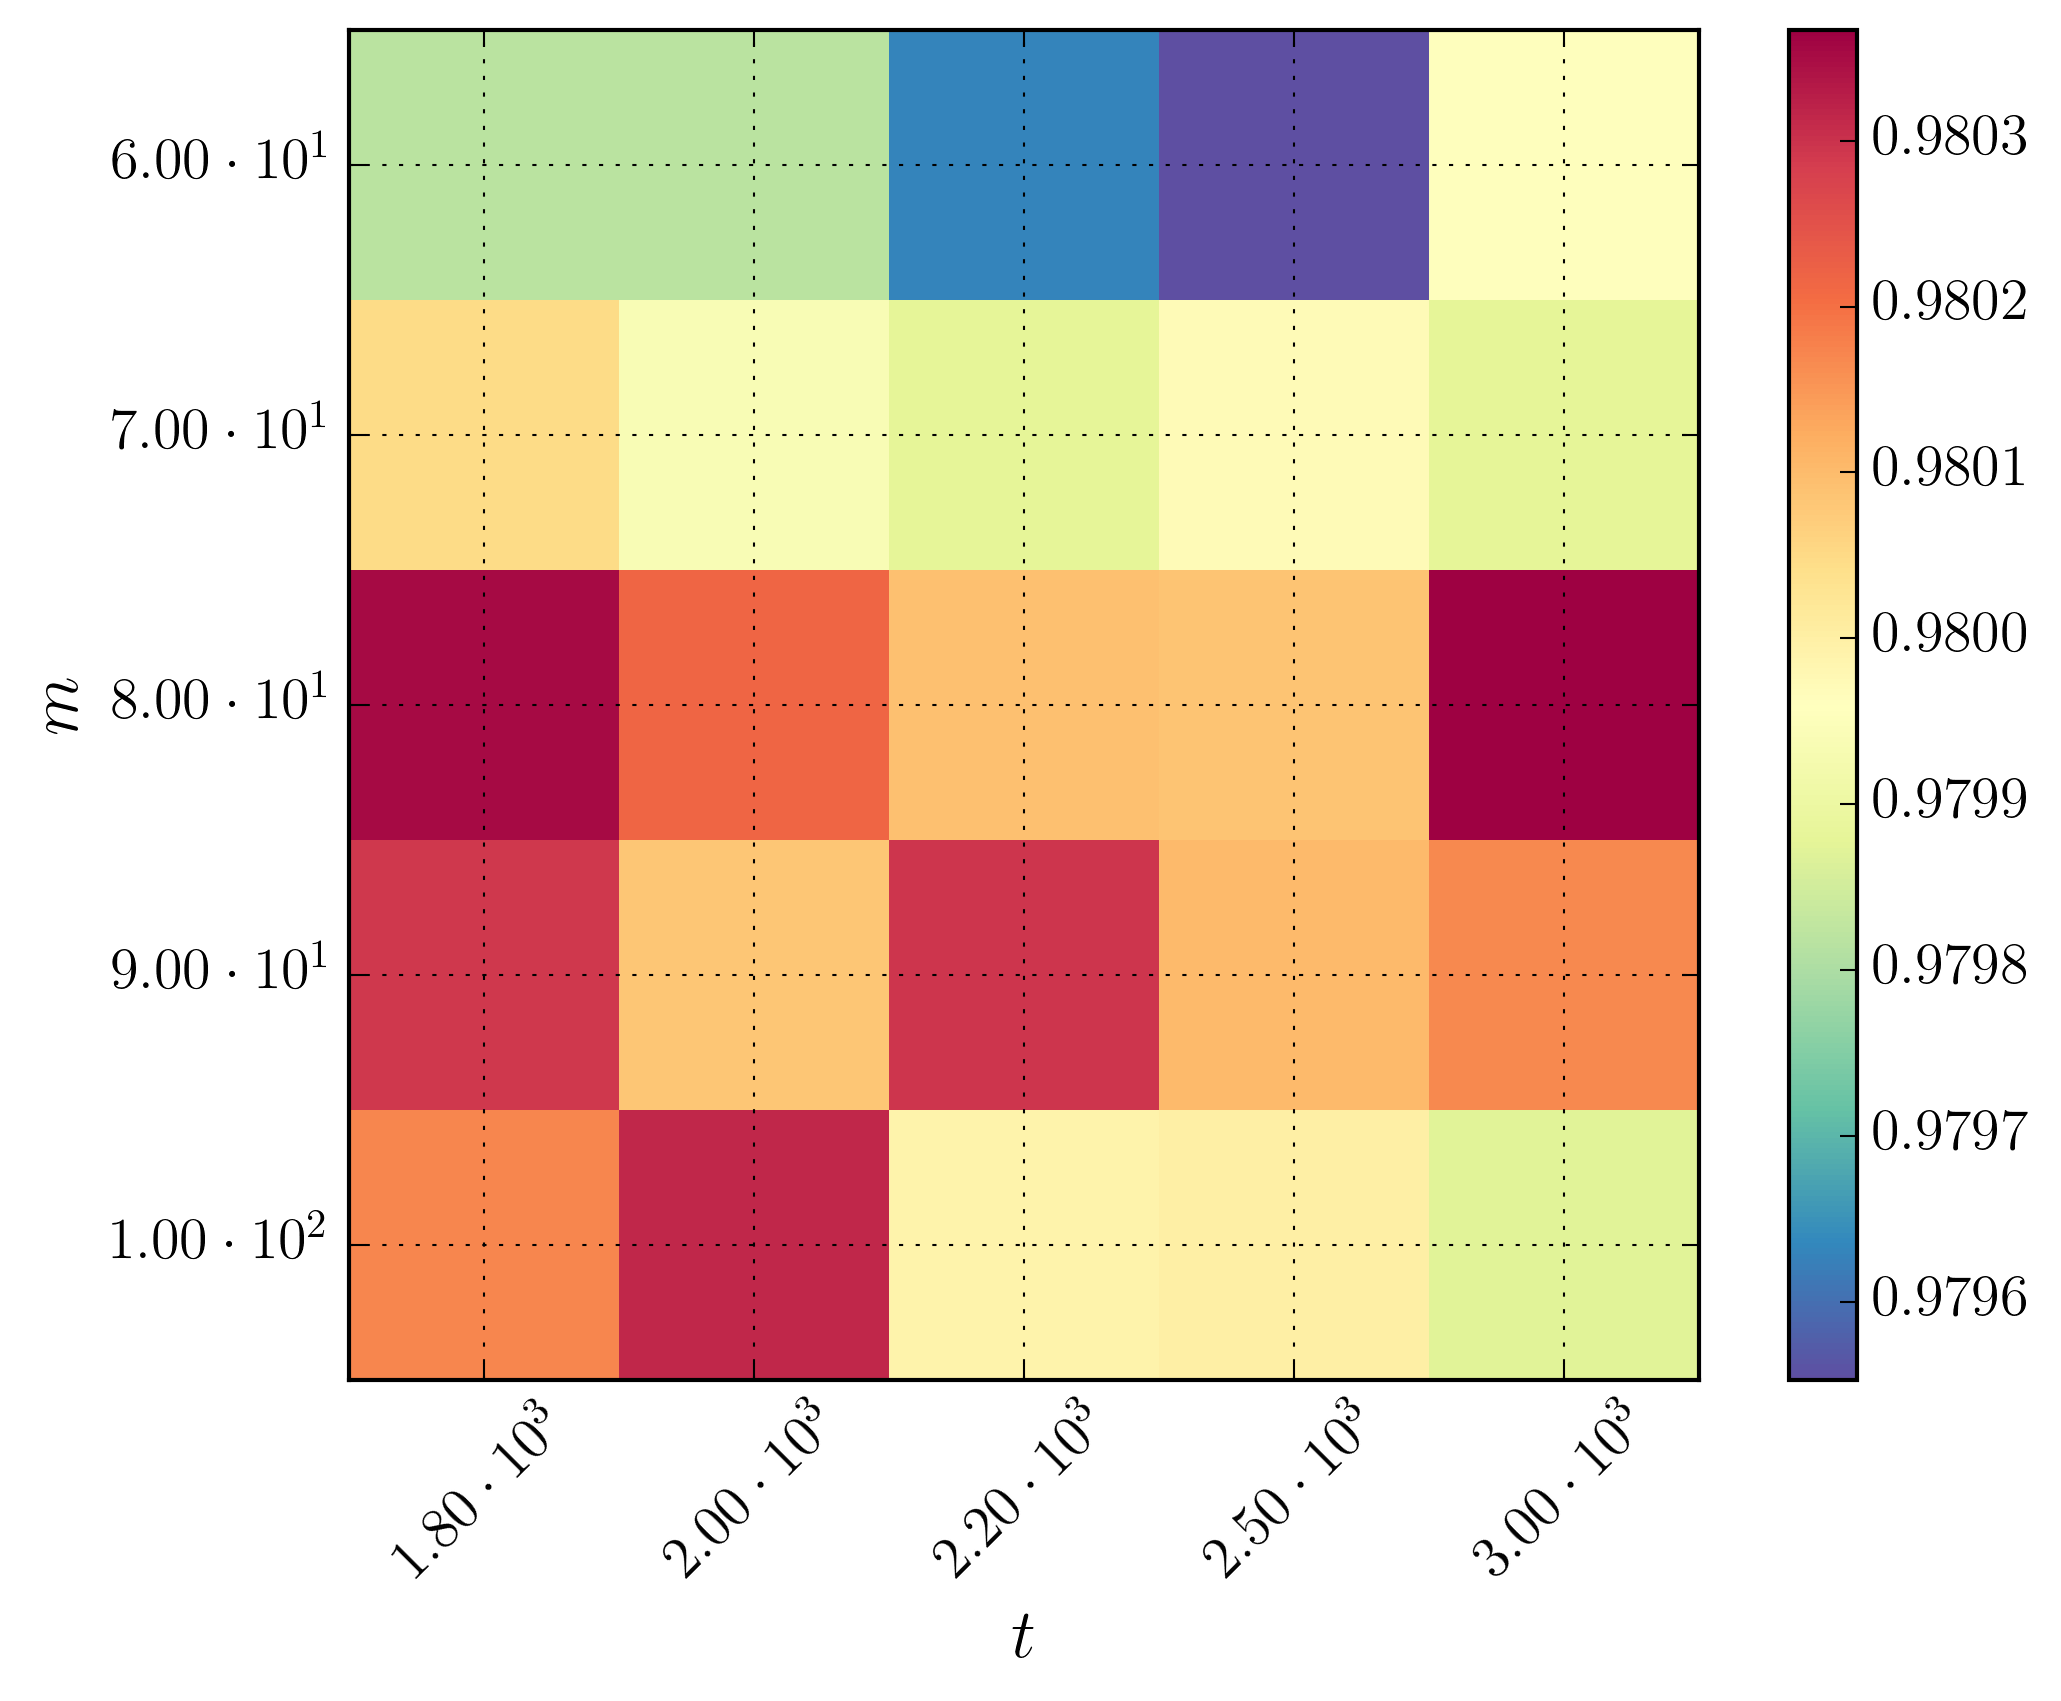
\includegraphics[width=\textwidth]{figures/gridsearch/rf/superclasses/rf-superclasses-03.png}
	\end{subfigure}
	\begin{subfigure}[t]{0.49\textwidth}
		\centering
		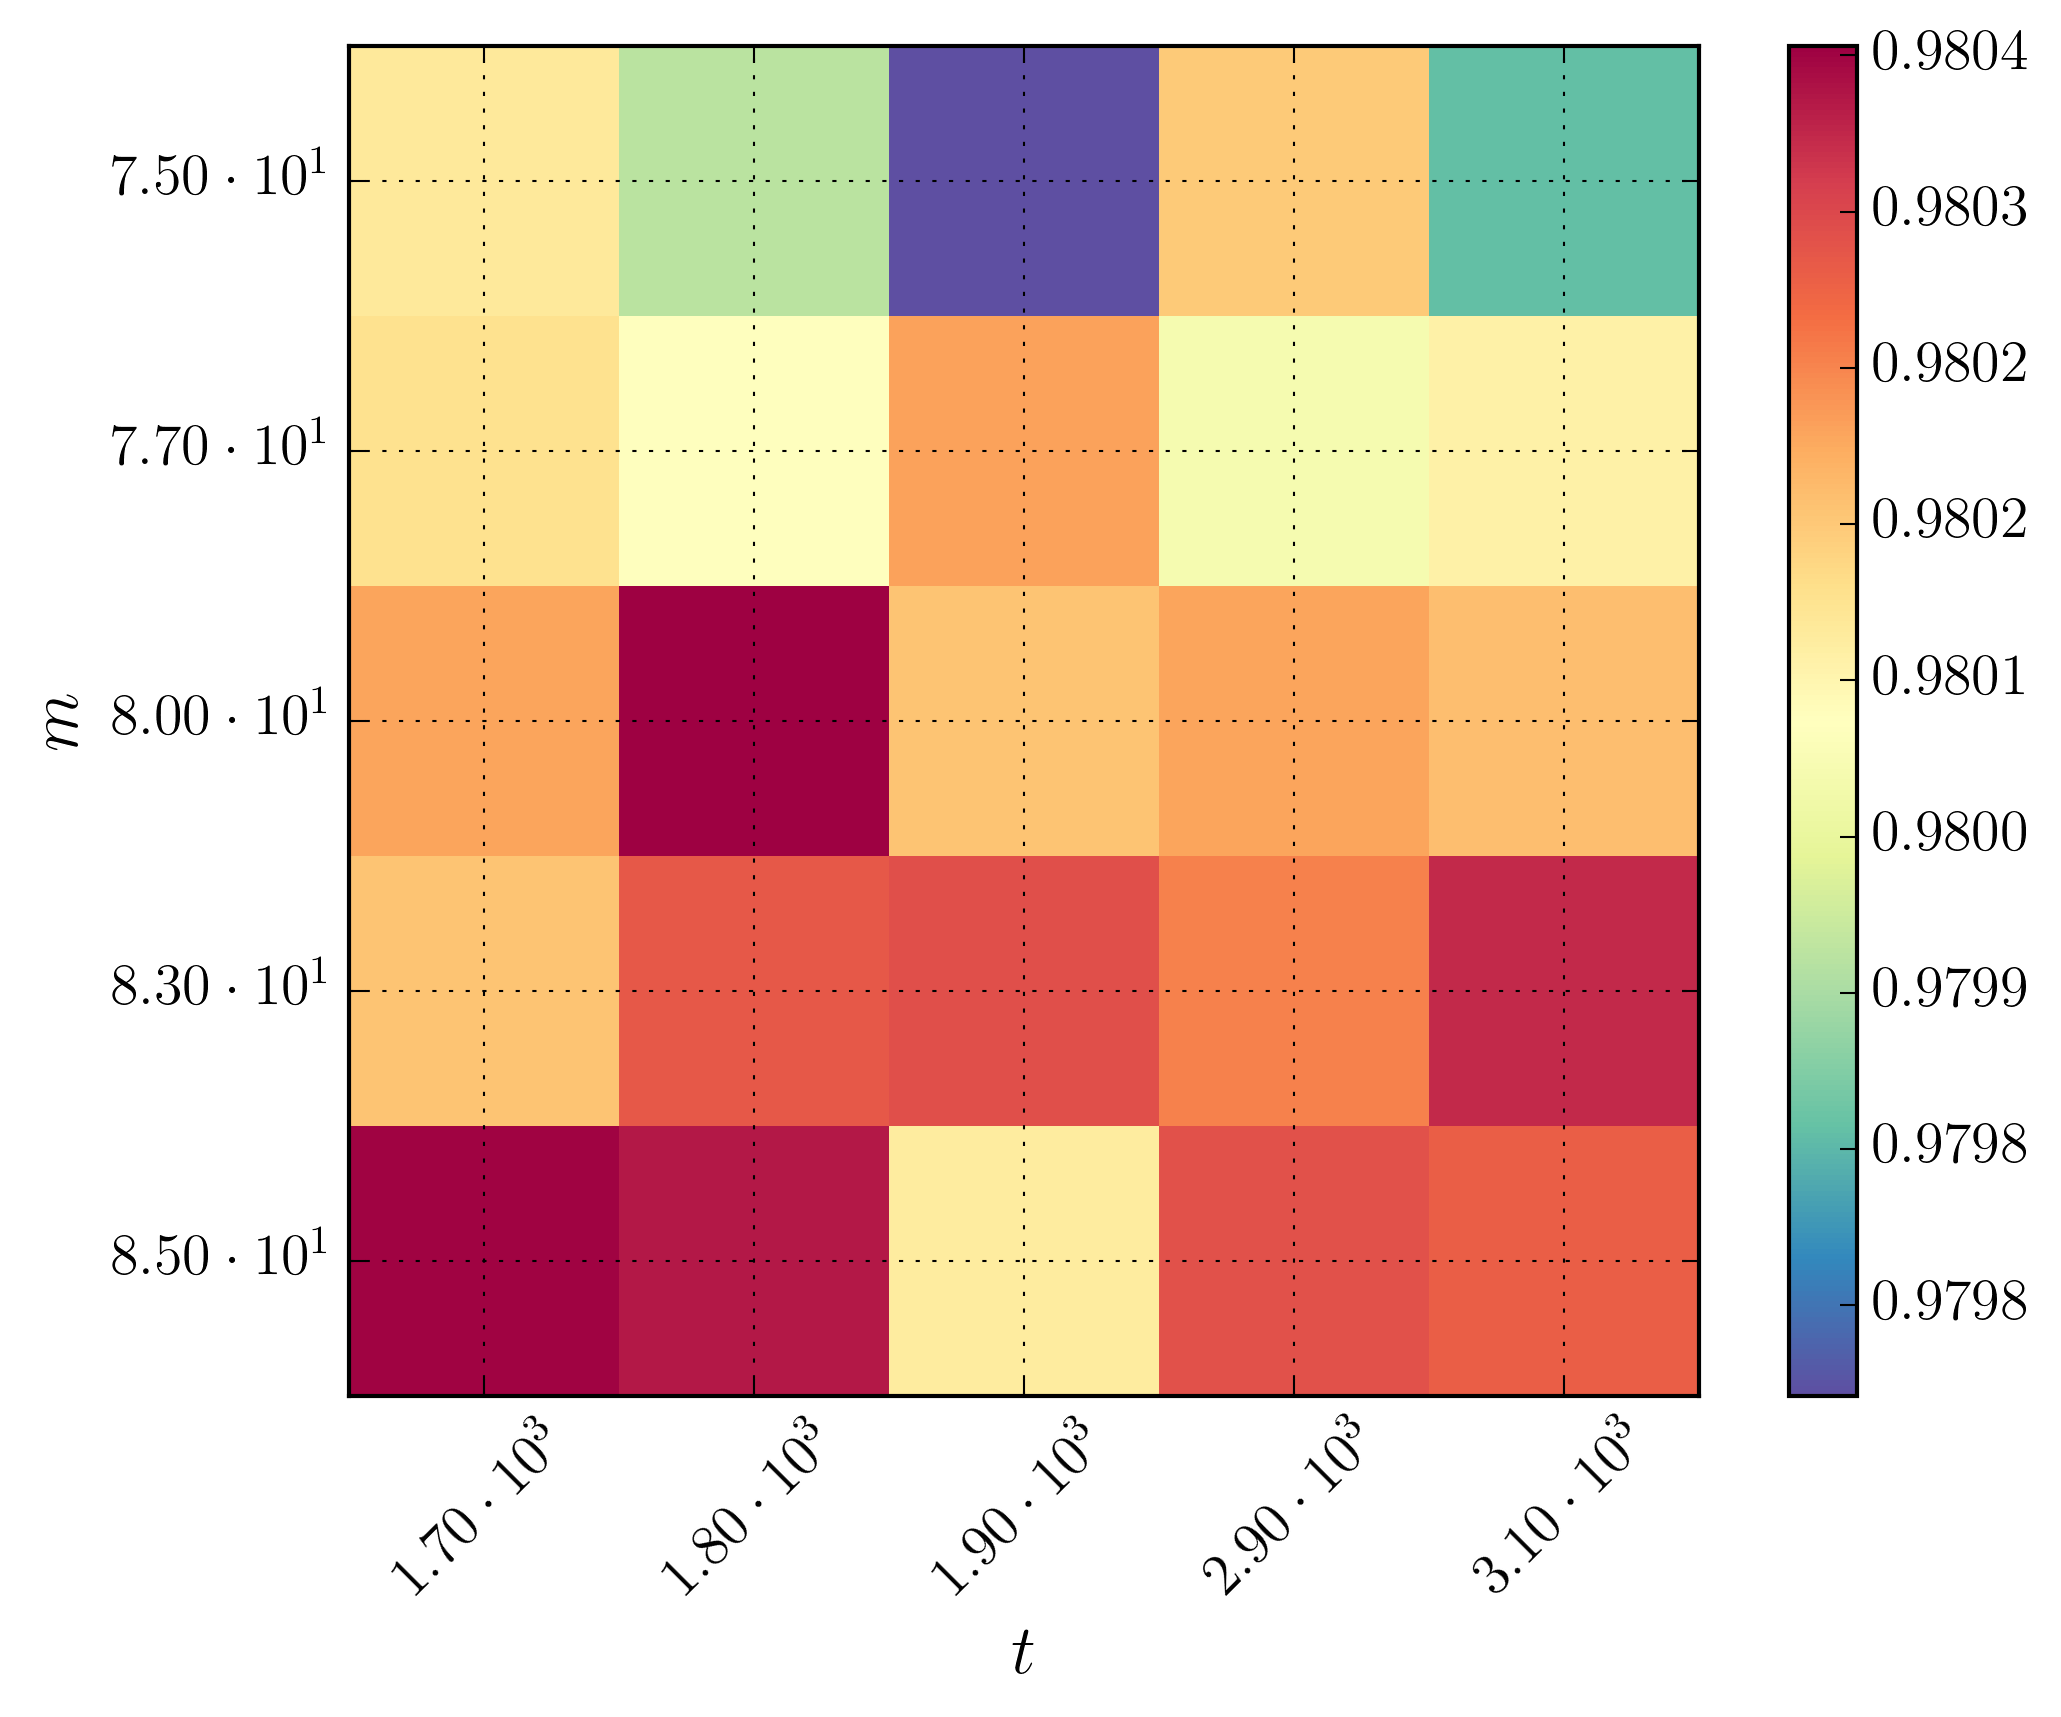
\includegraphics[width=\textwidth]{figures/gridsearch/rf/superclasses/rf-superclasses-04.png}
	\end{subfigure}
	\caption[Hyperparameter optimization for the Random Forest Classifier]{This figure shows the average, weighted $F_1$ score on the $m$-$t$-plane during the hyperparameter optimization for the Random Forest Classifier, where $t$ is the number of trees in the forest, and $m$ denotes the maximum number of features considered at each split.}
	\label{fig:gridsearch-rf-superclasses}
\end{figure}

\begin{figure}[H]
	\centering
	\begin{subfigure}[t]{\textwidth}
		\centering
		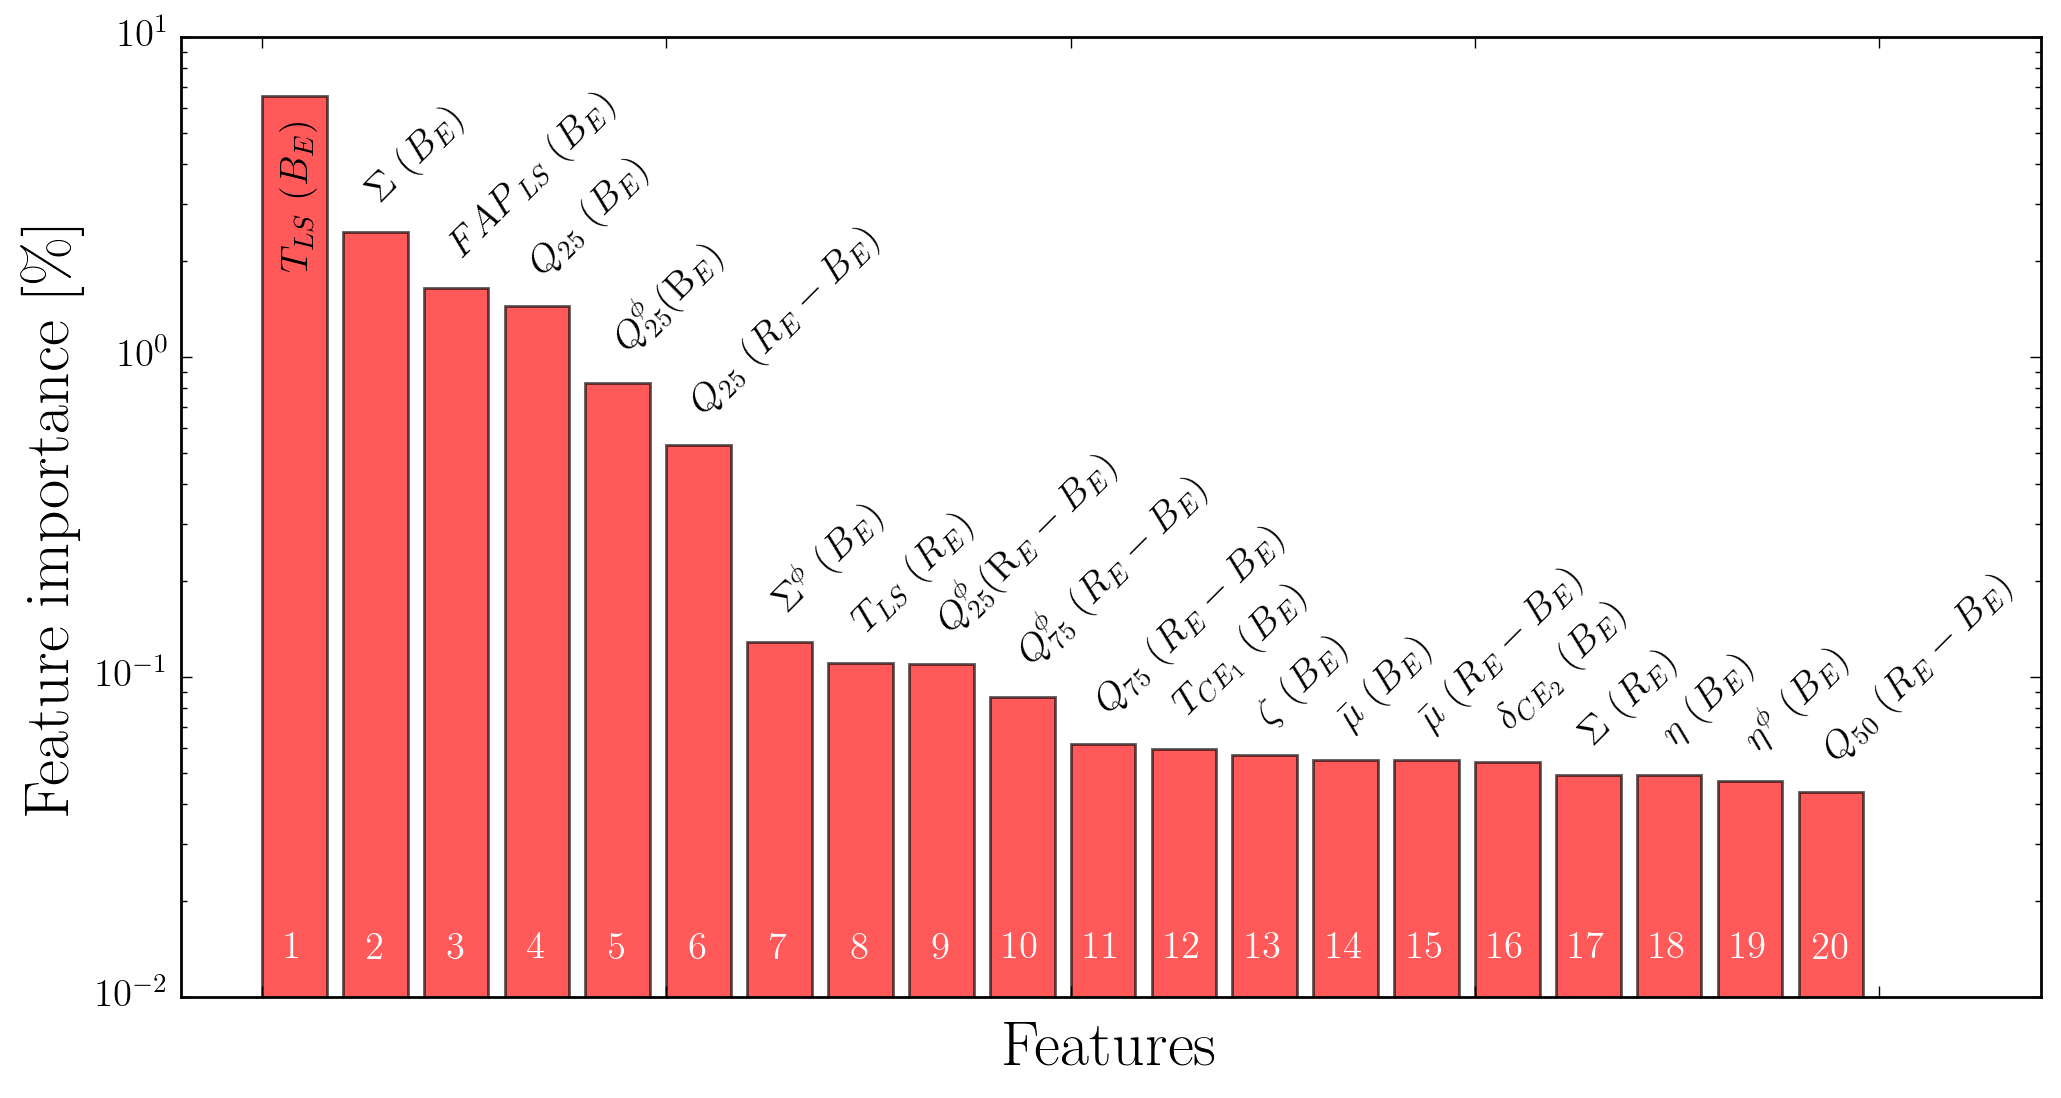
\includegraphics[width=\textwidth]{figures/feature-importance/rf-superclasses-feature-importance.png}
	\end{subfigure}
	\caption[Feature importance from the Random Forest classifier]{This figure shows the Random Forest feature importance ranking for the 20 best features during superclass classification. Note that the $y$-axis is in logarithmic scale. We can see that the the Lomb--Scargle period $T_\text{LS}$ is the most important feature by far.}
	\label{fig:rf-feature-importance}
\end{figure}

In figure \ref{fig:rf-feature-importance} we can see the feature importance ranking of the Random Forest algorithm for superclass classification. It is generated by averaging the normalized differences of the \emph{out--of--bag error} between a normal Random Forest models and a second model with \emph{randomly permuted} values of one feature over all trees \citep{dubath2011}. This could serve as a starting point as estimates for the feature importance, although one has to be very careful with this because it does not take feature correlations into account.\\

\begin{table}[h]
\centering
\resizebox{\textwidth}{!}{
\begin{tabular}{c|ccccccccc|c}
\toprule
                   & BV        & CEPH       & DSCT      & EB         & LPV         & NonVar    & QSO       & RRL        & T2CEPH   & $\Sigma $ \\
\midrule
BV                 & {\bfseries 773} &            &           &     11     &      3      &      8     &      1    &            &          &     796   \\
CEPH               &     1     & {\bfseries 2226} &           &     18     &      2      &      3     &           &     31     &          &    2281   \\
DSCT               &           &            & {\bfseries 496} &      2     &             &     12     &           &      1     &          &     511   \\
EB                 &     7     &      7     &     2     & {\bfseries 3342} &     52      &     79     &      3    &     43     &     3    &    3538   \\
LPV                &     4     &      2     &           &     10     & {\bfseries 15945} &     32     &      1    &     1      &          &   15995   \\
NonVar             &    23     &      1     &     4     &     35     &     72      & {\bfseries 4648} &      8    &            &          &    4791   \\
QSO                &           &            &           &      3     &      4      &     25     & {\bfseries 147} &     1      &          &     180   \\
RRL                &           &      9     &     7     &     31     &      2      &     7      &           & {\bfseries 4414} &          &    4470   \\
T2CEPH             &     1     &      15    &           &     19     &      5      &     3      &           &            & {\bfseries 78} &     121   \\
\bottomrule
Recall ($\%$)      &   97.11   &     97.59  &   97.06   &    94.46   &    99.69    &   97.02    &   81.67   &    98.75   &   64.46  &           \\
\hline
Precision ($\%$)   &   95.55   &     98.50  &   97.45   &    96.28   &    99.13    &   96.49    &   91.87   &    98.29   &   96.93  &           \\
\hline
$F_1$ score ($\%$) &   96.32   &     98.04  &   97.25   &    95.36   &    99.41    &   96.75    &   86.47   &    98.52   &   77.43  & 98.14 $\pm$ 0.07 \\
\bottomrule
\end{tabular}
}
\caption{This table shows the confusion matrix for the Random Forest superclasses classification on the EROS--2 data set with $m = 80$ and $t = 1800$. The columns show the predicted labels, while the rows show the true label.}
\label{tab:rf-confusion-matrix-superclasses}
\end{table}

\begin{table}[hb!]
\centering
\resizebox{0.7\textwidth}{!}{
\begin{tabular}{C{3cm}|C{3cm}C{3cm}|C{3cm}}
\toprule
 & Others  & QSO & $\Sigma $ \\
\midrule
Others & \bfseries 32501 & 2              & 32503 \\
QSO    &           97    & \bfseries   83 & 180 \\
\bottomrule
Recall ($\%$)      &   99.99 & 46.11 & \\
\hline
Precision ($\%$)   &   99.70 & 97.65 & \\
\bottomrule
\end{tabular}
}
\caption{This table shows the confusion matrix for a Random Forest classifier trying to separate quasars from other sources. It uses $t = 3000, m = 5$ and was optimized for quasar precision, minimizing contamination. It manages to identify 83 out of 180 quasars in the data set among 32503 other sources.}
\label{tab:rf-confusion-matrix-qso}
\end{table}

Futhermore, we trained the Random Forest classifier to do subclass classification. We settle for the hyperparameters $t = 1000, m = 100$, which leads to an average, weighted $F_1$-score of $(85.39 \, \pm \, 0.46) \, \%$. The respective confusion matrix is shown in table \ref{tab:rf-confusion-matrix-subclasses}.

\begin{landscape}
\begin{table}[h]
\centering
\resizebox{22cm}{!}{
\begin{tabular}{C{3.1cm}|C{.95cm}C{.95cm}C{.95cm}C{.95cm}C{.95cm}C{.95cm}C{.95cm}C{.95cm}C{.95cm}C{.95cm}C{.95cm}C{.95cm}C{.95cm}C{.95cm}C{.95cm}C{.95cm}C{.95cm}C{.95cm}C{.95cm}C{.95cm}C{.95cm}C{.95cm}C{.95cm}C{.95cm}C{.95cm}|c}
\toprule
 & \rot{BV} &   \rot{1O} &   \rot{F} &   \rot{CEPH Other} &   \rot{DSCT} &    \rot{EC} &    \rot{ED} &   \rot{ED ESD} &   \rot{ESD} &   \rot{EB Other} &   \rot{Mira AGB C} &   \rot{Mira AGB O} &   \rot{OSARG AGB C} &   \rot{OSARG AGB O} &   \rot{OSARG RGB C} &   \rot{OSARG RGB O} &   \rot{SRV AGB C} &   \rot{SRV AGB O} &   \rot{None\-Var} &   \rot{QSO} &   \rot{RRab} &   \rot{RRc} &   \rot{RRd} &   \rot{RRe} &   \rot{T2\-CEPH} &    $\Sigma$ \\
\midrule
BV          & \bfseries 777      &           &           &              &          &   2      &    2      &             &   4      &            &                  &                  &                   &                   &                   &                   &                 &                 &     10      &   1      &            &           &           &           &            & 796 \\
1O          &          &  \bfseries 764      &   23      &         18   &          &   2      &           &             &   4      &            &                  &                  &                   &                   &                   &                   &                 &                 &      8      &          &     7      &   13      &    1      &    4      &            & 844 \\
F           &   1      &   22      & \bfseries 1243      &          4   &          &          &           &             &   1      &            &                  &                  &                   &                   &                   &            1      &           1     &          1      &             &          &            &           &           &           &     1      & 1275 \\
CEPH Other  &          &   33      &    4      &        \bfseries 108   &          &          &           &             &   2      &            &                  &                  &                   &                   &                   &                   &                 &                 &      1      &          &     9      &    4      &           &           &     1      & 162 \\
DSCT        &          &           &           &              & \bfseries 492      &          &           &             &          &            &                  &                  &                   &                   &                   &                   &                 &                 &     14      &          &            &           &           &    5      &            & 511 \\
EC          &          &    1      &           &          1   &   3      & \bfseries 211      &   21      &             & 139      &     5      &                  &                  &                   &                   &                   &           15      &           2     &          2      &     11      &          &    10      &   17      &    1      &    3      &     3      & 445 \\
ED          &   2      &    1      &           &              &          &   6      & \bfseries 1427      &             & 142      &     1      &                  &                  &            1      &                   &                   &            1      &                 &                 &     50      &          &     8      &    4      &           &           &     1      & 1644  \\
ED ESD      &          &           &           &              &          &          &  112      &             &  13      &            &                  &                  &                   &                   &                   &                   &                 &                 &     21      &          &            &           &           &           &            & 146   \\
ESD         &   3      &    1      &    2      &              &   1      &  51      &  312      &             & \bfseries 703      &    10      &                  &                  &                   &                   &                   &           13      &                 &                 &     23      &   1      &    17      &   12      &           &    1      &            & 1150 \\
EB Other    &   1      &           &           &              &   2      &  14      &   33      &             &  57      &     \bfseries 5      &                  &                  &                   &            1      &                   &           12      &                 &                 &     26      &   1      &            &    1      &           &           &            & 153 \\
Mira AGB C  &          &           &           &              &          &          &           &             &   1      &            &         \bfseries 690      &           5      &                   &                   &                   &            3      &          48     &          5      &             &   2      &            &           &           &           &            & 754 \\
Mira AGB O  &          &           &           &              &          &          &           &             &          &            &          16      &        \bfseries 265      &                   &                   &                   &                   &           3     &         45      &             &          &            &           &           &           &            & 329 \\
OSARG AGB C &          &    1      &           &              &          &          &           &             &          &            &                  &                  &         \bfseries 777      &          286      &                   &           34      &         300     &         17      &      1      &          &            &           &           &           &            & 1416 \\
OSARG AGB O &          &           &           &              &          &          &           &             &   1      &            &                  &                  &          180      &         \bfseries 2606      &                   &          152      &          29     &        379      &     21      &          &            &           &           &           &            & 3368 \\
OSARG RGB C &          &           &           &              &          &          &           &             &   1      &            &           1      &                  &                   &           13      &                   &           26      &           4     &          8      &      4      &          &            &           &           &           &            & 57   \\
OSARG RGB O &   2      &    1      &           &              &          &   3      &    1      &             &   2      &     1      &           1      &                  &            3      &          138      &                 1 &         \bfseries 1774      &           5     &        103      &     11      &          &            &           &           &           &            & 2046 \\
SRV AGB C   &   1      &           &           &              &          &          &           &             &          &            &          70      &                  &           85      &           27      &                   &           18      &        \bfseries 3502     &        112      &      3      &   1      &            &           &           &           &            & 3819  \\
SRV AGB O   &   1      &           &    1      &              &          &   1      &           &             &          &     1      &           1      &          18      &           19      &          356      &                   &          129      &         119     &       \bfseries 3551      &      4      &          &            &           &           &           &     5      & 4206 \\
NonVar     &  25      &           &           &              &   6      &   1      &   17      &             &   1      &            &                  &                  &            9      &           41      &                   &            5      &           2     &          2      &   \bfseries 4674      &   8      &            &           &           &           &            & 4791 \\
QSO         &          &           &           &              &          &          &    1      &             &          &            &                  &                  &                   &                   &                   &                   &           1     &                 &     27      & \bfseries 148      &     3      &           &           &           &            & 180 \\
RRab        &          &    1      &           &          2   &          &   2      &    7      &             &   9      &            &                  &                  &                   &            1      &                   &                   &                 &                 &     10      &          &  \bfseries 3398      &    2      &    2      &           &            & 3434 \\
RRc         &          &    1      &           &              &          &   2      &           &             &   3      &            &                  &                  &                   &                   &                   &                   &                 &                 &      3      &          &     3      &  \bfseries 666      &   11      &   25      &            & 714 \\
RRd         &          &           &           &          1   &          &          &           &             &          &            &                  &                  &                   &                   &                   &                   &                 &                 &      1      &          &     7      &   49      &  \bfseries 121      &           &            & 179  \\
RRe         &          &           &           &              &   4      &          &           &             &          &            &                  &                  &                   &                   &                   &            1      &                 &                 &      1      &          &     1      &   12      &           &  \bfseries 124      &            & 143 \\
T2CEPH      &          &    4      &   10      &          1   &          &   5      &    3      &             &  10      &            &                  &                  &                   &                   &                   &            1      &                 &          1      &      2      &          &     3      &           &           &           &    \bfseries 81      & 121 \\
\hline
Recall ($\%$) &   97.61 &    90.52 &   97.49 &       66.67 &   96.28 &   47.42 &   86.80 &      0.00 &    61.13 &     3.27 &           91.51 &           80.55 &            54.87 &            77.38 &            0.00 &             86.71 &          91.17 &          84.43 &      97.56 &  82.22 &     98.95 &    93.28 &    67.60 &    86.71 &     66.94 &        \\[.1cm]
\hline
Precision ($\%$) &         95.57 &    92.05 &    96.88 &          80.00 &   96.85 &   70.33 &    73.71 &         0.00 &   64.32 &     21.74 &           88.58 &           92.01 &            72.35 &            75.12 &         0.00          &            81.19 &           87.20 &          84.03 &      94.88 &   91.36 &     98.04 &    85.38 &    88.97 &    76.54 &     88.04 &        \\[.1cm]
\hline
$F_1$-score ($\%$) &   96.58 &    91.28 &   97.18 &       72.73 &   96.56 &   56.65 &   79.72 &      0.00 &    62.68 &     5.68 &           90.02 &           85.90 &            62.41 &            76.23 &           0.00 &             83.86 &          89.14 &          84.23 &      96.20 &  86.55 &     98.49 &   89.16  &  76.83   & 81.31   &     76.05 & $85.39 \pm 0.46$        \\[.1cm]
\bottomrule
\end{tabular}
}
\caption{This table shows the confusion matrix for the Random Forest subclasses classification on the EROS--2 data set. The columns show the predicted labels, while the rows show the true label.}
\label{tab:rf-confusion-matrix-subclasses}

\end{table}
\end{landscape}

\section{Performance of Gradient Boosted Trees}
\label{sec:performance-gb}

The third and last model we train is the Gradient Boosted classifier. In contrast to the previous two classifiers, we have three hyperparameters and a systematic way of finding the optimal combination is difficult. The hyperparameters are \emph{the number of trees}, \emph{number of features to use} and the \emph{learning rate}, where the latter controls the contribution of each iteration during boosting. However, we found that 10000 trees with 80 features and a learning rate of 0.02 provide decent results. Table \ref{tab:gb-confusion-matrix-superclasses} shows the confusion matrix for superclass classification, where we achieve an average, weighted $F_1$-score of $(98.43 \, \pm \, 0.07) \, \%$.\\

%\begin{figure}[H]
%	\centering
%	\begin{subfigure}[t]{\textwidth}
%		\centering
%		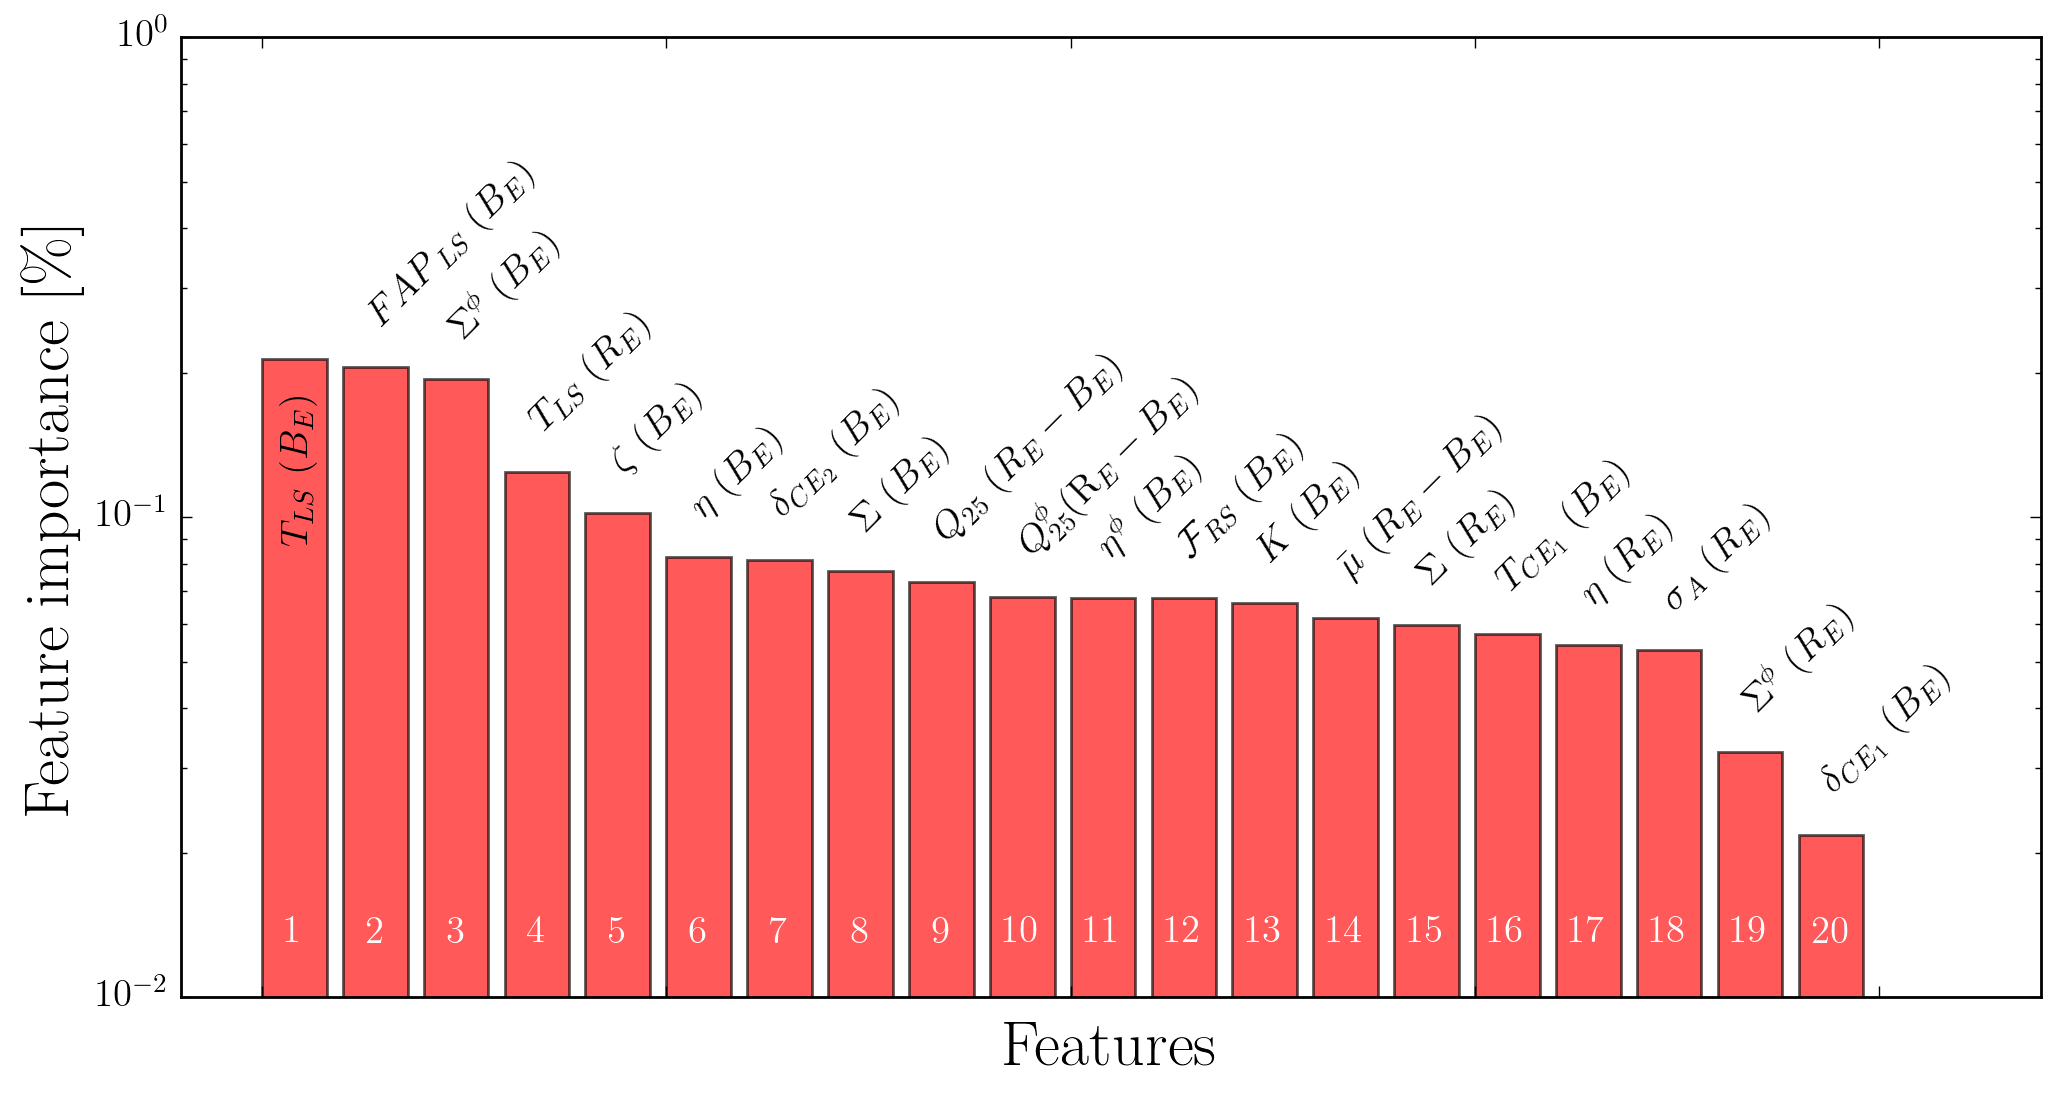
\includegraphics[width=\textwidth]{figures/feature-importance/gb-superclasses-feature-importance.png}
%	\end{subfigure}
%	\caption[Feature importance from the Gradient Boosted Trees Classifier]{This figure shows the Gradient Boosted Trees feature importance ranking for the 20 best features during supercl%ass classification. Note that the $y$-axis is in logarithmic scale.}
%	\label{fig:gb-feature-importance}
%\end{figure}

\begin{table}[h]
\centering
\resizebox{\textwidth}{!}{
\begin{tabular}{c|ccccccccc|c}
\toprule
                   & BV        & CEPH       & DSCT      & EB         & LPV         & NonVar    & QSO       & RRL        & T2CEPH   & $\Sigma $ \\
\midrule
BV                 & \bfseries 773     &           &          &    7      &     3      &   12      &          &          &   1      & 796   \\
CEPH               &   1     & \bfseries 2230      &          &    5      &     1      &    5      &          &   39     &          & 2281  \\
DSCT               &         &           & \bfseries 495      &           &            &   11      &          &    5     &          & 511   \\
EB                 &   5     &    5      &   4      & \bfseries 3402      &    47      &   50      &          &   25     &          & 3538  \\
LPV                &   4     &    2      &          &   16      & \bfseries 15945      &   26      &   1      &    1     &          & 15995 \\
NonVar             &  15     &    1      &   3      &   23      &    60      & \bfseries 4681      &   6      &    2     &          & 4791  \\
QSO                &   2     &           &          &    3      &            &   25      & \bfseries 150      &          &          & 180   \\
RRL                &         &    6      &   5      &   27      &     2      &    2      &          & \bfseries 4428     &          & 4470  \\
T2CEPH             &  1     &   17      &          &   22      &     7      &    1      &          &          &   \bfseries 73      & 121   \\
\bottomrule
Recall ($\%$)      &   97.11   &     97.76  &   96.87   &    96.16   &    99.69    &   97.70    &    83.33  &    99.06   &   60.33  &           \\
\hline
Precision ($\%$)   &   96.50   &     98.63  &   97.63   &    97.06   &    99.25    &   97.26    &    95.54  &    98.40   &   98.65  &           \\
\hline
$F_1$ score ($\%$) &   96.30   &     98.13  &   97.25   &    96.61   &    99.47    &   97.48    &    89.02  &    98.73   &   74.87  & 98.43 $\pm$ 0.07 \\
\bottomrule

\end{tabular}
}
\caption{This table shows the confusion matrix for the Gradient Boosted Classifier superclasses classification on the EROS--2 data set. The columns show the predicted labels, while the rows show the true label.}
\label{tab:gb-confusion-matrix-superclasses}
% 98.43% (+/-0.07%) for {'max_features': 80, 'n_estimators': 10000, 'learning_rate': 0.02, 'max_depth': 10, 'min_samples_leaf': 500}
\end{table}

The confusion matrix for subclass classification can be found in table \ref{tab:gb-confusion-matrix-subclasses}. For the subclasses, we used 6000 trees with 75 features and a learning rate of 0.01. The average, weighted $F_1$-score is $(86.30 \, \pm \, 0.37) \, \%$.

\begin{landscape}
\begin{table}[h]
\centering
\resizebox{22cm}{!}{
\begin{tabular}{C{3.1cm}|C{.95cm}C{.95cm}C{.95cm}C{.95cm}C{.95cm}C{.95cm}C{.95cm}C{.95cm}C{.95cm}C{.95cm}C{.95cm}C{.95cm}C{.95cm}C{.95cm}C{.95cm}C{.95cm}C{.95cm}C{.95cm}C{.95cm}C{.95cm}C{.95cm}C{.95cm}C{.95cm}C{.95cm}C{.95cm}|c}
\toprule
 & \rot{BV} &   \rot{1O} &   \rot{F} &   \rot{CEPH Other} &   \rot{DSCT} &    \rot{EC} &    \rot{ED} &   \rot{ED ESD} &   \rot{ESD} &   \rot{EB Other} &   \rot{Mira AGB C} &   \rot{Mira AGB O} &   \rot{OSARG AGB C} &   \rot{OSARG AGB O} &   \rot{OSARG RGB C} &   \rot{OSARG RGB O} &   \rot{SRV AGB C} &   \rot{SRV AGB O} &   \rot{None\-Var} &   \rot{QSO} &   \rot{RRab} &   \rot{RRc} &   \rot{RRd} &   \rot{RRe} &   \rot{T2\-CEPH} &    $\Sigma$ \\
\midrule
BV          & \bfseries 776      &           &           &              &          &          &    1      &             &   3      &     1      &                  &                  &                   &                   &                   &                   &          1      &          1      &      12     &   1      &            &           &           &           &            & 796 \\
1O          &          &  \bfseries 771      &   21      &      16      &          &   1      &    1      &             &   4      &            &                  &                  &                   &                   &                   &                   &                 &          2      &       4     &          &     5      &   14      &    1      &    4      &            & 844 \\
F           &   1      &   22      & \bfseries 1244      &       5      &          &          &           &             &          &            &            1     &                  &                   &            1      &                   &                   &                 &                 &             &          &            &           &           &           &     1      & 1275 \\
CEPH Other  &          &   40      &    5      &      \bfseries 97      &          &          &           &             &   2      &            &                  &                  &                   &                   &                   &                   &                 &                 &             &          &    14      &    4      &           &           &            & 162 \\
DSCT        &          &           &           &              & \bfseries 497      &          &           &             &          &            &                  &                  &                   &                   &                   &                   &                 &                 &      11     &          &            &           &           &    3      &            & 511 \\
EC          &          &    6      &    1      &              &   3      & \bfseries 205      &   20      &         1   & 156      &     9      &                  &                  &                   &                   &                   &           13      &          4      &          4      &       2     &          &     7      &    8      &    1      &    5      &            & 445 \\
ED          &   2      &           &           &              &          &   8      & \bfseries 1404      &         2   & 186      &     2      &                  &                  &                   &            1      &                   &            1      &          1      &                 &      32     &          &     2      &    2      &           &           &     1      & 1644  \\
ED ESD      &          &           &           &              &          &          &  113      &         \bfseries 1   &  16      &     1      &                  &                  &                   &                   &                   &                   &                 &                 &      15     &          &            &           &           &           &            & 146 \\
ESD         &   3      &    4      &    2      &              &          &  58      &  257      &         1   & \bfseries 762      &     7      &                  &                  &                   &            3      &                   &           14      &                 &          1      &      13     &          &    16      &    7      &    1      &    1      &            & 1150 \\
EB Other    &   3      &           &           &              &   1      &  20      &   31      &             &  56      &     \bfseries 7      &                  &                  &            1      &            2      &                   &           12      &                 &                 &      18     &   1      &            &    1      &           &           &            & 153 \\
Mira AGB C  &   1      &           &           &              &          &          &           &             &          &            &          \bfseries 696     &           7      &                   &                   &                   &            2      &         41      &          3      &       1     &   2      &     1      &           &           &           &            & 754 \\
Mira AGB O  &          &           &           &              &          &          &           &             &          &            &           15     &         \bfseries 272      &                   &                   &                   &                   &          2      &         40      &             &          &            &           &           &           &            & 329 \\
OSARG AGB C &          &           &           &              &          &   1      &           &             &          &            &                  &                  &          \bfseries 851      &          246      &                   &           19      &        265      &         18      &      16     &          &            &           &           &           &            & 1416  \\
OSARG AGB O &          &           &           &              &          &          &           &             &          &     2      &                  &                  &          189      &         \bfseries 2630      &                   &          145      &         23      &        361      &      18     &          &            &           &           &           &            & 3368 \\
OSARG RGB C &          &           &           &              &          &          &           &             &          &            &                  &                  &            4      &           12      &                   &           23      &          9      &          5      &       4     &          &            &           &           &           &            &    57    \\
OSARG RGB O &   1      &           &           &              &          &   3      &    2      &             &          &            &            1     &                  &            5      &          140      &                   &         \bfseries 1787      &          5      &         98      &       4     &          &            &           &           &           &            & 2046 \\
SRV AGB C   &   1      &           &           &              &          &          &           &             &          &            &           73     &                  &           96      &           10      &                   &            5      &       \bfseries 3551      &         81      &       2     &          &            &           &           &           &            & 3819 \\
SRV AGB O   &   1      &           &           &              &          &          &           &             &          &            &            2     &          24      &           25      &          314      &                   &          105      &         87      &       \bfseries 3640      &       7     &          &            &           &           &           &     1      & 4206 \\
NonVar      &  16      &           &           &              &   2      &   2      &    7      &             &   1      &     1      &            1     &                  &           14      &           20      &                   &            3      &          2      &          4      &    \bfseries 4709     &   9      &            &           &           &           &            & 4791 \\
QSO         &   1      &           &           &              &          &          &    2      &             &   2      &     1      &                  &                  &                   &                   &                   &                   &                 &                 &      23     & \bfseries 151      &            &           &           &           &            & 180 \\
RRab        &          &    2      &           &       1      &          &   1      &    2      &             &  14      &            &                  &                  &                   &            1      &                   &                   &                 &                 &       1     &          &  \bfseries 3409      &    2      &    1      &           &            & 3434 \\
RRc         &          &    2      &           &              &          &   1      &    1      &             &   1      &     1      &                  &                  &                   &                   &                   &                   &                 &                 &             &          &     2      &  \bfseries 668      &   21      &   17      &            & 714 \\
RRd         &          &           &           &       1      &          &          &           &             &          &            &                  &                  &                   &                   &                   &                   &                 &                 &             &          &     5      &   49      &  \bfseries 124      &           &            & 179 \\
RRe         &          &           &           &              &   4      &   1      &           &             &          &            &                  &                  &                   &            1      &                   &                   &                 &                 &       1     &          &            &   20      &           &  \bfseries 116      &            & 143 \\
T2CEPH      &   1      &    8      &    9      &       1      &          &   5      &    1      &             &   9      &     1      &            1     &                  &                   &                   &                   &                   &          1      &          8      &       2     &          &     3      &           &           &           &    \bfseries 71      & 121 \\
\bottomrule
Recall ($\%$) &   97.49 &    91.35 &    97.57 &       59.88 &   97.26 &   46.07 &    85.40 &        0.68  &   66.26 &     4.58 &            92.31 &           82.67 &            60.10 &            78.09 &               0.0 &            87.34 &          92.98 &          86.54 &       98.29 &   83.39 &     99.27 &    93.56 &    69.27 &    81.12 &     58.68 &       \\[.1cm]
\hline
Precision ($\%$) &   96.16 &    90.18 &    97.04 &       80.17 &   98.03 &   66.99 &    76.22 &         20.0 &   62.87 &     21.21 &            88.10&           89.77 &            71.81 &            77.79 &               0.0 &            83.94 &          88.95 &          85.33 &       96.20 &   92.07 &     98.41 &    86.19 &    83.22 &    79.45 &     95.95 &     \\[.1cm]
\hline
$F_1$ score ($\%$) &   96.82 &    90.76 &    97.30 &       68.56 &   97.64 &   54.59 &    80.55 &         1.32 &   64.52 &     7.53 &           90.16 &           86.07 &            65.44 &            77.94 &               0.0 &            85.61 &          90.92 &          85.98 &       97.23 &   87.52 &     98.84 &    89.72 &    75.61 &    80.28 &     72.82 & 86.30 $\pm$ 0.37     \\[.1cm]
\bottomrule

\end{tabular}
}
\caption{This table shows the confusion matrix for the Gradient Boosted Classifier subclasses classification on the EROS--2 data set. The columns show the predicted labels, while the rows show the true label.}
\label{tab:gb-confusion-matrix-subclasses}

% (1) 86.30% (+/-0.37%) for {'max_features': 75, 'n_estimators': 5000, 'learning_rate': 0.01, 'max_depth': 10, 'min_samples_leaf': 100}
\end{table}
\end{landscape}
